\documentclass[journal]{IEEEtran}

% -------------------------------
% PACOTES ÚTEIS
% -------------------------------
\usepackage[utf8]{inputenc}
\usepackage[portuguese]{babel}
\usepackage{amsmath, amssymb, amsfonts}
\usepackage{mathrsfs}
\usepackage{graphicx}
\usepackage{booktabs}
\usepackage{float}
\usepackage{cite}
\usepackage{multirow}
\usepackage{siunitx}      % Para unidades e notação científica
\usepackage{hyperref}     % Links clicáveis (GitHub, DOIs)
\usepackage{algorithm}    % Para pseudocódigo
\usepackage{algpseudocode}
\usepackage{xcolor}       % Para comentários ou destaques
\usepackage{url}          % Para URLs no rodapé

% Corrigir hifenização para português
%\hyphenation{lo-ca-li-za-ção ro-bó-ti-ca sin-to-ni-a}

\begin{document}    

% -------------------------------
% TÍTULO E AUTORES
% -------------------------------
\title{Implementação e Análise do Algoritmo de Sintonia Adaptativa do Filtro de Kalman Aplicado à Localização Robótica}

\author{Saulo José Almeida Silva,~\IEEEmembership{Estudante,~UFCG,}
        Antonio Marcus Nogueira Lima,~\IEEEmembership{Professor,~UFCG,}
\thanks{S. J. A. Silva é aluno de Mestrado no Programa de Pós-Graduação em Engenharia Elétrica (PPgEE) da Universidade Federal de Campina Grande (UFCG), Campina Grande, PB, Brasil. E-mail: saulo.jose.silva@ee.ufcg.edu.br.}
\thanks{A. M. N. Lima é Professor Titular do Departamento de Engenharia Elétrica da UFCG. E-mail: amnlima@dee.ufcg.edu.br.}}

\markboth{Journal of IMAGINARY Class Files,~Vol.~14, No.~8, Agosto~2026}%
{Silva \MakeLowercase{\textit{et al.}}: Sintonia de Filtro de Kalman para Robótica Móvel}

\maketitle

% -------------------------------
% RESUMO E PALAVRAS-CHAVE
% -------------------------------
\begin{abstract}
A localização precisa é um requisito fundamental para a operação autônoma de sistemas robóticos móveis, pois viabiliza a execução de tarefas críticas como navegação, mapeamento e coordenação. Nesse contexto, o Filtro de Kalman (FK) consolida-se como uma ferramenta essencial para a fusão de dados sensoriais e a estimação da pose do robô. No entanto, a garantia do seu desempenho ótimo, pautado no erro quadrático mínimo, é estritamente condicionada ao conhecimento prévio exato das matrizes de covariância dos ruídos de processo e de medição ($\mathbf{Q}$ e $\mathbf{R}$). Dado que as propriedades estatísticas desses parâmetros são frequentemente desconhecidas ou de difícil determinação na prática, este trabalho tem como objetivo investigar a aplicabilidade do algoritmo de identificação de covariâncias proposto por Zhang et al. (2020), adaptado para um caso não linear em um problema prático de localização robótica inspirado em Falek et al. (2020). Cabe destacar que, devido ao elevado custo computacional inerente ao processo iterativo de otimização, o algoritmo de identificação é proposto para uso \textit{offline}, atuando como uma ferramenta de calibração pré-operacional de alta precisão. Para validar a abordagem, o método foi implementado em Python e testado em um cenário de simulação focado no rastreamento de diversas trajetórias dinâmicas. Por fim, os resultados de uma análise comparativa são apresentados para atestar a eficácia do algoritmo em proporcionar uma sintonia estatisticamente consistente e significativamente mais robusta para o filtro.
\end{abstract}

\begin{IEEEkeywords}
Filtro de Kalman, Sintonia Adaptativa, Localização Robótica, Estimação de Covariâncias, Identificação Offline.
\end{IEEEkeywords}

\IEEEpeerreviewmaketitle

% -------------------------------
% SEÇÃO 1: INTRODUÇÃO
% -------------------------------
\section{Introdução}
\IEEEPARstart{O}{} crescente emprego de sistemas robóticos autônomos e o consequente aumento da complexidade de suas operações exigem sistemas de navegação cada vez mais precisos e confiáveis. Nesse cenário, arquiteturas de fusão sensorial, que integram dados de múltiplos instrumentos de navegação, têm sido amplamente desenvolvidas para mitigar incertezas, aprimorar a estimativa de estado do sistema e expandir sua utilidade prática.

O principal desafio intrínseco a esses sistemas de navegação reside nos erros inerentes aos instrumentos de medição e nos ruídos estocásticos presentes no processo dinâmico. Mesmo mediante a modelagem rigorosa da cinemática do robô, as incertezas ambientais e as não linearidades introduzem um grau inevitável de imprecisão no comportamento estimado do sistema.

Uma das abordagens mais consolidadas para lidar com esses ruídos e estimar o estado real do sistema é o Filtro de Kalman (FK). Este filtro atua como um estimador ótimo, no sentido do erro quadrático mínimo, permitindo a inferência de variáveis de estado que não são diretamente acessíveis. Para isso, o algoritmo baseia-se nas medições ruidosas disponíveis e em um modelo matemático preditivo do sistema.

Contudo, a implementação prática do FK enfrenta um obstáculo fundamental: a determinação precisa das matrizes de covariância do ruído de processo ($\mathbf{Q}$) e do ruído de medição ($\mathbf{R}$). Uma sintonia inadequada ou puramente empírica desses parâmetros pode resultar na subestimação da incerteza, em uma convergência excessivamente lenta do filtro ou, em casos mais graves, na completa divergência do estimador.

Para contornar essa limitação, este artigo propõe a implementação e a análise do algoritmo de identificação de covariâncias introduzido por Zhang et al. (2020), um método que revisita um problema clássico de estimação sob uma nova perspectiva teórica baseada na correlação das inovações. O objetivo principal é aplicar essa técnica, com adaptações para formulações não lineares, ao problema de localização de um robô móvel em um ambiente de simulação inspirado em Falek et al. (2020). 

Ressalta-se, contudo, que em virtude da alta carga computacional exigida pelo cálculo de matrizes de sensibilidade e pelas rotinas iterativas de otimização, o algoritmo de identificação proposto deve ser executado em regime \textit{offline}. Dessa forma, a metodologia atua como um procedimento de sintonia e calibração prévia, garantindo a extração de parâmetros consistentes que posteriormente embarcam no filtro para a navegação em tempo real. Visando a transparência e a reprodutibilidade da pesquisa, a implementação foi integralmente desenvolvida em linguagem Python e o código-fonte encontra-se disponibilizado em um repositório público.

O restante do artigo está organizado da seguinte forma: A Seção II apresenta uma revisão teórica sobre o Filtro de Kalman e os desafios associados à sua sintonia. A Seção III descreve a formulação do problema de localização robótica adotado. A Seção IV detalha a fundamentação matemática do algoritmo de Zhang et al. (2020) e suas adaptações. A Seção V apresenta a metodologia de implementação. A Seção VI discute e analisa os resultados obtidos nos ensaios de simulação e, por fim, a Seção VII sintetiza as conclusões do trabalho e aponta perspectivas futuras.

\subsection{Notação e Convenções}

Ao longo deste trabalho, adota-se a seguinte convenção para a representação de variáveis: escalares são indicados por letras itálicas ($a$), vetores por letras minúsculas em negrito ($\mathbf{a}$) e matrizes por letras maiúsculas em negrito ($\mathbf{A}$). 

No domínio do tempo discreto, o subscrito $k$ denota o valor de uma variável no instante atual, i.e., $\mathbf{x}_k$. A notação condicional $\mathbf{x}_{k|k-1}$ representa a estimativa de uma variável no instante $k$ dado o histórico de observações até o instante $k-1$ (predição), enquanto $\mathbf{x}_{k|k}$ indica o valor após a incorporação da medição atual (atualização). Adicionalmente, o símbolo $(\bar{\cdot})$ é utilizado para designar valores ótimos, médias temporais ou estados estacionários de uma variável, como no caso do ganho de Kalman estacionário $\bar{\mathbf{W}}$ ou da covariância de erro em regime permanente $\bar{\mathbf{P}}$.

\section{Revisão Teórica e Trabalhos Relacionados}

\subsection{O Filtro de Kalman e o Filtro de Kalman Estendido (EKF)}
\label{sec:EKF_teoria}

Fundamentado na formulação de \cite{chen2018weak}, define-se o estimador do estado $\mathbf{x}_i$, utilizando todas as observações até o passo de tempo $j$, como a esperança condicional $\hat{\mathbf{x}}_{i|j} = E[\mathbf{x}_i | \mathbf{z}_{1:j}]$. A incerteza associada a esta estimativa é expressa pela matriz de covariância $\mathbf{P}_{i|j}$, conforme a Equação \eqref{eq:covariancia_teoria}.
\begin{equation}
    \label{eq:covariancia_teoria}
    \mathbf{P}_{i|j} = E \left[ (\mathbf{x}_i - \hat{\mathbf{x}}_{i|j}) (\mathbf{x}_i - \hat{\mathbf{x}}_{i|j})^T \mid \mathbf{z}_{1:j} \right]
\end{equation}

Para sistemas estritamente lineares, o modelo de processo e de observação são descritos por matrizes constantes. Todavia, em sistemas robóticos reais, a evolução do estado ou o processo de medição frequentemente seguem comportamentos não-lineares. Nesses casos, o comportamento do sistema é modelado pelas funções genéricas $\mathbf{f}(\cdot)$ e $\mathbf{h}(\cdot)$ apresentadas no Sistema \eqref{eq:sistema_nao_linear_geral},
\begin{equation}
\label{eq:sistema_nao_linear_geral}
\begin{cases}
    \mathbf{x}_k &= \mathbf{f}(\mathbf{x}_{k-1}, \mathbf{u}_k) + \mathbf{w}_{k-1} \\ 
    \mathbf{z}_k &= \mathbf{h}(\mathbf{x}_k) + \mathbf{v}_k      
\end{cases}    
\end{equation}
onde $\mathbf{u}_k$ é a entrada de controle, $\mathbf{w}_{k-1}$ é o ruído do processo (covariância $\mathbf{Q}_k$) e $\mathbf{v}_k$ é o ruído de observação (covariância $\mathbf{R}_k$), ambos assumidos como brancos, independentes e de média zero.

Visto que a transformação de variáveis Gaussianas por funções não-lineares resulta em distribuições não-Gaussianas, a aplicação direta do Filtro de Kalman convencional torna-se inviável. O \textbf{Filtro de Kalman Estendido (EKF)} contorna esta limitação através da linearização local das funções em torno da estimativa atual, utilizando uma expansão em Série de Taylor de primeira ordem. Este processo resulta nas matrizes Jacobianas de transição ($\mathbf{F}_k$) e observação ($\mathbf{H}_k$), estabelecidas pelas Equações \eqref{eq:jacobianas}.
\begin{equation}
    \label{eq:jacobianas}
    \mathbf{F}_k = \left. \frac{\partial \mathbf{f}}{\partial \mathbf{x}} \right|_{\hat{\mathbf{x}}_{k-1|k-1}, \mathbf{u}_k} 
    \quad \text{e} \quad
    \mathbf{H}_k = \left. \frac{\partial \mathbf{h}}{\partial \mathbf{x}} \right|_{\hat{\mathbf{x}}_{k|k-1}}
\end{equation}

O ciclo de estimação do EKF é composto por duas etapas iterativas: predição e atualização.

\subsubsection*{Etapa de Predição}
O estado e a covariância são projetados para o instante futuro de acordo com as Equações \eqref{eq:predicao}.
\begin{align}
    \label{eq:predicao}
    \hat{\mathbf{x}}_{k|k-1} &= \mathbf{f}(\hat{\mathbf{x}}_{k-1|k-1}, \mathbf{u}_k) \nonumber \\
    \mathbf{P}_{k|k-1} &= \mathbf{F}_k \mathbf{P}_{k-1|k-1} \mathbf{F}_k^T + \mathbf{Q}_k
\end{align}

\subsubsection*{Etapa de Atualização (Correção)}
A estimativa é refinada utilizando a nova medição $\mathbf{z}_k$ através do conjunto de Equações \eqref{eq:atualizacao}.
\begin{align}
    \label{eq:atualizacao}
    \mathbf{\nu}_{k} &= \mathbf{z}_k - \mathbf{h}(\hat{\mathbf{x}}_{k|k-1}) \nonumber \\
    \mathbf{S}_{k} &= \mathbf{H}_k \mathbf{P}_{k|k-1} \mathbf{H}_k^T + \mathbf{R}_k \nonumber \\
    \mathbf{K}_k &= \mathbf{P}_{k|k-1} \mathbf{H}_k^T \mathbf{S}_{k}^{-1} \\
    \hat{\mathbf{x}}_{k|k} &= \hat{\mathbf{x}}_{k|k-1} + \mathbf{K}_k \mathbf{\nu}_{k} \nonumber \\
    \mathbf{P}_{k|k} &= \mathbf{P}_{k|k-1} - \mathbf{K}_k \mathbf{S}_{k} \mathbf{K}_k^T \nonumber
\end{align}
\subsection{Desafios na Sintonia de $\mathbf{Q}$ e $\mathbf{R}$}

De acordo com \cite{Mehra1970}, a obtenção de resultados ótimos via Filtro de Kalman (KF) em sistemas lineares dinâmicos exige o conhecimento preciso das matrizes de covariância do ruído de processo ($\mathbf{Q}$) e de medição ($\mathbf{R}$). Conforme estabelecido nas etapas de predição e atualização do FK, essas matrizes estão intrinsecamente ligadas ao desempenho do estimador, uma vez que determinam o cálculo do Ganho de Kalman ($\mathbf{K}$). 

É esse ganho que define o peso relativo entre a predição do modelo e a correção baseada nos sensores; portanto, uma escolha inadequada de $\mathbf{Q}$ e $\mathbf{R}$ não apenas degrada a precisão da estimativa, mas pode levar à instabilidade e à divergência do filtro. Embora existam métodos clássicos de sintonização, como a análise da autocovariância da inovação \cite{Mehra1970}, e ferramentas computacionais modernas para análise de sensibilidade \cite{falek2020}, a definição correta desses parâmetros ainda representa um desafio prático, frequentemente dependendo de ajustes finos e experimentais.



\section{Formulação do Problema de Localização Robótica}
\label{sec:traject}

A formulação adotada neste trabalho fundamenta-se na modelagem de localização proposta por \cite{falek2020}, com adaptações específicas para o cenário de operação considerado.

\subsection{Descrição do Sistema de Posicionamento}

O sistema de navegação proposto utiliza uma infraestrutura de localização local fundamentada no princípio de trilateração, análogo ao funcionamento do GNSS (Global Navigation Satellite System). Devido à propagação limitada de sinais de satélite em ambientes \textit{indoor}, o posicionamento é realizado por meio de estações terrestres de referência (âncoras) operando de forma similar a uma rede de telefonia ou rádio local.

Inspirado na infraestrutura experimental e pedagógica de \cite{falek2020}, o modelo de posicionamento assume as seguintes premissas fundamentais:
\begin{enumerate}
    \item \textbf{Restrição de Movimento:} O objeto desloca-se exclusivamente no plano bidimensional $OXY$, não sendo modelada a componente de altitude ou posição vertical.
    \item \textbf{Discretização Temporal:} Assume-se que os dados de medição são amostrados a uma taxa constante, com intervalo de amostragem $T_s$ segundos.
    \item \textbf{Geometria de Referência:} As grandezas medidas correspondem às distâncias euclidianas $d_i$ entre o objeto (em coordenadas $(x, y)$) e bases estacionárias (âncoras) localizadas em coordenadas conhecidas $(X_i, Y_i)$.
    \item \textbf{Capacidade de Sensoriamento:} O sistema comporta o processamento de medições provenientes de até quatro bases simultaneamente.
    \item \textbf{Modelagem de Incerteza:} Os erros associados ao processo de medição são modelados como processos estocásticos gaussianos.
    \item \textbf{Dinâmica do Sistema:} Para a estimativa via Filtro de Kalman, a cinemática do objeto pode ser descrita pelos modelos de movimento de Posição-Velocidade (PV) ou Posição-Velocidade-Aceleração (PVA).
\end{enumerate}
    
A relação matemática que define cada medição individual, incorporando a componente de ruído, é expressa por:
\begin{equation}
\label{eq:dist_base}
 d_i = \sqrt{(X_i-x)^2+(Y_i-y)^2} + v_i 
\end{equation}

Onde $d_i$ representa a distância escalar observada em relação à $i$-ésima base; $(X_i, Y_i)$ são as coordenadas fixas da base; $(x, y)$ representam as coordenadas instantâneas do objeto; e $v_i$ denota o erro de medição, assumido como uma variável aleatória gaussiana de média nula.

\subsection{Modelo de Observação}

O vetor de observações $\mathbf{z}(k) \in \mathbb{R}^{4\times 1}$ no instante $k$ agrupa as distâncias medidas em relação às quatro bases de referência:
\begin{equation}
    \label{eq:modelZ}
    \mathbf{z}(k) = \begin{bmatrix}
        d_1 & d_2 & d_3 & d_4
    \end{bmatrix}^T
\end{equation}

Para fins de estimação de estado, o sistema de observação pode ser formalizado em sua estrutura geral não linear como:
\begin{equation}
    \label{eq:standard_obs_model}
    \mathbf{z}(k) = \mathbf{h}(\mathbf{x}(k)) + \mathbf{v}(k)
\end{equation}

Nesta formulação, $\mathbf{x}(k)$ é o vetor de estado que contém a quantidade mínima de variáveis que pode representar o sistema descrito. A função não linear de observação $\mathbf{h}(\cdot)$ mapeia o estado atual no espaço das medições. Expandindo a Equação \eqref{eq:standard_obs_model} de acordo com a geometria do problema, obtemos:

\begin{equation}
    \label{eq:ObservationModel}
    \mathbf{z}(k) = \underbrace{\begin{bmatrix}
        \sqrt{(X_1-x(k))^2+(Y_1-y(k))^2} \\ 
        \sqrt{(X_2-x(k))^2+(Y_2-y(k))^2} \\
        \sqrt{(X_3-x(k))^2+(Y_3-y(k))^2} \\
        \sqrt{(X_4-x(k))^2+(Y_4-y(k))^2} 
    \end{bmatrix}}_{\mathbf{h}(\mathbf{x}(k))} + 
    \underbrace{\begin{bmatrix}
        v_1 \\ v_2 \\ v_3 \\ v_4 
    \end{bmatrix}}_{\mathbf{v}(k)}
\end{equation}

O termo $\mathbf{v}(k)$ representa o vetor de ruído de medição, caracterizado como um ruído branco gaussiano multivariado com média zero e matriz de covariância $\mathbf{R}$, ou seja, $\mathbf{v}(k) \sim \mathcal{N}(\mathbf{0}, \mathbf{R})$. A matriz $\mathbf{R} \in \mathbb{R}^{4\times 4}$ é definida por:
\begin{equation}
    \mathbf{R} = E[\mathbf{v}(k) \mathbf{v}(k)^T]
\end{equation}

\subsection{Modelo Cinemático do Robô}

A modelagem da dinâmica do robô fundamenta-se no modelo de Posição-Velocidade-Aceleração (PVA). A escolha por esta abordagem baseia-se nas conclusões de \cite{falek2020}, que demonstram a superioridade do modelo PVA em relação ao modelo de Posição-Velocidade (PV). Ao incluir a aceleração como um dos estados internos, o sistema torna-se capaz de prever desvios e trajetórias curvilíneas de forma mais suave, reduzindo significativamente os erros de predição durante manobras não lineares.

No modelo PVA, o estado do objeto é representado pelo vetor de estados $\mathbf{x}(k) \in \mathbb{R}^{6\times 1}$, definido como:
\begin{equation}
    \label{eq:modelPVA}
    \mathbf{x}(k) = \begin{bmatrix} x & y & v_x & v_y & a_x & a_y \end{bmatrix}^T
\end{equation}
onde $(x, y)$ representam a posição bidimensional, $(v_x, v_y)$ as componentes de velocidade e $(a_x, a_y)$ as acelerações nos eixos $X$ e $Y$, respectivamente.

A evolução temporal do sistema é descrita pela equação de transição de estados discretizada:
\begin{equation}
    \label{eq:eqTransEstados}
    \mathbf{x}_k = \mathbf{F}\, \mathbf{x}_{k-1} + \mathbf{w}_{k-1}
\end{equation}
Nesta formulação, $\mathbf{F} \in \mathbb{R}^{6\times6}$ é a matriz de transição de estados e $\mathbf{w}_{k-1} \in \mathbb{R}^{6\times1}$ representa o ruído do processo, assumido como um processo gaussiano de média nula e matriz de covariância $\mathbf{Q}$, ou seja, $\mathbf{w} \sim \mathcal{N}(\mathbf{0}, \mathbf{Q})$.

\subsubsection{Formulações em Tempo Contínuo e Discretização}

Para derivar o modelo discreto, analisa-se primeiramente a dinâmica no tempo contínuo, definida pela matriz diferencial $\mathbf{A} \in \mathbb{R}^{6 \times 6}$, assumindo por simplificação, o modelo de acelerações constantes, $\frac{d}{dt}\left([\ddot{x}, \ddot{y}]\right) = [0,0]$:
\begin{equation}
    \mathbf{A} = \begin{bmatrix} 
    0 & 0 & 1 & 0 & 0 & 0 \\ 
    0 & 0 & 0 & 1 & 0 & 0 \\ 
    0 & 0 & 0 & 0 & 1 & 0 \\ 
    0 & 0 & 0 & 0 & 0 & 1 \\ 
    0 & 0 & 0 & 0 & 0 & 0 \\ 
    0 & 0 & 0 & 0 & 0 & 0 
    \end{bmatrix}
\end{equation}

A incerteza intrínseca ao modelo é incorporada através da matriz de densidade espectral de potência do ruído do processo contínuo, $\mathbf{Q}_c$. Assumindo que as perturbações atuam de forma independente em cada estado, define-se $\mathbf{Q}_c$ como uma matriz diagonal:
\begin{equation}
    \mathbf{Q}_c = \text{diag}(q_1, q_2, q_3, q_4, q_5, q_6)
\end{equation}
onde os parâmetros representam as variâncias espectrais:
\begin{itemize}
    \item $q_1, q_2$: Incertezas de posição não modeladas;
    \item $q_3, q_4$: Incertezas na dinâmica de velocidade;
    \item $q_5, q_6$: Incertezas na aceleração.
\end{itemize}

Considerando um intervalo de amostragem constante $\Delta t$, a discretização do sistema contínuo resulta na matriz de transição de estados $\mathbf{F}$, obtida conforme os procedimentos descritos no Apêndice \ref{app:discretizacao}:
\begin{equation}
    \mathbf{F} = e^{\mathbf{A}\Delta t} = \begin{bmatrix} 
    1 & 0 & \Delta t & 0 & \frac{\Delta t^2}{2} & 0 \\ 
    0 & 1 & 0 & \Delta t & 0 & \frac{\Delta t^2}{2} \\ 
    0 & 0 & 1 & 0 & \Delta t & 0 \\ 
    0 & 0 & 0 & 1 & 0 & \Delta t \\ 
    0 & 0 & 0 & 0 & 1 & 0 \\ 
    0 & 0 & 0 & 0 & 0 & 1 
    \end{bmatrix}
\end{equation}

A matriz de covariância discreta $\mathbf{Q}_k \in \mathbb{R}^{6\times6}$ é obtida a partir da integração da densidade espectral de potência do ruído contínuo $\mathbf{Q}_c$, ponderada pela dinâmica do sistema no intervalo $\Delta t$, conforme a Equação \eqref{eq:Qk}.
\begin{equation}
    \label{eq:Qk}
    \mathbf{Q}_k = \int_{0}^{\Delta t} \mathbf{F}(\tau) \mathbf{Q}_c \mathbf{F}^T(\tau) \, d\tau
\end{equation}

Considerando a independência estocástica entre as componentes do estado, a matriz $\mathbf{Q}_k$ assume uma estrutura esparsa e simétrica. Os elementos não nulos correspondentes aos índices $\{0, 2, 4\}$ do vetor de estado são definidos analiticamente por:

\begin{equation}
\begin{aligned}
    Q_{0,0} &= q_1 \Delta t + q_3 \frac{\Delta t^3}{3} + q_5 \frac{\Delta t^5}{20} \\
    Q_{0,2} &= Q_{2,0} = q_3 \frac{\Delta t^2}{2} + q_5 \frac{\Delta t^4}{8} \\
    Q_{0,4} &= Q_{4,0} = q_5 \frac{\Delta t^3}{6} \\
    Q_{2,2} &= q_3 \Delta t + q_5 \frac{\Delta t^3}{3} \\
    Q_{2,4} &= Q_{4,2} = q_5 \frac{\Delta t^2}{2} \\
    Q_{4,4} &= q_5 \Delta t
\end{aligned}
\end{equation}

Analogamente, os elementos relacionados aos índices $\{1, 3, 5\}$ seguem a mesma formulação, utilizando as respectivas variâncias espectrais $\{q_2, q_4, q_6\}$:

\begin{equation}
\begin{aligned}
    Q_{1,1} &= q_2 \Delta t + q_4 \frac{\Delta t^3}{3} + q_6 \frac{\Delta t^5}{20} \\
    Q_{1,3} &= Q_{3,1} = q_4 \frac{\Delta t^2}{2} + q_6 \frac{\Delta t^4}{8} \\
    Q_{1,5} &= Q_{5,1} = q_6 \frac{\Delta t^3}{6} \\
    Q_{3,3} &= q_4 \Delta t + q_6 \frac{\Delta t^3}{3} \\
    Q_{3,5} &= Q_{5,3} = q_6 \frac{\Delta t^2}{2} \\
    Q_{5,5} &= q_6 \Delta t
\end{aligned}
\end{equation}

\subsection{Linearização para o Filtro de Kalman Estendido (EKF)}

O sistema dinâmico que descreve o comportamento do robô e o modelo de observação correspondente são definidos pelas Equações \eqref{eq:eqTransEstados} e \eqref{eq:ObservationModel}. O modelo de espaço de estados pode ser sintetizado como de acordo com o sistema \eqref{eq:Model}.

\begin{equation}
    \label{eq:Model}
\begin{cases}
    \mathbf{x}_k &= \mathbf{F} \,\mathbf{x}_{k-1} + \mathbf{w}_{k-1} \\ 
    \mathbf{z}_k &= \mathbf{h}(\mathbf{x}_k) + \mathbf{v}_k      
\end{cases}    
\end{equation}


Visto que o mapeamento de observação $\mathbf{h}(\mathbf{x}(k))$ é não linear em relação aos estados de posição, a aplicação do Filtro de Kalman convencional torna-se inviável. Para contornar essa restrição, utiliza-se o Filtro de Kalman Estendido (EKF), que realiza uma aproximação linear do sistema em torno da estimativa atual através do cálculo da matriz Jacobiana.

A matriz Jacobiana de observação, denotada por $\mathbf{H}(k) \in \mathbb{R}^{4\times6}$, é definida pela derivada parcial da função $\mathbf{h}(\cdot)$ em relação ao vetor de estados $\mathbf{x}$, avaliada na predição $\hat{\mathbf{x}}^-(k)$:
\begin{equation}
    \mathbf{H}(k) = \left. \frac{\partial \mathbf{h}}{\partial \mathbf{x}} \right|_{\hat{\mathbf{x}}^-(k)}
\end{equation}

Considerando o vetor de estados $\mathbf{x} = [x, y, v_x, v_y, a_x, a_y]^T$, os elementos da matriz $\mathbf{H}(k)$ são dados por:
\begin{equation}
    \mathbf{H}(k) = \begin{bmatrix}
        \frac{\partial d_1}{\partial x} & \frac{\partial d_1}{\partial y} & 0 & 0 & 0 & 0 \\
        \frac{\partial d_2}{\partial x} & \frac{\partial d_2}{\partial y} & 0 & 0 & 0 & 0 \\
        \frac{\partial d_3}{\partial x} & \frac{\partial d_3}{\partial y} & 0 & 0 & 0 & 0 \\
        \frac{\partial d_4}{\partial x} & \frac{\partial d_4}{\partial y} & 0 & 0 & 0 & 0
    \end{bmatrix}
\end{equation}

Onde, para cada $i$-ésima base localizada em $(X_i, Y_i)$, os componentes da matriz são calculados como:
\begin{equation}
\begin{aligned}
    \frac{\partial d_i}{\partial x} &= \frac{-(X_i - x)}{\sqrt{(X_i - x)^2 + (Y_i - y)^2}} \\
    \frac{\partial d_i}{\partial y} &= \frac{-(Y_i - y)}{\sqrt{(X_i - x)^2 + (Y_i - y)^2}}
\end{aligned}
\end{equation}

Note que as derivadas parciais em relação aos componentes de velocidade (índices $\{2, 3\}$) e aceleração (índices $\{4, 5\}$) são nulas, uma vez que as medições de distância dependem exclusivamente dos estados de posição do objeto.



\section{O Algoritmo de Identificação de Covariâncias}
\label{sec:algoritmum}
O trabalho de \cite{zhang2020} propõe um método de aproximações sucessivas em seis etapas, baseado na técnica de gradiente descendente adaptativo, para a estimação conjunta das matrizes de covariância dos ruídos ($\mathbf{Q}$ e $\mathbf{R}$) e do ganho ótimo de Kalman ($\mathbf{W}$). A formulação pressupõe que o filtro atue em regime permanente, condição na qual a matriz de covariância do erro de predição, $\bar{\mathbf{P}}$, satisfaz a Equação Algébrica de Riccati (DARE), definida na Equação \ref{eq:ricatti}.

\begin{equation}
    \label{eq:ricatti}
    \bar{\mathbf{P}} = \mathbf{F}\,\bar{\mathbf{P}}\,\mathbf{F}^\top - \mathbf{F}\,\bar{\mathbf{P}}\,\mathbf{H}^\top \left( \mathbf{H}\,\bar{\mathbf{P}}\,\mathbf{H}^\top + \mathbf{R}_0 \right)^{-1} \mathbf{H}\,\bar{\mathbf{P}}\,\mathbf{F}^\top + \mathbf{\Gamma}\,\mathbf{Q}_0\,\mathbf{\Gamma}^\top
\end{equation}

A convergência do método e a estimação dessas matrizes dependem intrinsecamente da matriz de transição do sistema em malha fechada, $\bar{\mathbf{F}}$, definida por:

\begin{equation}
    \label{eq:closeloopeq}
    \bar{\mathbf{F}} = \mathbf{F}(\mathbf{I} - \mathbf{W}\,\mathbf{H})
\end{equation}

A partir de $\bar{\mathbf{F}}$, extraem-se os coeficientes $a_i$ do seu polinômio mínimo (Equação \eqref{eq:minimalPolynomial}), que são essenciais para a transformação das inovações no decorrer do algoritmo. Este polinômio modela a dinâmica residual do sistema.

\begin{equation}
    \label{eq:minimalPolynomial}
    \sum_{i=0}^m a_i \bar{\mathbf{F}}^{m-i} = \mathbf{0}
\end{equation}

Adicionalmente, \cite{zhang2020} estabelece provas rigorosas de convergência e define as condições necessárias e suficientes para a identificabilidade das covariâncias em sistemas da classe Gauss-Markov. Tais sistemas são descritos matematicamente pelo seguinte modelo no espaço de estados definido em \ref{eq:gaussMarkov}.

\begin{equation}
    \label{eq:gaussMarkov}
\begin{cases}
    \mathbf{x}_k &= \mathbf{F} \,\mathbf{x}_{k-1} + \mathbf{\Gamma}\,\mathbf{w}_{k-1} \\ 
    \mathbf{z}_k &= \mathbf{H}\,\mathbf{x}_k + \mathbf{v}_k       
\end{cases}
\end{equation}
onde:
\begin{itemize}
    \item $\mathbf{x}_k \in \mathbb{R}^{n_x}$ é o vetor de estados do sistema no instante $k$;
    \item $\mathbf{z}_k \in \mathbb{R}^{n_z}$ é o vetor de medição (observação);
    \item $\mathbf{F}$ é a matriz de transição de estados;
    \item $\mathbf{\Gamma}$ é a matriz de entrada (ou distribuição) do ruído de processo;
    \item $\mathbf{H}$ é a matriz de observação, que mapeia os estados para o domínio da medição;
    \item $\mathbf{w}_{k-1}$ e $\mathbf{v}_k$ representam, respectivamente, os ruídos brancos de processo e de medição, assumidos como gaussianos, mutuamente descorrelacionados e com matrizes de covariância desconhecidas $\mathbf{Q}$ e $\mathbf{R}$.
\end{itemize}

\subsubsection{Identificabilidade do Sistema}

\cite{zhang2020} propõe que a verificação da identificabilidade do sistema pode ser analisada mediante à construção da matriz de identificabilidade $\mathbf{\mathcal{I}}$ a partir dos coeficientes do polinômio mínimo (apresentado na Equação \eqref{eq:minimalPolynomial}), utilizando as relações definidas em \eqref{eq:b1}--\eqref{eq:g0}:

\begin{equation}
    \label{eq:b1}
    \mathbf{\mathcal{B}}_l = \mathbf{H} \left( \sum_{i=0}^{l-1} a_i \mathbf{\bar{F}}^{l-i-1} \right) \mathbf{\Gamma},
\end{equation}
\begin{equation}
    \label{eq:ga}
    \mathbf{\mathcal{G}}_l = a_l \mathbf{I}_{n_z} - \mathbf{H} \left( \sum_{i=0}^{l-1} a_i \mathbf{\bar{F}}^{l-i-1} \right) \mathbf{FW},
\end{equation}
\begin{equation}
    \label{eq:g0}
    \mathbf{\mathcal{G}}_0 = \mathbf{I}_{n_z}.
\end{equation}

Por meio destas, é possível determinar os elementos da sequência de covariância $\mathbf{L}_j = \mathbb{E}[\mathbf{\xi}(k)\mathbf{\xi}(k-j)^\top]$ (conforme a Equação \eqref{eq:Lj}) e estruturar a matriz $\mathbf{\mathcal{I}}$ dada pela relação linear em \eqref{eq:id}:

\begin{equation}
    \label{eq:Lj}
     \mathbf{L}_j = \sum_{i=j+1}^m \mathbf{\mathcal{B}}_i \mathbf{Q} \mathbf{\mathcal{B}}_{i-j}^\top + \sum_{i=j}^m \mathbf{\mathcal{G}}_i \mathbf{R} \mathbf{\mathcal{G}}_{i-j}^\top,
\end{equation}

\begin{equation}
    \label{eq:id}
    \mathbf{\mathcal{I}} \begin{bmatrix} \operatorname{vec}(\mathbf{Q}) \\ \operatorname{vec}(\mathbf{R}) \end{bmatrix} = \begin{bmatrix} \mathbf{L}_0 \\ \vdots \\ \mathbf{L}_m \end{bmatrix}.
\end{equation}

O operador $\operatorname{vec}(\mathbf{A})$ é definido em \eqref{eq:vecdef}. Para uma matriz $\mathbf{A} \in \mathbb{R}^{p\times n}$, a dimensão do sistema em \eqref{eq:id} é $(m+1)n_z^2 \times \frac{1}{2}[n_v(n_v+1)+n_z(n_z+1)]$:

\begin{equation}
    \label{eq:vecdef}
    \operatorname{vec}(\mathbf{A}) = \begin{bmatrix}
        a_{11}, & \dots, a_{p1}, \dots, a_{p2}, \dots, a_{1n}, \dots, a_{pn}
    \end{bmatrix}^\top.
\end{equation}

A condição necessária e suficiente para a identificabilidade do sistema será, portanto, além de $\mathbf{\mathcal{I}}$ possuir posto completo, que a relação \eqref{eq:rank} seja satisfeita.

\begin{equation}
    \label{eq:rank}
    \operatorname{rank}(\mathbf{\mathcal{I}}) - n_R > n_Q,
\end{equation}
onde $n_R$ representa o número de variáveis desconhecidas na matriz de covariância do ruído de medição $\mathbf{R}$, e $n_Q$ denota o número de variáveis desconhecidas na matriz de covariância do ruído de processo $\mathbf{Q}$.

\subsection{Descrição do algorítmo}
\label{sec:descAlg}
O algoritmo proposto em \cite{zhang2020} é dividido em 6 passos iterativos, detalhados a seguir:

\subsubsection{\textbf{Inicialização do algorítmo}}

O procedimento tem início com a seleção de matrizes de covariância iniciais, $\mathbf{Q}_0$ e $\mathbf{R}_0$. Recomenda-se que estas sejam matrizes semidefinidas positivas (ver Apêndice \ref{app:PSD}), podendo ser inicializadas como matrizes identidades escalonadas de acordo com a magnitude esperada para os ruídos do sistema.

Com esses valores, resolve-se a Equação Algébrica de Riccati Discreta (DARE), definida em \eqref{eq:ricatti}, para obter a matriz de covariância do erro de predição inicial, $\bar{\mathbf{P}}$. Em seguida, calcula-se o ganho de Kalman correspondente, $\mathbf{W}^{(0)}$, por meio da expressão \ref{eq:W0}.

\begin{equation}
    \label{eq:W0}
    \mathbf{W}^{(0)} = \bar{\mathbf{P}}\mathbf{H}^\top \left( \mathbf{H}\bar{\mathbf{P}}\mathbf{H}^\top + \mathbf{R}_0 \right)^{-1}
\end{equation}

Para garantir a viabilidade do método iterativo, é imprescindível verificar a estabilidade do ganho $\mathbf{W}^{(0)}$. Isso é feito analisando a matriz de transição de estado em malha fechada, $\bar{\mathbf{F}}$, definida em \eqref{eq:closeloopeq}. Os autovalores de $\bar{\mathbf{F}}$ devem estar estritamente contidos dentro do círculo unitário. Caso essa condição não seja satisfeita, deve-se ajustar as escolhas de $\mathbf{Q}_0$ e $\mathbf{R}_0$ até que o critério de estabilidade seja atendido.

\subsubsection{\textbf{Passo 1: Sequência de ajuste e pós-ajuste}}

Uma vez estabelecido o ganho estabilizante $\mathbf{W}^{(0)}$, executa-se o Filtro de Kalman sobre os dados históricos. Este processo gera as sequências temporais de inovação, $\boldsymbol{\nu}(k)$, e de resíduo pós-ajuste, $\boldsymbol{\mu}(k)$, através das etapas de predição e atualização:

\begin{equation}
    \label{eq:kalman_steps}
    \begin{cases}
    \begin{split}
        \hat{\mathbf{x}}(k+1|k) &= \mathbf{F}\,\hat{\mathbf{x}}(k|k) \\
        \boldsymbol{\nu}(k+1) &= \mathbf{z}(k+1) - \mathbf{H}\,\hat{\mathbf{x}}(k+1|k) \\
        \hat{\mathbf{x}}(k+1|k+1) &= \hat{\mathbf{x}}(k+1|k) + \mathbf{W}\,\boldsymbol{\nu}(k+1) \\
        \boldsymbol{\mu}(k+1) &= \mathbf{z}(k+1) - \mathbf{H}\,\hat{\mathbf{x}}(k+1|k+1)
    \end{split}
    \end{cases}
\end{equation}

De acordo com \cite{zhang2020}, se $\mathbf{W}$ convergir para o ganho ótimo de Kalman, a sequência de inovações $\boldsymbol{\nu}(k)$ assumirá as propriedades de um ruído branco. Isso implica que as inovações serão descorrelacionadas no tempo, apresentando autocovariância estatisticamente nula para qualquer atraso temporal maior que zero.
\subsubsection{\textbf{Passo 2: Cálculo das autocovariâncias de inovação e pós-ajuste}}

A fim de extrair a assinatura estatística dos erros atuais do modelo, calcula-se a sequência de autocovariâncias amostrais da inovação, $\hat{\mathbf{C}}(i)$, para diferentes atrasos temporais (\textit{lags}) $i$. O cálculo é realizado correlacionando a sequência $\boldsymbol{\nu}$ ao longo das $N$ amostras disponíveis, mediante a equação \ref{eq:autocovsC}.

\begin{equation}
    \label{eq:autocovsC}
    \hat{\mathbf{C}}(i) = \frac{1}{N-M} \sum_{j=1}^{N-M} \boldsymbol{\nu}(j)\,\boldsymbol{\nu}(j+i)^\top
\end{equation}

onde $M$ representa o número máximo de atrasos considerados na análise e $i = 0, 1,\dots M-1$. Para garantir a captura adequada da dinâmica dos resíduos e a identificabilidade do sistema, tipicamente exige-se que $M \geq n_x$.

\subsubsection{\textbf{Passo 3: Estimação do Ganho $\mathbf{W}$}}

Alternativamente, a estimação do ganho pode ser formulada como um problema de otimização. Para isso, \cite{zhang2020} propõe a minimização de uma função objetivo $J(\mathbf{W})$ que penaliza a correlação residual da sequência de inovações, definida formalmente pela Equação \eqref{eq:objectivef1}.

\begin{equation}
    \label{eq:objectivef1}
    J(\mathbf{W}) = \frac{1}{2} \operatorname{tr} \left\{ \sum_{i=1}^{M-1} \mathbf{E}\, \hat{\mathbf{C}}(i)^\top \mathbf{E}^2 \, \hat{\mathbf{C}}(i)\, \mathbf{E} \right\} 
\end{equation}
onde os parâmetros que compõem a métrica são descritos da seguinte forma:
\begin{itemize}
    \item $\hat{\mathbf{C}}(i)$ é a covariância amostral das inovações para o atraso temporal (\textit{lag}) $i$, Equação \eqref{eq:autocovsC};
    \item $\mathbf{E} = \big[ \operatorname{diag}(\hat{\mathbf{C}}(0)) \big]^{-1/2}$
    \item $M$ é o número máximo de atrasos considerados, exigindo-se tipicamente que $M \ge n_x$.
\end{itemize}

Para viabilizar o cálculo analítico do gradiente e o desenvolvimento do algoritmo iterativo, \cite{zhang2020} demonstra que, considerando o limite assintótico para um número infinito de amostras ($N\rightarrow\infty$), a Equação \eqref{eq:objectivef1} tende a uma forma algébrica equivalente, definida pela Equação \ref{eq:objectivef2}.

\begin{equation}
    \label{eq:objectivef2}
    J = \frac{1}{2} \operatorname{tr} \left\{ \sum_{i=1}^{M-1} \mathbf{\Theta}(i) \mathbf{X} \mathbf{E}^2 \mathbf{X}^\top \right\},
\end{equation}
cujos termos matrizes e variáveis auxiliares são dados por:
\begin{itemize}
    \item $\mathbf{\Theta}(i) = \mathbf{\Phi}(i)^\top \mathbf{E}^2 \mathbf{\Phi}(i)$;
    \item $\mathbf{\Phi}(i) = \mathbf{H} \bar{\mathbf{F}}^{i-1} \mathbf{F}$;
    \item $\mathbf{X} = \mathbf{\Psi} - \mathbf{W} \mathbf{C}(0)$;
    \item $\mathbf{\Psi} = \bar{\mathbf{P}} \mathbf{H}^\top$;
    \item $\mathbf{E} = \left[ \operatorname{diag}(\mathbf{C}(0)) \right]^{-\frac{1}{2}}$.
\end{itemize}


Para minimizar \eqref{eq:objectivef2}, \cite{zhang2020} demonstra que o gradiente analítico desta função em relação à matriz de ganho é dado pela Equação \eqref{eq:gradJ}.

\begin{equation}
    \label{eq:gradJ}
    \begin{split}
        \nabla_{\mathbf{W}} J &= \sum_{i=1}^{M-1} \mathbf{\Phi}(i)^\top \mathbf{E}^2 \hat{\mathbf{C}}(i) \mathbf{E}^2 \hat{\mathbf{C}}(0) + \mathbf{F}^\top \mathbf{Z} \mathbf{F} \mathbf{X} \\
        &\quad - \sum_{i=1}^{M-1} \sum_{\ell=0}^{i-2} \left[ \hat{\mathbf{C}}(\ell+1) \mathbf{E}^2 \hat{\mathbf{C}}(i)^\top \mathbf{E}^2 \mathbf{H} \bar{\mathbf{F}}^{i-\ell-2} \right]^\top 
    \end{split}
\end{equation}

Nesta formulação, a matriz $\mathbf{Z}$ é obtida como solução da seguinte equação de Lyapunov discreta (Equação \ref{eq:Z}).

\begin{equation}
    \label{eq:Z}
    \begin{split}
        \mathbf{Z} &= \bar{\mathbf{F}}^\top \mathbf{Z} \bar{\mathbf{F}} + \frac{1}{2}\sum_{i=1}^{M-1} \Bigg[ \left[ \mathbf{\Phi}(i)^\top \mathbf{E}^2 \hat{\mathbf{C}}(i) \mathbf{E}^2 \mathbf{H} \right] \\
        &\quad + \left[ \mathbf{\Phi}(i)^\top \mathbf{E}^2 \hat{\mathbf{C}}(i) \mathbf{E}^2 \mathbf{H} \right]^\top \Bigg]
    \end{split}
\end{equation}

Por sua vez, a matriz $\mathbf{X}$ pode ser determinada resolvendo o sistema linear sobredeterminado por meio da pseudoinversa de Moore-Penrose, definida formalmente como $\mathbf{A}^{\dagger} = (\mathbf{A}^\top \mathbf{A})^{-1}\mathbf{A}^\top$:

\begin{equation}
    \label{eq:X}
    \mathbf{X} = \begin{bmatrix} 
    \mathbf{H}\mathbf{F} \\ 
    \mathbf{H}\bar{\mathbf{F}}\mathbf{F} \\ 
    \vdots \\ 
    \mathbf{H}\bar{\mathbf{F}}^{M-1}\mathbf{F} 
    \end{bmatrix}^{\dagger} 
    \begin{bmatrix} 
    \hat{\mathbf{C}}(1) \\ 
    \hat{\mathbf{C}}(2) \\ 
    \vdots \\ 
    \hat{\mathbf{C}}(M - 1) 
    \end{bmatrix}.
\end{equation}

Com o gradiente definido, propõe-se a aplicação de um algoritmo de gradiente descendente adaptativo para encontrar interativamente a matriz ótima $\mathbf{W}_{\text{opt}}$ que minimiza a função objetivo. A regra de atualização é dada por:

\begin{equation}
    \label{eq:gradDesc}
    \mathbf{W}^{(r+1)} = \mathbf{W}^{(r)} - \alpha^{(r)} \nabla_{\mathbf{W}} J\big(\mathbf{W}^{(r)}\big) 
\end{equation}

Para garantir a estabilidade e acelerar a convergência do método, a taxa de aprendizado (ou passo) $\alpha$ é atualizada de forma adaptativa a cada iteração $r$, obedecendo à seguinte lógica:

\begin{equation}
    \label{eq:alphaValues}
    \alpha^{(r)} = \begin{cases}
    0.5\,\alpha^{(r-1)}, & \text{se } J^{(r)} > J^{(r-1)} \\[4pt]
    \max\big(1.1\,\alpha^{(r-1)},\; \bar{c}\big), & \text{caso contrário}
    \end{cases}
\end{equation}

Apesar de matematicamente robusta, a complexidade algébrica do cálculo analítico de \eqref{eq:gradJ} pode dificultar sua implementação em determinados sistemas. Por simplicidade, pode-se aproximar o gradiente mediante a técnica numérica de diferenças finitas centradas (ver Apêndice \ref{app:jacobiana_num}), definida em \eqref{eq:grad_fd}.

\begin{equation}
    \label{eq:grad_fd}
    [\nabla_{\mathbf{W}} J]_{i,j} \approx \frac{J(\mathbf{W} + \epsilon \mathbf{E}_{i,j}) - J(\mathbf{W} - \epsilon \mathbf{E}_{i,j})}{2\epsilon}
\end{equation}

Nesta aproximação, $\epsilon \in \mathbb{R}$ representa um pequeno incremento de perturbação, essencial para a precisão da estimativa, e $\mathbf{E}_{i,j}$ é uma matriz composta por zeros, com valor unitário apenas na coordenada $(i,j)$. Contudo, esta abordagem apresenta um elevado custo computacional. A construção do gradiente exige $2\times n_x \times n_z$ avaliações da função objetivo por iteração — sendo $n_x$ a dimensão da matriz de transição de estados e $n_z$ a quantidade de variáveis observadas —, tornando-a restritiva para a identificação de sistemas de grande porte.

\subsubsection{\textbf{Passo 4: Estimação de $\mathbf{R}$}}
\label{sec:posProc}
Com o ganho $\mathbf{W}$ atualizado, calculam-se os resíduos pós-ajuste $\boldsymbol{\mu}(k)$, que representam o erro da medição após a correção do estado pelo filtro, dados por:

\begin{equation}
    \label{eq:posfit}
    \boldsymbol{\mu}(k) = (\mathbf{I}_{n_z} - \mathbf{H}\mathbf{W})\boldsymbol{\nu}(k)
\end{equation}

A matriz de covariância do ruído de medição, $\mathbf{R}$, é estimada isolando a variância destes resíduos. Para isso, definem-se primeiramente as matrizes $\mathbf{S}$ (Equação \eqref{eq:S_cov}) e $\mathbf{G}$ (Equação \eqref{eq:G_cov}), que representam, respectivamente, as covariâncias amostrais das inovações e dos resíduos pós-ajuste sobre as $N$ amostras disponíveis.

\begin{equation}
    \label{eq:S_cov}
    \mathbf{S} = \frac{1}{N} \sum_{k=1}^{N} \boldsymbol{\nu}(k)\boldsymbol{\nu}(k)^\top
\end{equation}

\begin{equation}
    \label{eq:G_cov}
    \mathbf{G} = \frac{1}{N} \sum_{k=1}^{N} \boldsymbol{\mu}(k)\boldsymbol{\mu}(k)^\top
\end{equation}

A partir destas definições empíricas, \cite{zhang2020} demonstra que existem diversas formas analíticas de estimar $\mathbf{R}$. O autor provê cinco formulações possíveis, descritas nas equações a seguir:

\begin{equation}
    \label{eq:R_metodo1}
    \mathbf{R} = (\mathbf{I}_{n_z} - \mathbf{H}\mathbf{W})\mathbf{S}
\end{equation}

\begin{equation}
    \label{eq:R_metodo2}
    \mathbf{R} = \frac{1}{2}\Big(\mathbb{E}[\boldsymbol{\mu}\boldsymbol{\nu}^\top] + \mathbb{E}[\boldsymbol{\nu}\boldsymbol{\mu}^\top]\Big)
\end{equation}

\begin{equation}
    \label{eq:G_matriz}
    \mathbf{G} = \mathbf{R}\mathbf{S}^{-1}\mathbf{R}
\end{equation}

\begin{equation}
    \label{eq:R_metodo3}
    \mathbf{R} = \frac{1}{2}\big(\mathbf{G} + \mathbf{S} - \mathbf{H}\mathbf{W}\mathbf{S}\mathbf{W}^\top\mathbf{H}^\top\big)
\end{equation}

\begin{equation}
    \label{eq:R_metodo4}
    \mathbf{R} = \frac{1}{2}\Big(\mathbf{G}(\mathbf{I} - \mathbf{W}^\top\mathbf{H}^\top)^{-1} + (\mathbf{I} - \mathbf{H}\mathbf{W})^{-1}\mathbf{G}\Big)
\end{equation}

Na prática de implementação, \cite{zhang2020} recomenda a utilização de formulações dependentes de $\mathbf{G}$ e $\mathbf{S}$ (como o método simetrizado que origina as últimas equações \eqref{eq:R_metodo3}-\eqref{eq:R_metodo4}), pois além de serem numericamente mais estáveis, garantem automaticamente que a estimativa resultante para $\mathbf{R}$ seja uma matriz simétrica e positiva semidefinida.

\subsubsection{\textbf{Passo 5: Estimação de $\mathbf{Q}\,,\mathbf{R}\,\,\text{e}\,\,\, \mathbf{\bar{P}}$}}

A estimação conjunta de $\mathbf{Q}$ e $\mathbf{P}$ ocorre em um laço iterativo interno, buscando a solução de estado estacionário. A inicialização baseia-se na aproximação de Wiener para os distúrbios:

\begin{equation}
    \label{eq:Q_init}
    \mathbf{\Gamma}\mathbf{Q}\mathbf{\Gamma}^\top \approx \mathbf{W}\mathbf{S}\mathbf{W}^\top
\end{equation}

A cada iteração, calcula-se inicialmente $\mathbf{P}$ pela solução da equação de Lyapunov discreta, definida na Equação \eqref{eq:P_lyapunov}, considerando a dinâmica em malha fechada (Equação \eqref{eq:closeloopeq}).

\begin{equation}
    \label{eq:P_lyapunov}
    \mathbf{P} = \bar{\mathbf{F}}^\top \mathbf{P} \bar{\mathbf{F}} + \mathbf{W}\mathbf{R}\mathbf{W}^\top + (\mathbf{I}-\mathbf{W}\mathbf{H})\mathbf{\Gamma}\mathbf{Q}\mathbf{\Gamma}^\top(\mathbf{I}-\mathbf{W}\mathbf{H})^\top
\end{equation}

Essa estimativa preliminar é imediatamente refinada por meio de uma iteração de ponto fixo:

\begin{equation}
    \label{eq:P_fixedpoint}
    \mathbf{P} = \Big[ \big(\mathbf{F}\mathbf{P}\mathbf{F}^\top + \mathbf{\Gamma}\mathbf{Q}\mathbf{\Gamma}^\top\big)^{-1} + \mathbf{H}^\top\mathbf{R}^{-1}\mathbf{H} \Big]^{-1}
\end{equation}

Com $\mathbf{P}$ atualizado, a matriz $\mathbf{Q}$ é extraída isolando-se a contribuição do ruído de processo. Para isso, utiliza-se a matriz auxiliar $\mathbf{D} = \mathbf{P} + \mathbf{W}\mathbf{S}\mathbf{W}^\top - \mathbf{F}\mathbf{P}\mathbf{F}^\top$ e a pseudoinversa de Moore-Penrose ($\mathbf{\Gamma}^\dagger$):

\begin{equation}
    \label{eq:Q_update}
    \mathbf{Q} = \mathbf{\Gamma}^\dagger \mathbf{D} (\mathbf{\Gamma}^\dagger)^\top
\end{equation}

Durante o cálculo, impõe-se que $\mathbf{Q}$ seja simétrica e positiva semi-definida  (ver Apêndice \ref{app:PSD}), podendo-se aplicar máscaras estruturais (para zerar covariâncias cruzadas) ou regularização matemática em $\mathbf{D}$. 

O laço repete-se até a convergência de $\mathbf{Q}$. Ao final do processo, a covariância da predição, $\bar{\mathbf{P}}$, é recuperada por sua definição clássica, dada na Equação \eqref{eq:P_bar_final}

\begin{equation}
    \label{eq:P_bar_final}
    \bar{\mathbf{P}} = \mathbf{F}\mathbf{P}\mathbf{F}^\top + \mathbf{\Gamma}\mathbf{Q}\mathbf{\Gamma}^\top
\end{equation}

\subsubsection{\textbf{Passo 6: Iterações e condições de parada}}

Ao final de cada iteração externa $r$, após a atualização das matrizes de covariância $\mathbf{Q}$ e $\mathbf{R}$, a convergência do algoritmo é avaliada. O processo iterativo é encerrado caso a variação das estimativas atinja uma tolerância predefinida. A primeira condição verifica a estabilização do algoritmo avaliando a variação absoluta da função objetivo, definida na Inequação \eqref{eq:stop_J}.

\begin{equation}
    \label{eq:stop_J}
    \lvert J_{\text{best}}^{(r)} - J_{\text{best}}^{(r-1)} \rvert < \zeta_J,
\end{equation}
onde $\zeta_J$ é o limiar de tolerância para o melhor custo observado até a iteração atual.

Alternativamente, a convergência pode ser atestada pela mudança relativa na norma de Frobenius (Ver Apêndice \ref{app:frobenius}) das matrizes estimadas. O critério é satisfeito se as variações do ganho de Kalman $\mathbf{W}$, da covariância de processo $\mathbf{Q}$ ou da covariância de medição $\mathbf{R}$ forem inferiores aos seus respectivos limiares ($\zeta_W$, $\zeta_Q$ e $\zeta_R$), definidas nas Inequações \eqref{eq:stop_W}-\eqref{eq:stop_R}

\begin{equation}
    \label{eq:stop_W}
    \frac{\|\mathbf{W}^{(r)} - \mathbf{W}^{(r-1)}\|_F}{\|\mathbf{W}^{(r-1)}\|_F} < \zeta_W
\end{equation}

\begin{equation}
    \label{eq:stop_Q}
    \frac{\|\mathbf{Q}^{(r)} - \mathbf{Q}^{(r-1)}\|_F}{\|\mathbf{Q}^{(r-1)}\|_F} < \zeta_Q
\end{equation}

\begin{equation}
    \label{eq:stop_R}
    \frac{\|\mathbf{R}^{(r)} - \mathbf{R}^{(r-1)}\|_F}{\|\mathbf{R}^{(r-1)}\|_F} < \zeta_R
\end{equation}

Além dos critérios de convergência analítica, estabelece-se um limite máximo de iterações ($r \ge \text{max\_outer}$) como medida de segurança para evitar laços infinitos. 

Se qualquer um dos critérios estabelecidos for satisfeito, o algoritmo é finalizado e as matrizes finais $\mathbf{W}_{\text{best}}$, $\mathbf{Q}$ e $\mathbf{R}$ são adotadas como os parâmetros identificados do sistema. Caso nenhuma condição seja atendida, o filtro é realimentado com as matrizes atualizadas e o ciclo repete-se a partir do Passo 1.

\subsection{Adaptação para Sistemas Não-Lineares (EKF)}
\label{sec:adapAlgorith}

O algoritmo proposto por \cite{zhang2020} e detalhado na Seção \ref{sec:algoritmum} fundamenta-se na premissa de invariância temporal (LTI). Em sistemas descritos por Filtros de Kalman Estendidos (EKF), as matrizes de transição e observação são Jacobianos variantes no tempo, o que compromete a computação de métricas de estado estacionário nos \textbf{Passos 1}, \textbf{2} e \textbf{3} da metodologia original.

Para viabilizar a identificação das covariâncias de ruído, propõe-se uma aproximação por \textit{ponto de operação nominal médio}. Esta técnica permite estabilizar a geometria do problema de otimização, viabilizando a estimativa da covariância de predição estacionária ($\bar{\mathbf{P}}$) e a avaliação das funções objetivo \eqref{eq:objectivef1} e \eqref{eq:objectivef2}. No processamento em lote (\textit{batch}), a dinâmica média é representada pelos Jacobianos médios da trajetória:

\begin{equation}
\hat{\mathbf{F}} = \frac{1}{N} \sum_{k=1}^{N} \left. \frac{\partial \mathbf{f}}{\partial \mathbf{x}} \right|_{\hat{\mathbf{x}}_k}, \quad \hat{\mathbf{H}} = \frac{1}{N} \sum_{k=1}^{N} \left. \frac{\partial \mathbf{h}}{\partial \mathbf{x}} \right|_{\hat{\mathbf{x}}_k}
\label{eq:jacobianos_medios}
\end{equation}

onde $\hat{\mathbf{x}}_k$ é o estado estimado no instante $k$. 

Embora o processamento \textit{offline} facilite esta integração, a abordagem possui limitações. Ressalta-se que o uso de Jacobianos médios constitui uma heurística experimental para estender a teoria de identificação LTI ao domínio não-linear. Consequentemente, não há garantias teóricas de convergência do algoritmo ou de que a solução encontrada represente o ótimo global para o sistema original, tratando-se de uma proposta de implementação para análise de desempenho. 

% -------------------------------
% SEÇÃO 4: METODOLOGIA E IMPLEMENTAÇÃO
% -------------------------------
\section{Metodologia e Implementação}
\label{sec:metodologia}
A avaliação do sistema proposto foi conduzida por meio de simulações computacionais desenvolvidas na linguagem Python (ver Apêndice \ref{app:code}). A arquitetura do código foi estruturada em dois módulos principais: um dedicado à geração das trajetórias de teste e outro responsável pelos algoritmos de estimação.

No módulo de estimação, o sistema foi implementado utilizando o paradigma de orientação a objetos através de duas classes distintas. A primeira classe executa o Filtro de Kalman tradicional aplicado ao modelo cinemático PVA (detalhado na Seção \ref{sec:traject}). A segunda implementa o Filtro de Kalman Adaptativo (detalhado na Seção \ref{sec:algoritmum}), cujo objetivo é estimar dinamicamente as matrizes de covariância do ruído de processo ($\mathbf{Q}$) e de observação ($\mathbf{R}$) com base nas inovações do filtro. A capacidade de convergência e os resultados de ambas as abordagens foram então analisados e comparados.

\subsection{Cenários de Simulação}

Para validar os algoritmos, desenvolveu-se um gerador de trajetórias adaptado de \cite{falek2020} (Seção \ref{sec:traject}). O sistema calcula analiticamente a sequência de estados cinemáticos do modelo PVA a cada amostragem $\Delta t$, estabelecendo o \textit{Ground Truth} (estado real) para a avaliação do filtro sob três condições operacionais:

\begin{itemize}
    \item \textbf{Quadrada:} deslocamentos retilíneos com mudanças abruptas de direção ($90^\circ$);
    \item \textbf{Circular:} variações contínuas e suaves de orientação;
    \item \textbf{Curvilínea (S-Curve):} transição suave modelada por uma função tangente hiperbólica.
\end{itemize}

A descrição da geração dessas trajetórias e descrita nas subseções a seguir.
%Gerar um fluxograma generalista 

\subsection{Trajetória no formato de Quadrado}

Este cenário simula um percurso quadrado com velocidade linear constante nas arestas e aceleração nula. O objetivo principal é avaliar a estabilidade do filtro frente às descontinuidades de velocidade geradas nas quinas (mudanças abruptas de 90°), que impõem uma aceleração teórica infinita. O método de geração é descrito no Algoritmo 1.

\begin{algorithm}[H]
\caption{Trajetória Quadrada}
\begin{algorithmic}[1]
\Require Vértice inicial $(x_0, y_0)$, Lado $L$, Velocidade $v$, Vetor de tempos $\mathbf{t}$
\State $\Delta T \gets L / v$ \Comment{Tempo para percorrer uma aresta}
\For{cada instante $t \in \mathbf{t}$}
    \State aresta atual $k \in \{1, 2, 3, 4\}$ com base em $t / \Delta T$
    \If{Aresta 1 (Direita)}
        \State $\mathbf{p} \gets (x_0 + v \cdot t, \; y_0)$
        \State $\mathbf{v} \gets (v, 0)$
    \ElsIf{Aresta 2 (Cima)}
        \State $\mathbf{p} \gets (x_0 + L, \; y_0 + v \cdot (t - \Delta T))$
        \State $\mathbf{v} \gets (0, v)$
    \ElsIf{Aresta 3 (Esquerda)}
        \State $\mathbf{p} \gets (x_0 + L - v \cdot (t - 2\Delta T), \; y_0 + L)$
        \State $\mathbf{v} \gets (-v, 0)$
    \ElsIf{Aresta 4 (Baixo)}
        \State $\mathbf{p} \gets (x_0, \; y_0 + L - v \cdot (t - 3\Delta T))$
        \State $\mathbf{v} \gets (0, -v)$
    \EndIf
    \State Salvar estado $\mathbf{S}(t) \gets [\mathbf{p}, \mathbf{v}, \mathbf{a}=(0,0)]$
\EndFor
\State Forçar o último estado a ser exatamente $(x_0, y_0, 0, 0, 0, 0)$ para fechar o ciclo
\State \Return Matriz de estados $\mathbf{S}$
\end{algorithmic}
\vspace{4pt}
    \centerline{\footnotesize \textbf{Fonte:} Elaborado pelo autor (2026).}
\end{algorithm}

\subsection{Trajetória Circular}

Este cenário simula uma órbita de raio $R$ com velocidade linear constante, gerando uma aceleração puramente centrípeta. O objetivo é testar o comportamento do filtro frente a mudanças contínuas e suaves de orientação. A modelagem dos estados utiliza funções trigonométricas, conforme descrito no Algoritmo 2.

\begin{algorithm}[H]
\caption{Trajetória Circular}
\begin{algorithmic}[1]
\Require Centro $(c_x, c_y)$, Raio $R$, Velocidade $v$, Vetor de tempos $\mathbf{t}$
\State $\omega \gets v / R$ \Comment{Velocidade angular}
\For{cada instante $t \in \mathbf{t}$}
    \State $\theta \gets \omega \cdot t$
    \State $\mathbf{p} \gets (c_x + R\cos\theta, \; c_y + R\sin\theta)$ \Comment{Posição}
    \State $\mathbf{v} \gets (-v\sin\theta, \; v\cos\theta)$ \Comment{Velocidade}
    \State $\mathbf{a} \gets (-\omega^2 R\cos\theta, \; -\omega^2 R\sin\theta)$ \Comment{Aceleração}
    \State Salvar estado $\mathbf{S}(t) \gets [\mathbf{p}, \mathbf{v}, \mathbf{a}]$
\EndFor
\State \Return Matriz de estados $\mathbf{S}$
\end{algorithmic}
\vspace{4pt}
    \centerline{\footnotesize \textbf{Fonte:} Elaborado pelo autor (2026).}
\end{algorithm}

\subsection{Trajetória Curvilínea}

Este cenário simula uma mudança de faixa suave para eliminar descontinuidades cinemáticas. O movimento possui velocidade constante no eixo $X$, enquanto a posição no eixo $Y$ transita entre dois patamares seguindo uma função tangente hiperbólica ($\tanh$). A trajetória é regida pelas Equações \eqref{eq:scurve_x} e \eqref{eq:scurve_y},
\begin{align}
    \label{eq:scurve_x}
    x(t) &= x_s + v_x t \\
    \label{eq:scurve_y}
    y(t) &= y_{\text{mid}} + A \tanh\left( s \left( \frac{t}{D} - 0.5 \right) \right)
\end{align}
onde $A$ é a amplitude, $s$ o fator de suavidade e $D$ a duração total. As velocidades e acelerações correspondentes são obtidas através das derivadas analíticas destas funções, conforme o Algoritmo 3.

\begin{algorithm}[H]
\caption{Trajetória de Troca de Faixa (S-Curve)}
\begin{algorithmic}[1]
\Require Início $(x_s, y_s)$, Fim $(x_e, y_e)$, Amplitude $A$, Suavidade $s$, Duração $D$, tempos $\mathbf{t}$
\State $v_x \gets (x_e - x_s) / D$ \Comment{Velocidade constante no eixo X}
\State $y_{\text{mid}} \gets (y_e + y_s) / 2$
\State $k \gets s / D$ \Comment{Fator temporal}

\For{cada instante $t \in \mathbf{t}$}
    \State \Comment{Dinâmica em X (Linear)}
    \State $p_x \gets x_s + v_x \cdot t$
    
    \State \Comment{Dinâmica em Y (Não Linear)}
    \State $u \gets s \cdot (\frac{t}{D} - 0.5)$ \Comment{Normaliza e centraliza o tempo}
    \State $T_h \gets \tanh(u)$
    \State $S_c \gets 1 - T_h^2$ \Comment{Identidade para $\text{sech}^2(u)$}
    
    \State $p_y \gets y_{\text{mid}} + A \cdot T_h$
    \State $v_y \gets A \cdot k \cdot S_c$
    \State $a_y \gets A \cdot k^2 \cdot (-2 \cdot S_c \cdot T_h)$
    
    \State Salvar estado $\mathbf{S}(t) \gets [p_x, p_y, v_x, v_y, 0, a_y]$
\EndFor
\State \Return Matriz de estados $\mathbf{S}$
\end{algorithmic}
\vspace{4pt}
    \centerline{\footnotesize \textbf{Fonte:} Elaborado pelo autor (2026).}
\end{algorithm}


\subsection{Teste do Algoritmo de Identificação}

% Incluir uma Tabela com os valores colocados para cada exemplo
Com o intuito de averiguar os algorítmos adaptados de \cite{zhang2020} e \cite{falek2020}, foi utilizada a seguinte metodologia de testes: Inicialmente, para averiguar a funcionalidade do algorítmo de identificação de covariâncias adaptado de \cite{zhang2020}, utilizou-se de 3 testes que foram apresentados no artigo, relacionados a \cite{Neethling1974}, \cite{Odelson2006} e \cite{Mehra1970}, listados na Tabela \ref{tab:sistemas_identificabilidade}, nestes testes foram utilizados os parâmetros do algorítmo listados na Tabela \ref{tab:param_algoritmo} (ver Apêndice \ref{app:code} para ter acesso ao código fonte). O objetivo principal destes testes é verificar o quão bem o algorítmo consegue convergir para o resultado esperado e quão sensível ao número de amostras ele o é. Dado que o Algorítmo é uma adaptação utilizando diferenças finitas no cálculo do gradiente (conforme apresentado na Seção \ref{sec:algoritmum}), é esperado que ele tenha uma diferença considerável e um esforço computacional maior para execução.

%Valores dos Testes do Algorítmo de Identificação
% ==========================================
% TABELA: CONFIGURAÇÃO DO ALGORITMO
% ==========================================
\begin{table}[htbp]
    \centering
    \caption{Configuração dos Parâmetros do Algoritmo de Identificação}
    \label{tab:param_algoritmo}
    \begin{tabular}{@{}llc@{}}
        \toprule
        \textbf{Parâmetro} & \textbf{Símbolo} & \textbf{Valor} \\ 
        \midrule
        Atrasos do Filtro (\textit{Lags}) & $M_{lags}$ & $10$ \\
        Iterações Externas Máximas & $Iter_{out}$ & $50$ \\
        Iterações Internas Máximas & $Iter_{in}$ & $50$ \\
        Tolerância da Função Custo & $tol_J$ & $10^{-12}$ \\
        Tolerância da Matriz de Pesos & $tol_W$ & $10^{-12}$ \\
        Tolerância do Gradiente & $tol_{grad}$ & $10^{-12}$ \\
        Passo de Diferenças Finitas & $\epsilon_{grad}$ & $10^{-5}$ \\
        Método de Estimação de $\mathbf{R}$ & $method_R$ & R3 \\
        Fator de Ponderação & $\beta$ & $2.0$ \\
        Paciência (Critério de Parada) & $patience$ & $5$ \\
        Passo Inicial (Busca Linear) & $c$ & $0.01$ \\
        Passo Máximo (Busca Linear) & $c_{max}$ & $0.2$ \\
        Semente (Gerador Aleatório) & $seed$ & 42 \\
        Número de Amsotras & $N$ & 10000 \\
        \bottomrule
    \end{tabular}

\end{table}
\vspace{1pt}
    \centerline{\footnotesize \textbf{Fonte:} Elaborado pelo autor (2026).}
% ==========================================
% TABELA 1: Testes do Algorítmo de Identificabilidade
% ==========================================
\begin{table*}[htbp]
    \centering
    \caption{Matrizes do Sistema e Covariâncias Verdadeiras de Ruído Utilizadas nos Exemplos}
    \label{tab:sistemas_identificabilidade}
    \resizebox{\textwidth}{!}{%
    \begin{tabular}{@{}lccccc@{}}
        \toprule
        \textbf{Exemplo} & $\mathbf{F}$ & $\mathbf{H}$ & $\mathbf{\Gamma}$ & $\mathbf{Q}_{\text{true}}$ & $\mathbf{R}_{\text{true}}$ \\ \midrule
        
        % Linha 1: Neethling
        Neethling \cite{Neethling1974} & 
        $ \begin{bmatrix} 0.8 & 1.0 \\ -0.4 & 0.0 \end{bmatrix} $ & 
        $ \begin{bmatrix} 1.0 & 0.0 \end{bmatrix} $ & 
        $ \begin{bmatrix} 1.0 \\ 1.0 \end{bmatrix} $ & 
        $ \begin{bmatrix} 0.5 \end{bmatrix} $ & 
        $ \begin{bmatrix} 1.0 \end{bmatrix} $ \\ \addlinespace
        
        % Linha 2: Odelson
        Odelson \cite{Odelson2006} & 
        $ \begin{bmatrix} 0.9 & 0.0 & 0.0 \\ 1.0 & 0.9 & 0.0 \\ 0.0 & 0.0 & 0.9 \end{bmatrix} $ & 
        $ \begin{bmatrix} 0.0 & 1.0 & 0.0 \\ 0.0 & 0.0 & 1.0 \end{bmatrix} $ & 
        $ \begin{bmatrix} 1 & 0 & 0 \\ 0 & 1 & 0 \\ 0 & 0 & 1 \end{bmatrix} $ & 
        $ \begin{bmatrix} 0.1 & 0 & 0 \\ 0 & 0.2 & 0 \\ 0 & 0 & 0.1 \end{bmatrix} $ & 
        $ \begin{bmatrix} 0.5 & 0 \\ 0 & 0.5 \end{bmatrix} $ \\ \addlinespace
        
        % Linha 3: Mehra
        Mehra  \cite{Mehra1970} & 
        $ \begin{bmatrix} 0.75 & -1.74 & -0.3 & 0.0 & -0.15 \\ 0.09 & 0.91 & -0.0015 & 0.0 & -0.008 \\ 0.0 & 0.0 & 0.95 & 0.0 & 0.0 \\ 0.0 & 0.0 & 0.0 & 0.55 & 0.0 \\ 0.0 & 0.0 & 0.0 & 0.0 & 0.905 \end{bmatrix} $ & 
        $ \begin{bmatrix} 1.0 & 0.0 & 0.0 & 0.0 & 1.0 \\ 0.0 & 1.0 & 0.0 & 1.0 & 0.0 \end{bmatrix} $ & 
        $ \begin{bmatrix} 0.0 & 0.0 & 0.0 \\ 0.0 & 0.0 & 0.0 \\ 24.64 & 0.0 & 0.0 \\ 0.0 & 0.835 & 0.0 \\ 0.0 & 0.0 & 1.83 \end{bmatrix} $ & 
        $ \begin{bmatrix} 0.1 & 0 & 0 \\ 0 & 0.2 & 0 \\ 0 & 0 & 0.1 \end{bmatrix} $ & 
        $ \begin{bmatrix} 0.5    & 0 \\ 0 & 0.5 \end{bmatrix} $ \\ \bottomrule
    \end{tabular}%
    }
    \vspace{1pt}
    \centerline{\footnotesize \textbf{Fonte:} Elaborado pelo autor (2026).}
\end{table*}
    
%Gráficos de ruídos associados
\subsection{Aplicação do Algoritmo de Zhang Adaptado}
% Fluxograma da implementação

% No preâmbulo, certifique-se de incluir: \usepackage{subcaption}

Visando validar a eficácia do algoritmo adaptativo proposto em \cite{zhang2020}, com as modificações baseadas em \cite{falek2020}, estabeleceu-se inicialmente a configuração espacial das estações base (antenas) no modelo de simulação. As coordenadas de referência para estas estações estão dispostas na Tabela \ref{tab:pos_antenas}.

% ==========================================
% TABELA 2: POSIÇÃO DAS ANTENAS
% ==========================================
\begin{table}[H]
    \centering
    \caption{Coordenadas das Antenas (Estações Base)}
    \label{tab:pos_antenas}
    \begin{tabular}{@{}lc@{}}
        \toprule
        \textbf{Estação Base} & \textbf{Coordenadas $(X, Y)$ [m]} \\ 
        \midrule
        Antena 1 ($S_1$) & $(0, 0)$ \\
        Antena 2 ($S_2$) & $(600, 600)$ \\
        Antena 3 ($S_3$) & $(0, 600)$ \\
        Antena 4 ($S_4$) & $(600, 0)$ \\
        \bottomrule
    \end{tabular}
    \vspace{8pt}
    \centerline{\footnotesize \textbf{Fonte:} Elaborado pelo autor (2026).}
\end{table}

Para avaliar o desempenho do estimador sob diferentes regimes dinâmicos, foram delineados três cenários de trajetórias distintos, conforme detalhado na Seção \ref{sec:metodologia}. As propriedades geométricas e cinemáticas que regem o movimento do alvo em cada cenário estão consolidadas na Tabela \ref{tab:parametros_trajetorias}.

% ==========================================
% TABELA 3: PARÂMETROS DAS TRAJETÓRIAS
% ==========================================
\begin{table}[H]
    \centering
    \caption{Parâmetros Geométricos das Trajetórias Simuladas}
    \label{tab:parametros_trajetorias}
    \begin{tabular}{@{}lc@{}}
        \toprule
        \textbf{Parâmetro} & \textbf{Valor} \\ 
        \midrule
        
        \multicolumn{2}{c}{\textbf{Trajetória Quadrada}} \\ \midrule
        Origem $(X_0, Y_0)$ & $(100, 100)$ m \\
        Aresta do Quadrado & $400$ m \\
        Velocidade Linear ($v$) & $50$ m/s \\ \addlinespace
        \midrule
        \multicolumn{2}{c}{\textbf{Trajetória Circular}} \\ \midrule
        Origem Ref. $(X_0, Y_0)$ & $(100, 100)$ m \\
        Caixa Delimitadora & $400$ m \\
        Velocidade Linear ($v$) & $50$ m/s \\ \addlinespace
        \midrule
        \multicolumn{2}{c}{\textbf{Trajetória Curvilínea ($\tanh$)}} \\ \midrule
        Ponto Inicial $(X_i, Y_i)$ & $(100, 100)$ m \\
        Ponto Final $(X_f, Y_f)$ & $(500, 500)$ m \\
        Amplitude no eixo Y & $200$ m \\
        Fator de Suavidade ($s$) & $6,0$ \\
        Duração Total ($D$) & $100$ s \\ 
        \bottomrule
    \end{tabular}
    \vspace{8pt}
    \centerline{\footnotesize \textbf{Fonte:} Elaborado pelo autor (2026).}
\end{table}

A análise inicial consistiu na aplicação do Filtro de Kalman com parâmetros pré-definidos (Tabela \ref{tab:param_ekf_traj}). A partir da geração dos vetores de inovação e da aplicação das técnicas de pós-processamento (Seção \ref{sec:posProc}), utilizou-se o algoritmo de identificação adaptativo detalhado na Seção \ref{sec:descAlg} e na Seção \ref{sec:adapAlgorith} para a estimação das matrizes de covariância. A Figura \ref{fig:trajetorias_geradas} ilustra os perfis espaciais das trajetórias simuladas.


% ==========================================
% FIGURA COMPACTA: TRAJETÓRIAS
% ==========================================
% Se as imagens ficarem muito grandes, diminua o 0.30 para 0.28
\begin{figure}[htbp]
    \centering
    \caption{Representação espacial das trajetórias simuladas: (a) Quadrada, (b) Circular e (c) Curvilínea ($\tanh$).}
    % --- PRIMEIRA IMAGEM ---
    \begin{minipage}{0.31\textwidth}
        \centering
        
\includegraphics[width=\textwidth]{Figuras/implementacao/trajetoria_quadrado.png}
        \footnotesize \textbf{Fonte:} (a) Quadrado  % O * remove o "Figura 1:" individual
        \label{fig:trajQuadrado}
    \end{minipage}
    \hfill % Espaço elástico entre as imagens
    % --- SEGUNDA IMAGEM ---
    \begin{minipage}{0.31\textwidth}
        \centering
        
\includegraphics[width=\textwidth]{Figuras/implementacao/trajetoria_circular.png}
        \footnotesize \textbf{Fonte:} (b) Círculo 
        \label{fig:trajCirculo}
    \end{minipage}
    \hfill
    % --- TERCEIRA IMAGEM ---
    \begin{minipage}{0.31\textwidth}
        \centering
        
\includegraphics[width=\textwidth]{Figuras/implementacao/trajetoria_curva_s.png}
        \footnotesize \textbf{Fonte:} (c) Curvilínea 
        \label{fig:trajCurva}
    \end{minipage}

    \vspace{10pt} % Espaço entre as imagens e a legenda principal

    \label{fig:trajetorias_geradas}
    
    \vspace{8pt}
    \centerline{\footnotesize \textbf{Fonte:} Elaborado pelo autor (2026).}
\end{figure}

\begin{table}[H]
    \centering
    \caption{Parâmetros Iniciais do Filtro de Kalman (Modelo PVA)}
    \label{tab:param_ekf_traj}
    \begin{tabular}{@{}lc@{}}
        \toprule
        \textbf{Parâmetro (Dimensão)} & \textbf{Valor Adotado} \\ \midrule
        Estado Inicial ($\mathbf{x}_0 \in \mathbb{R}^{6 \times 1}$) & $[p_{x_0}, p_{y_0}, 0, 0, 0, 0]^\top$ \\
        Covariância Inicial ($\mathbf{P}_0 \in \mathbb{R}^{6 \times 6}$) & $10 \cdot \mathbf{I}_6$ \\
        Ruído de Processo ($\mathbf{Q}_c \in \mathbb{R}^{6 \times 6}$) & $2 \cdot \mathbf{I}_6$ \\
        Ruído de Medição ($\mathbf{R} \in \mathbb{R}^{4 \times 4}$) & $4 \cdot \mathbf{I}_4$ \\ \bottomrule
        \multicolumn{2}{l}{\footnotesize *$\mathbf{I}_n$ é a matriz identidade $n \times n$. Desvio de medição $dp = 2$ m.}
    \end{tabular}
        \vspace{8pt}
    \centerline{\footnotesize \textbf{Fonte:} Elaborado pelo autor (2026).}
\end{table}

Para validar as estimações do algoritmo nos cenários da Tabela \ref{tab:sistemas_identificabilidade}, empregou-se o teste estatístico NIS (Normalized Innovation Squared - Inovação Normalizada ao Quadrado), fundamentado nas técnicas de \cite{chen2023kalman} (ver Apêndice \ref{app:ChiChen}). A consistência do filtro é confirmada quando a média empírica do NIS converge para a dimensão do vetor de medição ($n_z$) e as inovações permanecem majoritariamente contidas no intervalo de confiança de 95\% ($\alpha = 0,05$).

% -------------------------------
% SEÇÃO 5: RESULTADOS
% -------------------------------
\section{Resultados e Discussão}
Nesta seção são apresentados os gráficos e tabelas gerados com os algoritmos de estimação adaptativa para cada trajetória e caso de teste descrito. O principal objetivo é avaliar a convergência da função custo $J(\mathbf{W})$, a aproximação das matrizes de covariância estimadas com os valores verdadeiros, e a consistência estatística do filtro avaliada através do NIS.

% Aqui serão inseridos gráficos comparativos, tabelas de erro, etc.
\subsection{Avaliação da consistência do Algorítmo }
% ==========================================
% TESTE 1: CASO NEETHLING
% ==========================================
O primeiro cenário avaliado baseia-se no sistema escalar de Neethling \cite{Neethling1974}. Por se tratar de um sistema com posto da matriz de identificabilidade $\mathcal{I}$ igual a 2, e os parâmetros livres de $\mathbf{Q}$ e $\mathbf{R}$ são ambos iguais a 1, o sistema é plenamente identificável, pois respeita a Relação \eqref{eq:rank}. 

A Tabela \ref{tab:resultado_neethling} consolida os resultados após 10.000 amostras. Observa-se que o algoritmo estimou o ruído de medição ($\mathbf{R}$) em $0,967$, o que representa uma precisão de aproximadamente $96,7\%$ em relação ao valor verdadeiro ($1,000$). O impacto dessa boa estimação reflete-se na covariância da inovação ($\mathbf{S}$), cujo valor estimado de $2,655$ ficou extremamente próximo do teórico ($2,629$), configurando um erro relativo de apenas $0,98\%$.

\begin{table}[H]
\centering
\caption{Resultados da Estimação Adaptativa: Caso Neethling \cite{Neethling1974}}
\label{tab:resultado_neethling}
\resizebox{\columnwidth}{!}{%
\begin{tabular}{@{}lcc@{}}
\toprule
\textbf{Parâmetro / Matriz} & \textbf{Valor Verdadeiro} & \textbf{Valor Estimado} \\ \midrule
Amostras ($N$) & \multicolumn{2}{c}{10.000} \\
Custo Mínimo $J(W)$ & --- & 0,006197 \\
Posto de $\mathcal{I}$ & \multicolumn{2}{c}{2 (Identificável)} \\ \midrule
$\mathbf{Q}$ (Processo) & 
$\begin{bmatrix} 0,500 \end{bmatrix}$ & 
$\begin{bmatrix} 0,635 \end{bmatrix}$ \\ \addlinespace

$\mathbf{R}$ (Medição) & 
$\begin{bmatrix} 1,000 \end{bmatrix}$ & 
$\begin{bmatrix} 0,967 \end{bmatrix}$ \\ \addlinespace

$\mathbf{W}$ (Ganho) & 
$\begin{bmatrix} 0,620 \\ 0,100 \end{bmatrix}$ & 
$\begin{bmatrix} 0,638 \\ 0,197 \end{bmatrix}$ \\ \addlinespace

$\mathbf{S}$ (Inovação) & 
$\begin{bmatrix} 2,629 \end{bmatrix}$ & 
$\begin{bmatrix} 2,655 \end{bmatrix}$ \\ \bottomrule
\end{tabular}%
}
\vspace{1pt}
    \centerline{\footnotesize \textbf{Fonte:} Elaborado pelo autor (2026).}
\end{table}
A convergência estável da função custo $J(\mathbf{W})$ para um valor mínimo de $0,006197$ pode ser visualizada na Figura \ref{fig:neet_J}. Para comprovar a consistência do filtro, a Figura \ref{fig:neet_nis} ilustra o comportamento do NIS ao longo das iterações, mostrando que os erros se mantêm limitados e com comportamento estatístico esperado.

\begin{figure}[H]
        \centering
        \caption{Função Erro $J(\mathbf{W})$ - Caso Neethling}
        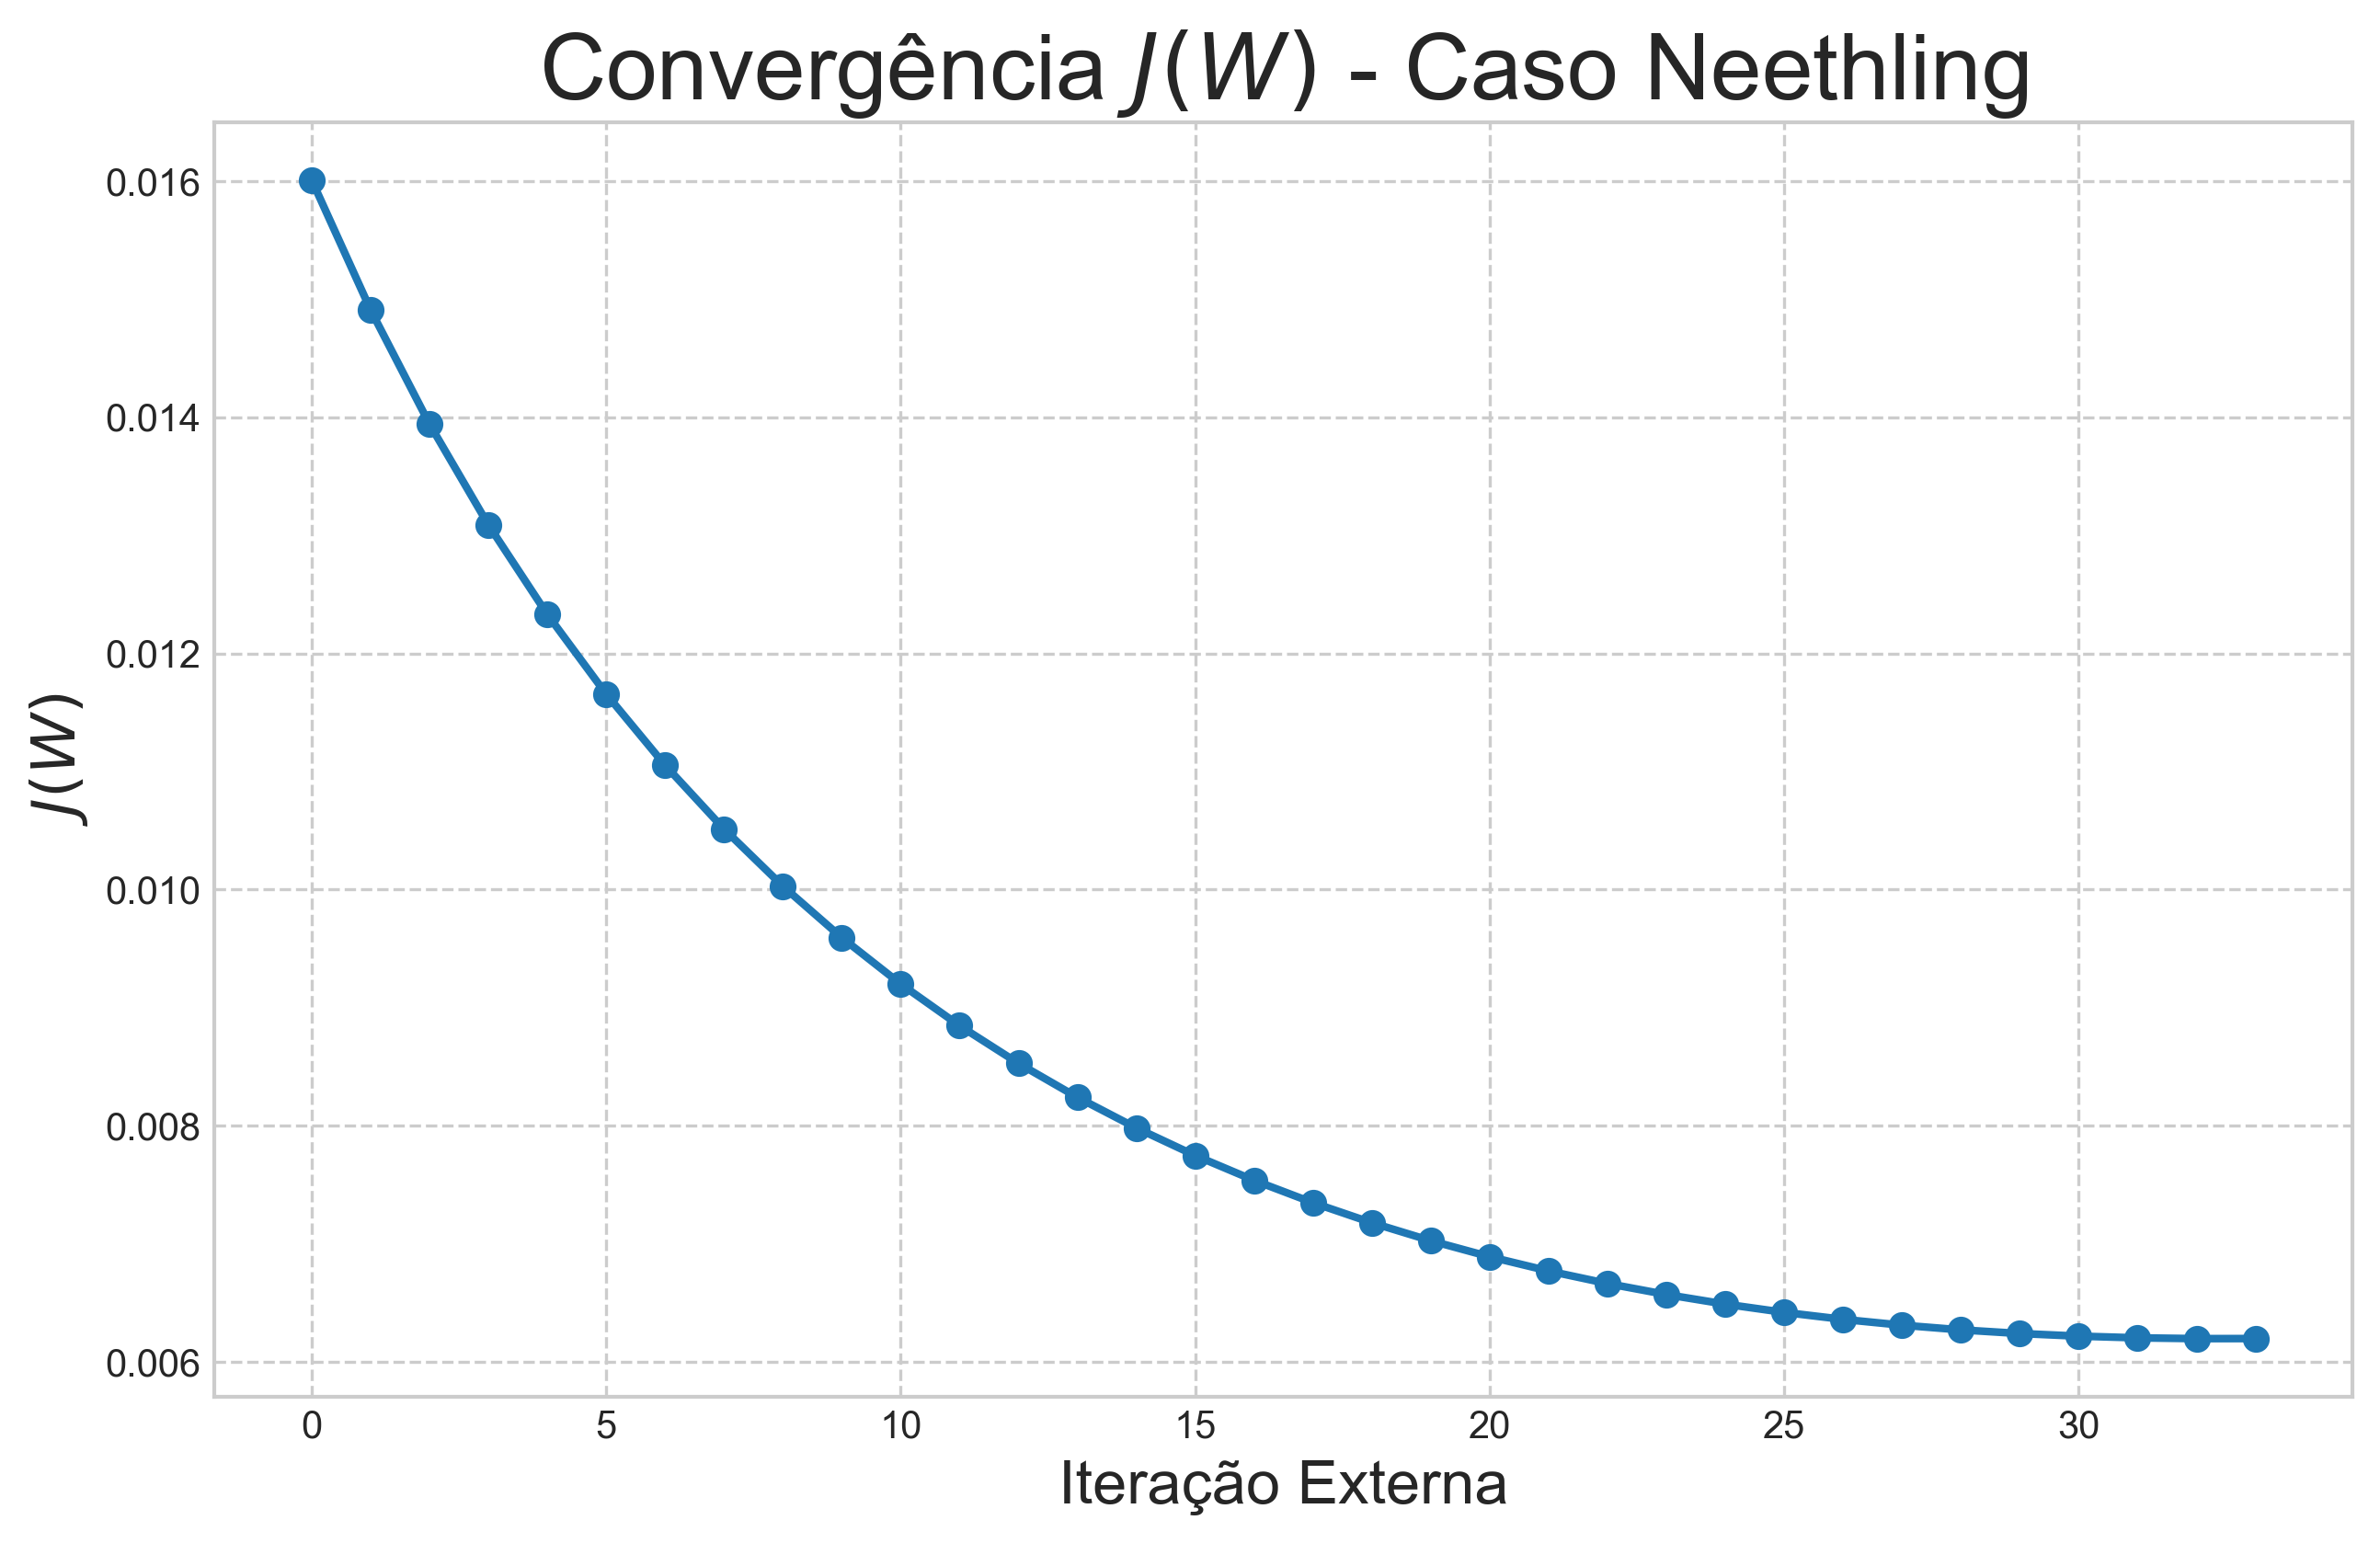
\includegraphics[width=0.85\linewidth]{Figuras/resultados/Caso_Neethling/convergencia_J_Caso_Neethling.png}
        
        \label{fig:neet_J}
        \vspace{2pt} % Pequeno ajuste de espaço
        \centerline{\footnotesize \textbf{Fonte:} Elaborado pelo autor (2026).}
\end{figure} 

\begin{figure}[H]
        \centering
        \caption{NIS resultante - Caso Neethling}
        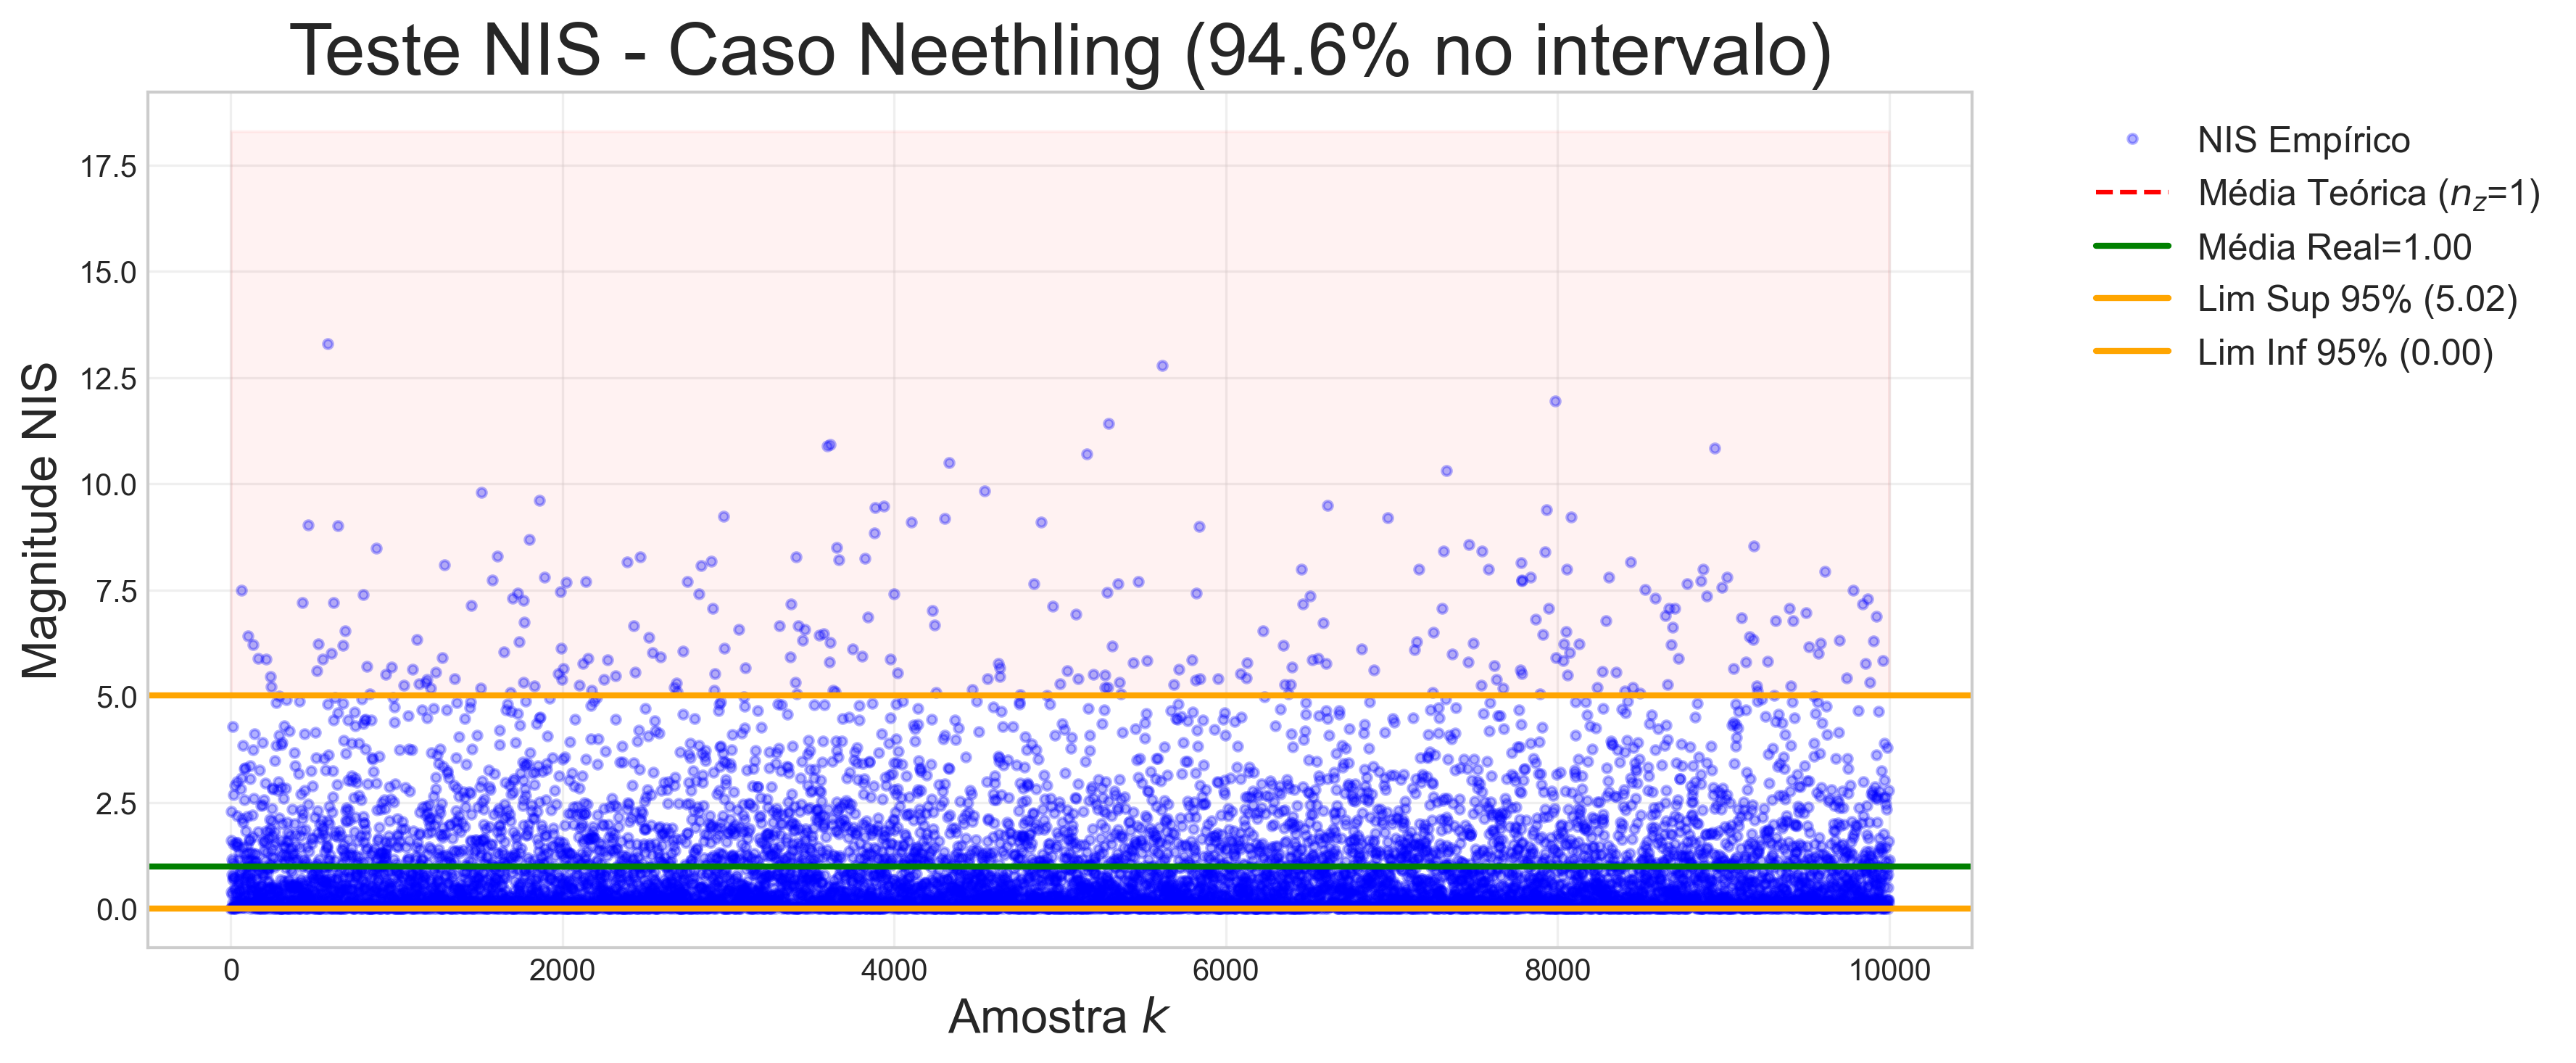
\includegraphics[width=\linewidth]{Figuras/resultados/Caso_Neethling/nis_Caso_Neethling.png}
        
        \label{fig:neet_nis}
        \vspace{2pt} % Pequeno ajuste de espaço
        \centerline{\footnotesize \textbf{Fonte:} Elaborado pelo autor (2026).}
\end{figure} 

% Teste 2
O segundo teste aplicou o modelo proposto por Odelson \cite{Odelson2006}, um conhecido caso de não identificabilidade sem a imposição de restrições estruturais. Conforme evidenciado na Tabela \ref{tab:resultado_odelson}, o posto de $\mathcal{I}$ é 8 (menor que o número de incógnitas), em contra partira ao número de variáveis livres de $\mathbf{Q}$ e $\mathbf{R}$, que são, respectivamente, 6 e 3, desrespeitando a Relação \eqref{eq:rank}, o que justifica a divergência das matrizes $\mathbf{Q}$ e $\mathbf{R}$ estimadas em relação aos valores verdadeiros.

Contudo, apesar das matrizes individuais não convergirem para os valores exatos, o algoritmo adaptativo conseguiu sintonizar o Filtro de Kalman de forma robusta. A matriz de covariância da inovação $\mathbf{S}$ alcançou os valores diagonais de $1,497$ e $0,767$, apresentando um desvio aceitável de aproximadamente $9,9\%$ e $5,6\%$, respectivamente, em relação aos elementos reais da diagonal ($1,362$ e $0,726$).

\begin{table}[H]
\centering
\caption{Resultados da Estimação Adaptativa: Caso Odelson \cite{Odelson2006}}
\label{tab:resultado_odelson}
\resizebox{\columnwidth}{!}{%
\begin{tabular}{@{}lcc@{}}
\toprule
\textbf{Parâmetro / Matriz} & \textbf{Valor Verdadeiro} & \textbf{Valor Estimado} \\ \midrule
Amostras ($N$) & \multicolumn{2}{c}{10.000} \\
Custo Mínimo $J(W)$ & --- & 0,059968 \\
Posto de $\mathcal{I}$ & \multicolumn{2}{c}{8 (Não Identificável*)} \\ \midrule
$\mathbf{Q}$ (Processo) & 
$\begin{bmatrix} 0.1 & 0 & 0 \\ 0 & 0.2 & 0 \\ 0 & 0 & 0.1 \end{bmatrix}$ & 
$\begin{bmatrix} 0.207 & 0.400 & 0.005 \\ 0.400 & 0.776 & -0.015 \\ 0.005 & -0.015 & 0.320 \end{bmatrix}$ \\ \addlinespace

$\mathbf{R}$ (Medição) & 
$\begin{bmatrix} 0.5 & 0 \\ 0 & 0.5 \end{bmatrix}$ & 
$\begin{bmatrix} 0.286 & 0.007 \\ 0.007 & 0.301 \end{bmatrix}$ \\ \addlinespace

$\mathbf{W}$ (Ganho) & 
$\begin{bmatrix} 0.207 & 0.000 \\ 0.633 & 0.000 \\ 0.000 & 0.311 \end{bmatrix}$ & 
$\begin{bmatrix} 0.363 & 0.005 \\ 0.805 & -0.007 \\ 0.000 & 0.603 \end{bmatrix}$ \\ \addlinespace

$\mathbf{S}$ (Inovação) & 
$\begin{bmatrix} 1.362 & 0.000 \\ 0.000 & 0.726 \end{bmatrix}$ & 
$\begin{bmatrix} 1.497 & -0.002 \\ -0.002 & 0.767 \end{bmatrix}$ \\ \bottomrule
\multicolumn{3}{l}{\scriptsize *Identificável apenas se for imposta estrutura diagonal a $\mathbf{Q}$.}
\end{tabular}%
}
\vspace{1pt}
    \centerline{\footnotesize \textbf{Fonte:} Elaborado pelo autor (2026).}
\end{table}

O decaimento da métrica $J(\mathbf{W})$ e a convergência do algoritmo para este caso adverso podem ser analisados na Figura \ref{fig:odel_J}. O gráfico do NIS (Figura \ref{fig:odel_nis}) é particularmente importante neste caso: mesmo sem recuperar os verdadeiros $\mathbf{Q}$ e $\mathbf{R}$, a média empírica do NIS se estabeleceu próxima do esperado ($n_z=2$), provando que a "mentira" paramétrica gerou uma sintonia operacionalmente funcional e conservadora, além de se manter no intervalo esperado.

\begin{figure}[H]
        \centering
        \caption{Função Erro $J(\mathbf{W})$ - Caso Odelson}
        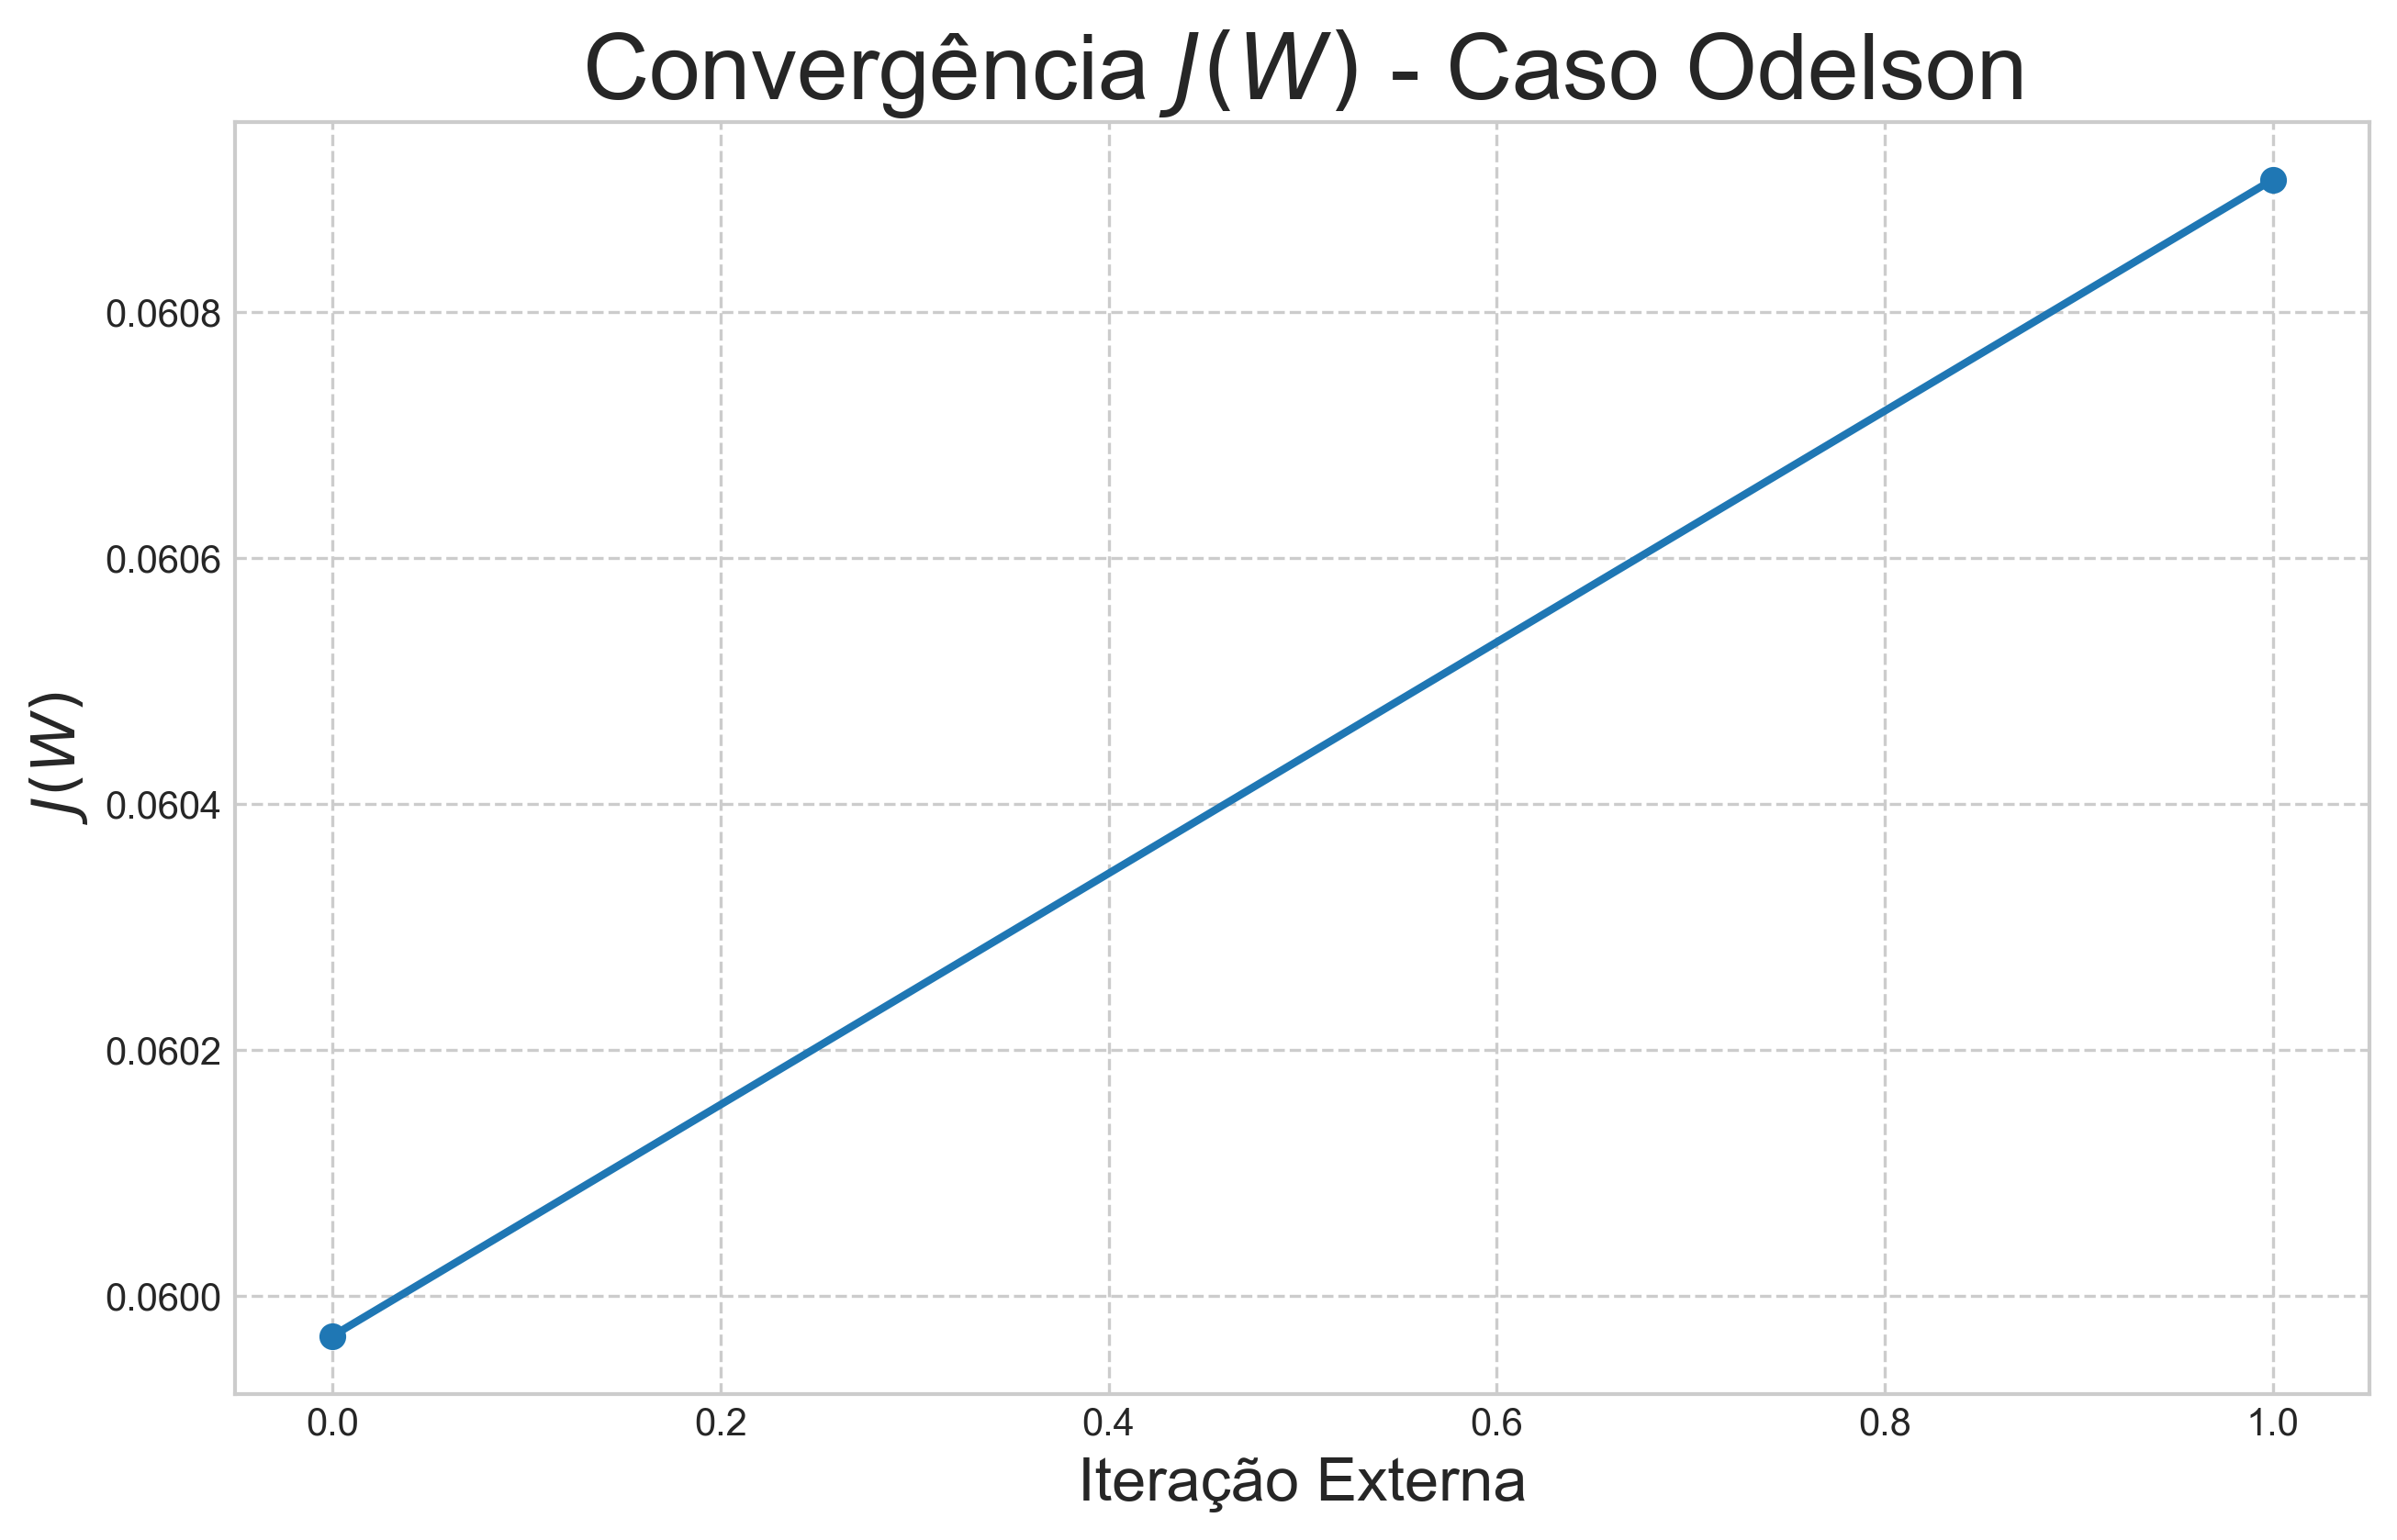
\includegraphics[width=0.85\linewidth]{Figuras/resultados/Caso_Odelson/convergencia_J_Caso_Odelson.png}
        
        \label{fig:odel_J}
        \vspace{2pt} % Pequeno ajuste de espaço
        \centerline{\footnotesize \textbf{Fonte:} Elaborado pelo autor (2026).}
\end{figure} 

\begin{figure}[H]
        \centering
        \caption{NIS resultante - Caso Neethling}
        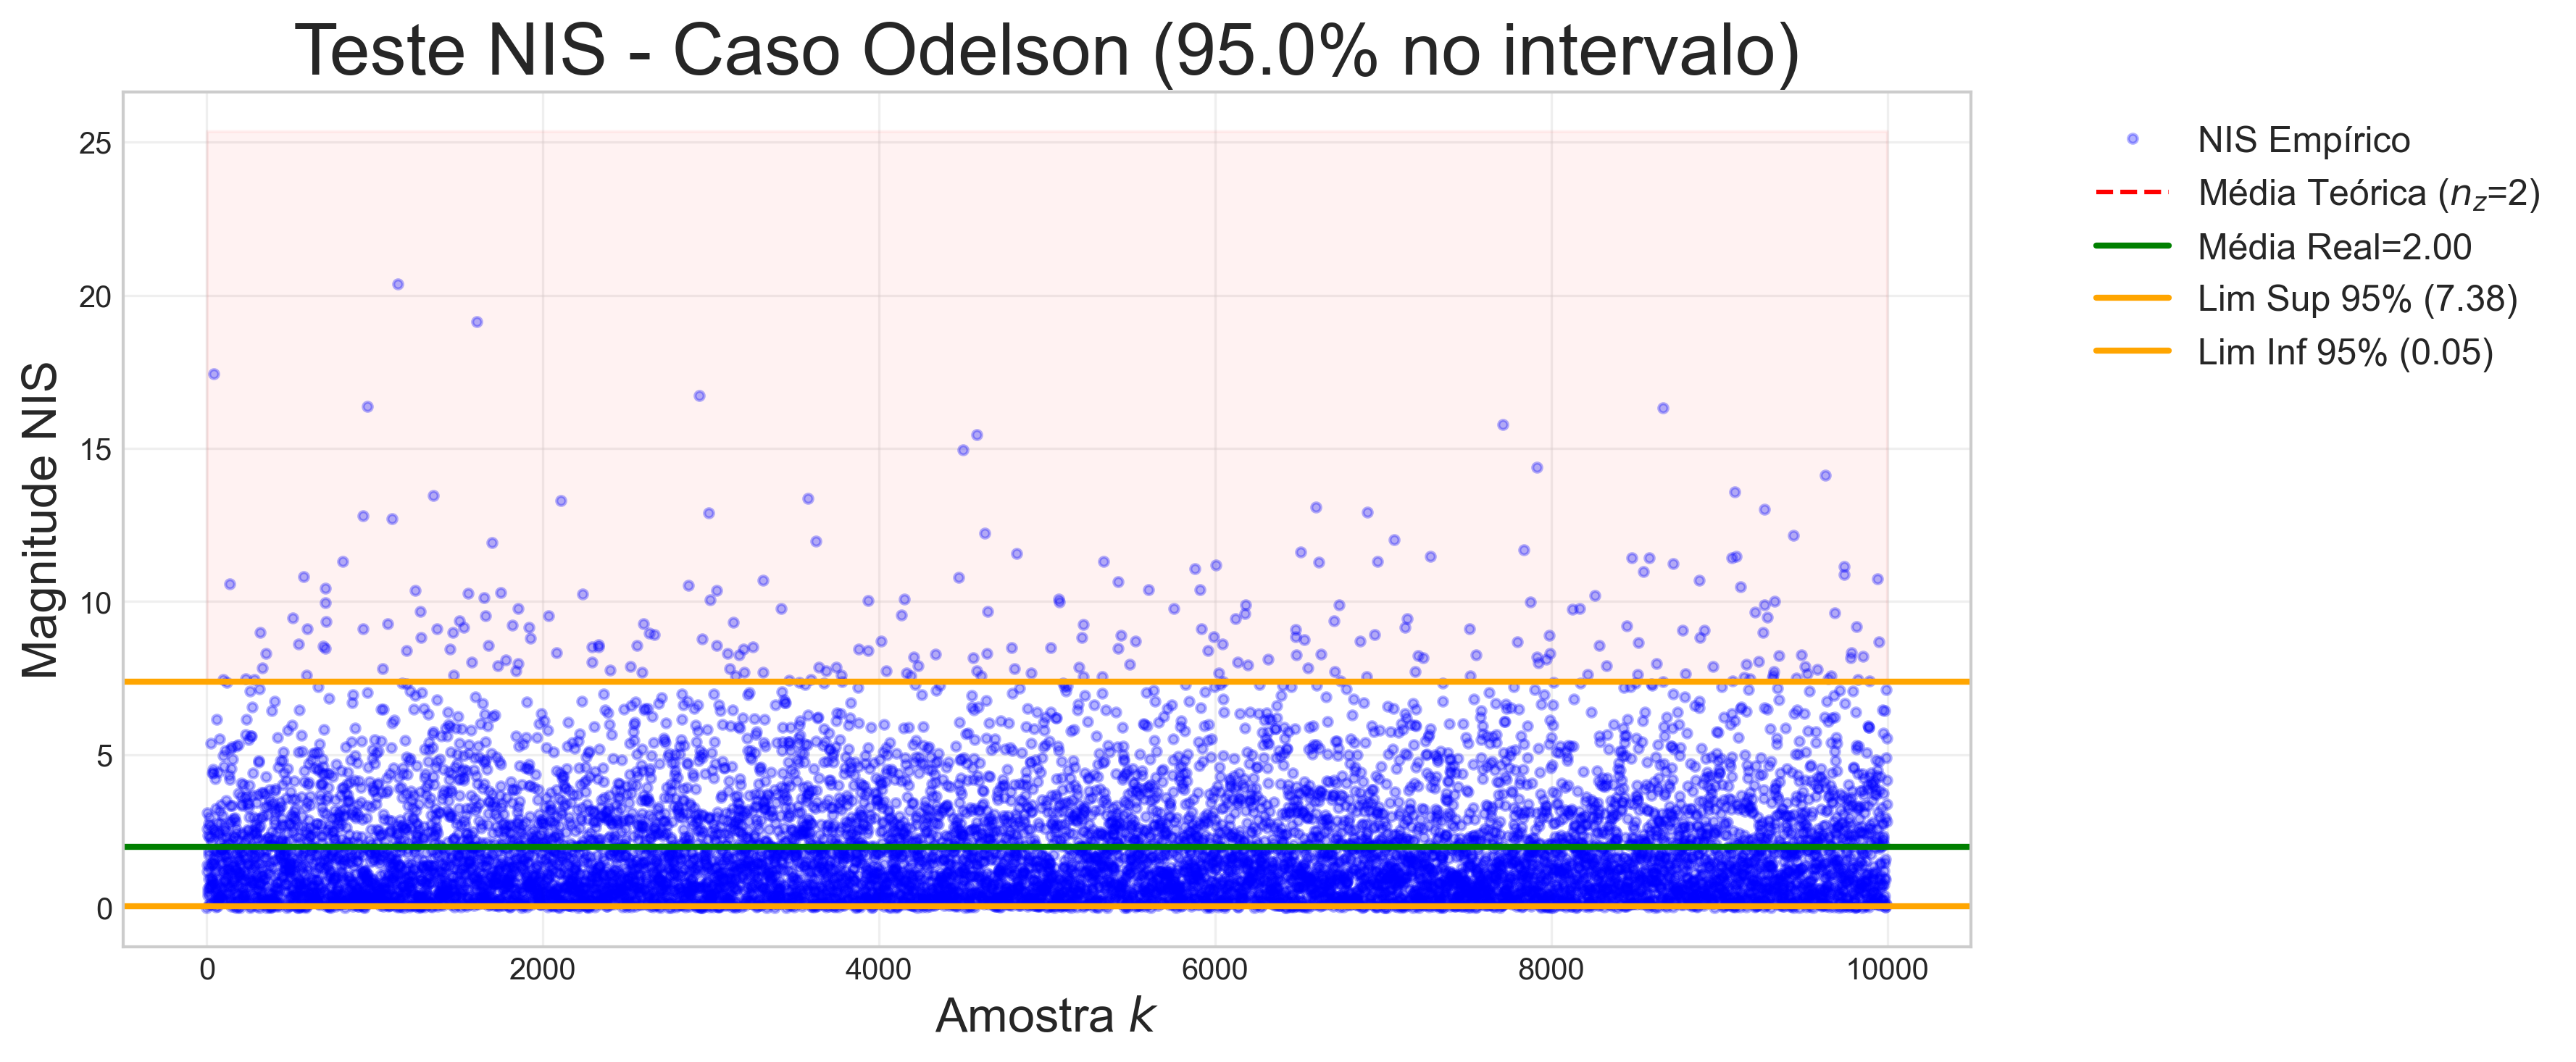
\includegraphics[width=\linewidth]{Figuras/resultados/Caso_Odelson/nis_Caso_Odelson.png}
        
        \label{fig:odel_nis}
        \vspace{2pt} % Pequeno ajuste de espaço
        \centerline{\footnotesize \textbf{Fonte:} Elaborado pelo autor (2026).}
\end{figure} 


% Teste 3 
Por fim, o Caso de Mehra \cite{Mehra1970} foi simulado utilizando uma base ampla de $100.000$ amostras, em um sistema plenamente identificável de alta ordem (Posto de $\mathcal{I}$ = 9), pois o número de incógnitas livres de $Q$ é 6 e o número de incógnitas livres de $R$ é 3, portanto, respeita a Relação \ref{eq:rank}. A Tabela \ref{tab:resultado_Mehra} evidencia os melhores resultados relativos dentre os cenários testados. 

A matriz $\mathbf{R}$ estimada retornou diagonais de $0,584$ e $0,474$, apresentando um erro de desvio inferior a $17\%$ e $5,2\%$, respectivamente, comparado ao referencial de $0,500$. Mais impressionante é a estimativa da inovação $\mathbf{S}$: o elemento principal $S_{11}$ real foi de $7,978$, enquanto o estimado cravou $8,033$ (uma fidelidade superior a $99,3\%$).

\begin{table}[H]
\centering
\caption{Resultados da Estimação Adaptativa: Caso Mehra \cite{Mehra1970}}
\label{tab:resultado_Mehra}
\resizebox{\columnwidth}{!}{% % Garante que a tabela caiba na largura da coluna
\begin{tabular}{@{}lcc@{}}
\toprule
\textbf{Parâmetro / Matriz} & \textbf{Valor Verdadeiro} & \textbf{Valor Estimado} \\ \midrule
Amostras ($N$) & \multicolumn{2}{c}{100.000} \\
Custo Mínimo $J(W)$ & --- & 0,011406 \\
Posto de $\mathcal{I}$ & \multicolumn{2}{c}{9 (Identificável)} \\ \midrule
$\mathbf{Q}$ (Processo) & 
$\begin{bmatrix} 0.1 & 0 & 0 \\ 0 & 0.2 & 0 \\ 0 & 0 & 0.1 \end{bmatrix}$ & 
$\begin{bmatrix} 0.127 & -0.027 & 0.023 \\ -0.027 & 0.188 & -0.231 \\ 0.023 & -0.231 & 0.284 \end{bmatrix}$ \\ \addlinespace

$\mathbf{R}$ (Medição) & 
$\begin{bmatrix} 0.5 & 0 \\ 0 & 0.5 \end{bmatrix}$ & 
$\begin{bmatrix} 0.584 & 0.169 \\ 0.169 & 0.474 \end{bmatrix}$ \\ \addlinespace

$\mathbf{W}$ (Ganho) & 
$\begin{bmatrix} 0.906 & 0.362 \\ 0.004 & 0.214 \\ -2.564 & -0.951 \\ 0.000 & 0.177 \\ 0.030 & -0.357 \end{bmatrix}$ & 
$\begin{bmatrix} 0.905 & 0.728 \\ -0.007 & 0.237 \\ -2.854 & -1.510 \\ -0.005 & 0.223 \\ 0.020 & -0.886 \end{bmatrix}$ \\ \addlinespace

$\mathbf{S}$ (Inovação) & 
$\begin{bmatrix} 7.978 & 0.062 \\ 0.062 & 0.822 \end{bmatrix}$ & 
$\begin{bmatrix} 8.033 & 0.048 \\ 0.048 & 0.848 \end{bmatrix}$ \\ \bottomrule
\end{tabular}%
}
\vspace{1pt}
    \centerline{\footnotesize \textbf{Fonte:} Elaborado pelo autor (2026).}
\end{table}

Esses resultados robustos são suportados pelas Figuras \ref{fig:mehra_J} e \ref{fig:mehra_nis}. A convergência da minimização de $J(\mathbf{W})$ foi bem-sucedida atingindo o patamar de $0,0114$, acompanhada de uma distribuição de erros estabilizada e validada pelo limite de confiança do NIS.

\begin{figure}[H]
        \centering
        \caption{Função Erro $J(\mathbf{W})$ - Caso Mehra}
        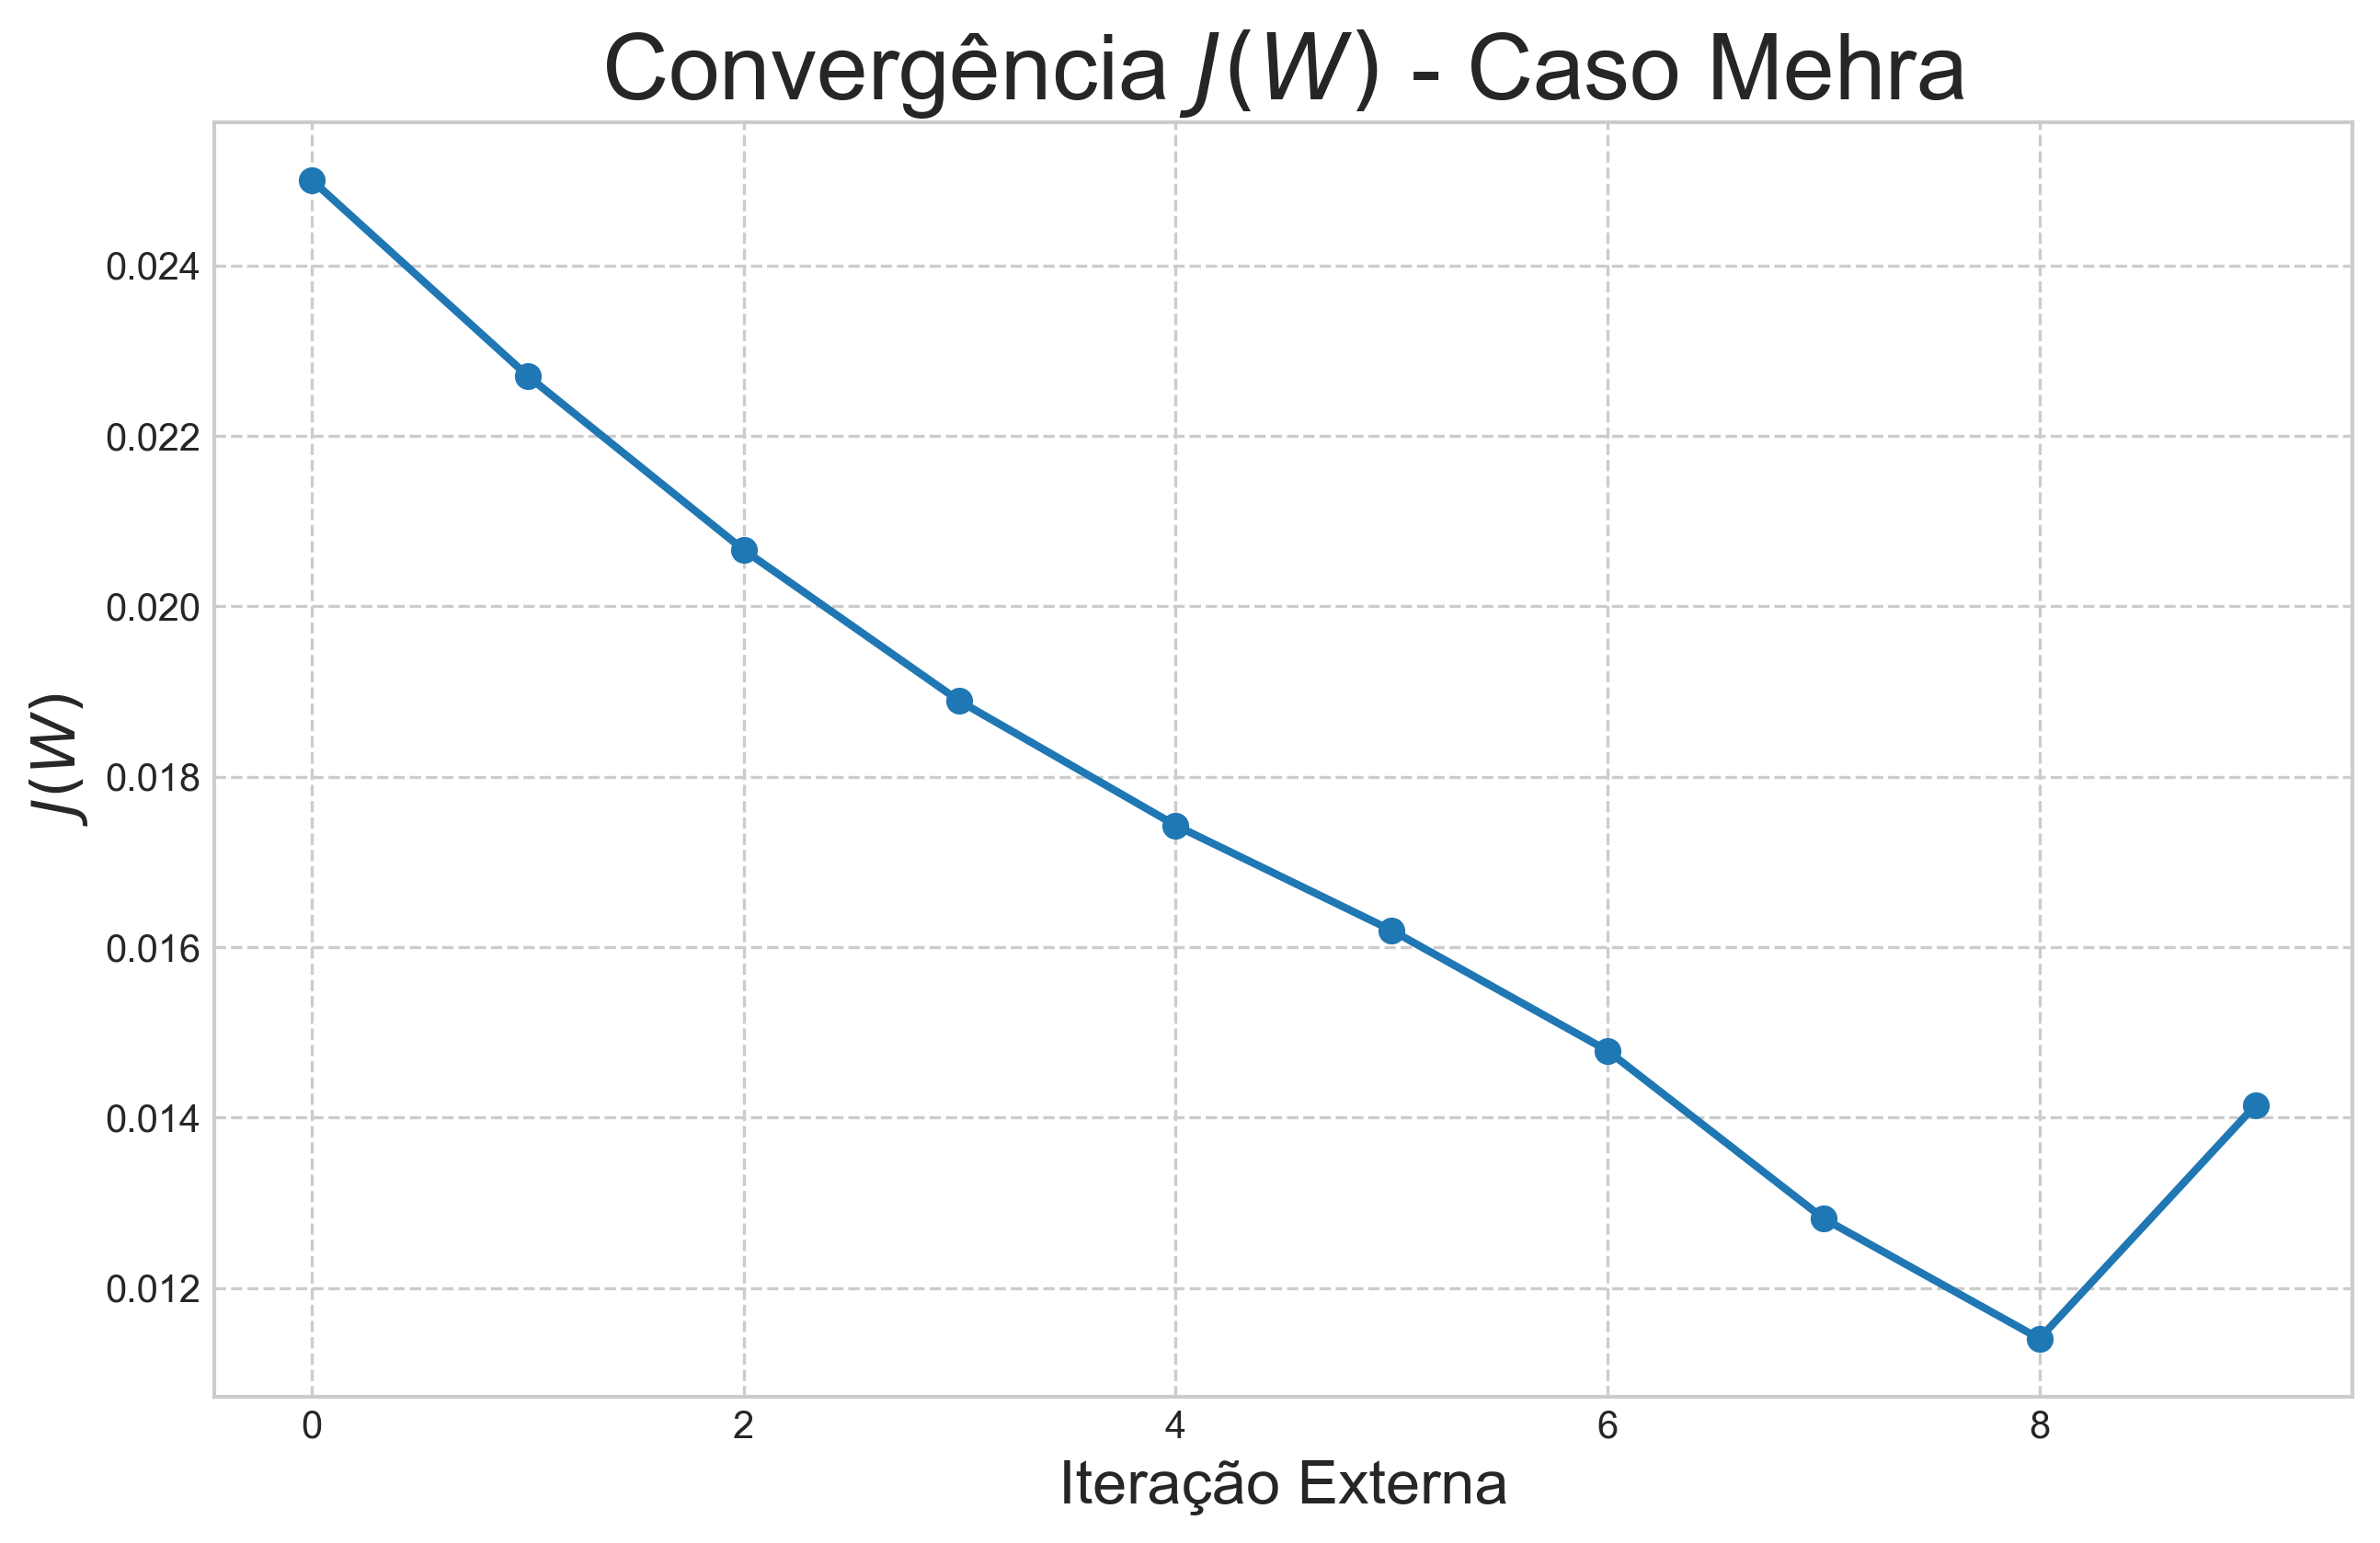
\includegraphics[width=0.85\linewidth]{Figuras/resultados/Caso_Mehra/convergencia_J_Caso_Mehra.png}
        
        \label{fig:mehra_J}
        \vspace{2pt} % Pequeno ajuste de espaço
        \centerline{\footnotesize \textbf{Fonte:} Elaborado pelo autor (2026).}
\end{figure} 

\begin{figure}[H]
        \centering
        \caption{NIS resultante - Caso Mehra}
        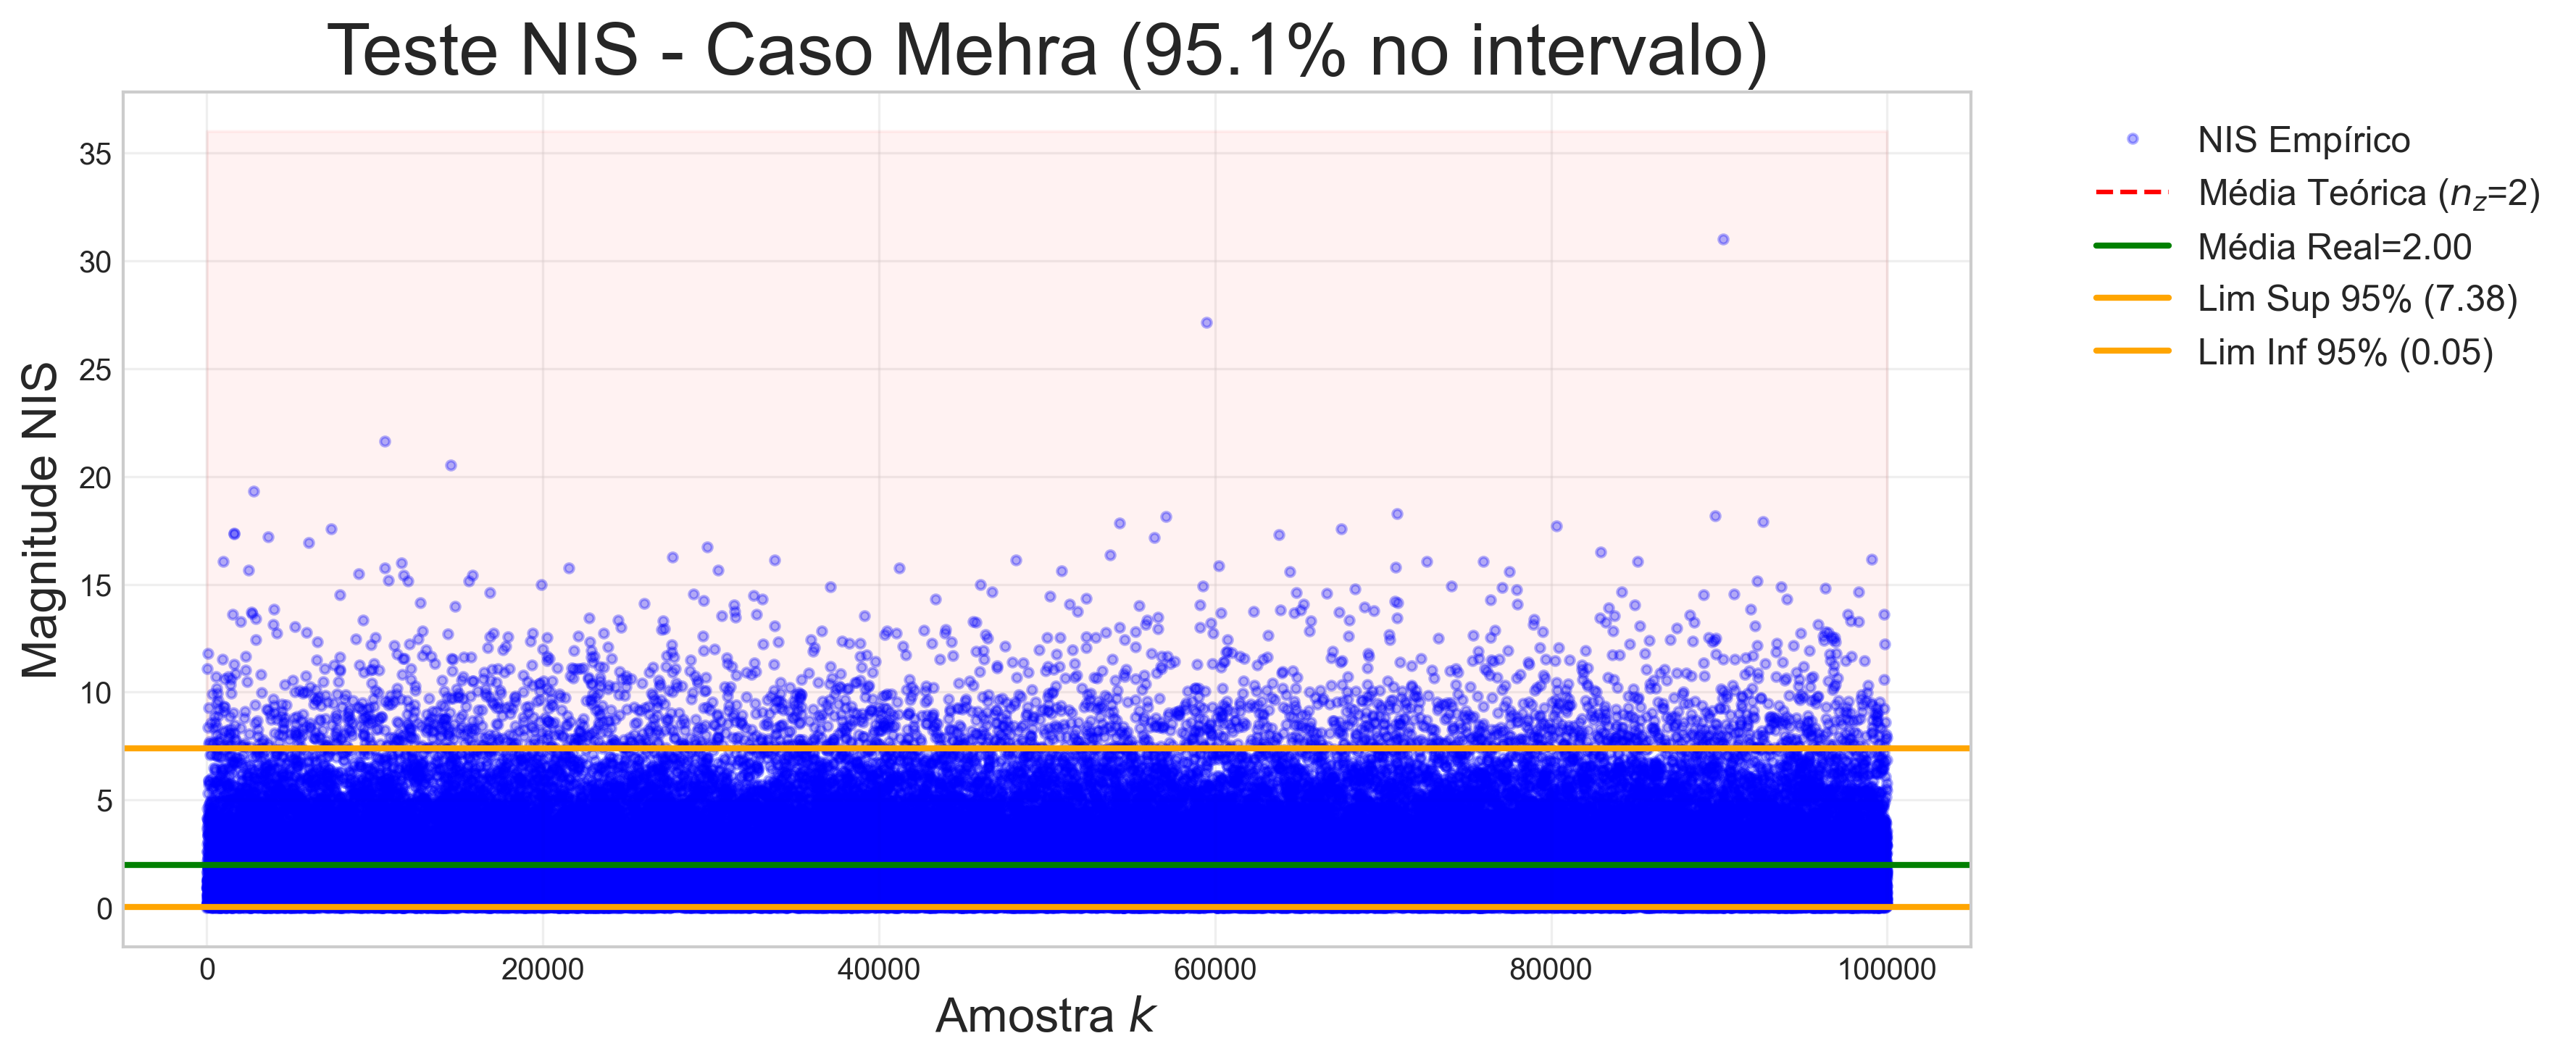
\includegraphics[width=\linewidth]{Figuras/resultados/Caso_Mehra/nis_Caso_Mehra.png}
        
        \label{fig:mehra_nis}
        \vspace{2pt} % Pequeno ajuste de espaço
        \centerline{\footnotesize \textbf{Fonte:} Elaborado pelo autor (2026).}
\end{figure} 


\subsection{Trajetória 1}

A trajetória quadrada representa um cenário de estresse para estimadores cinemáticos, pois impõe mudanças abruptas de direção que se traduzem em degraus de velocidade. Conforme ilustrado na Figura \ref{fig:EkfQuadrado}, o Filtro de Kalman Estendido (EKF) apresentou uma capacidade de rastreamento robusta, mantendo a estabilidade mesmo nos pontos de descontinuidade da derivada da trajetória.

A avaliação quantitativa do erro de estado, apresentada na Figura \ref{fig:ErrosQuadrado}, indica que os picos de erro ocorrem predominantemente nas quinas do quadrado, onde a aceleração sofre variações instantâneas não modeladas perfeitamente pelo regime PVA. Observa-se, contudo, que após o transiente de manobra, os erros residuais retornam rapidamente à zona de confiança estatística. Os erros de velocidade situam-se no intervalo de $\pm 2$ m/s, enquanto os erros de posição mantêm-se em um intervalo de 95\% de confiança entre -1,25 m e 1,25 m. 

Este desempenho é considerado satisfatório dado que, para lados de 600 metros, o erro RMS de 0,7173 m (Tabela \ref{tab:resultados_estatisticos2}) representa um erro percentual relativo de aproximadamente \textbf{0,12\%}. Contudo, deve-se notar que a utilização dos valores fixos da Tabela \ref{tab:param_ekf_traj} pode induzir a uma superestimação do filtro em cenários reais menos controlados devido às covariâncias reduzidas.

% EKF Gerado
\begin{figure}[H]
        \centering
        \caption{Trajetória - Quadrado - EKF}
        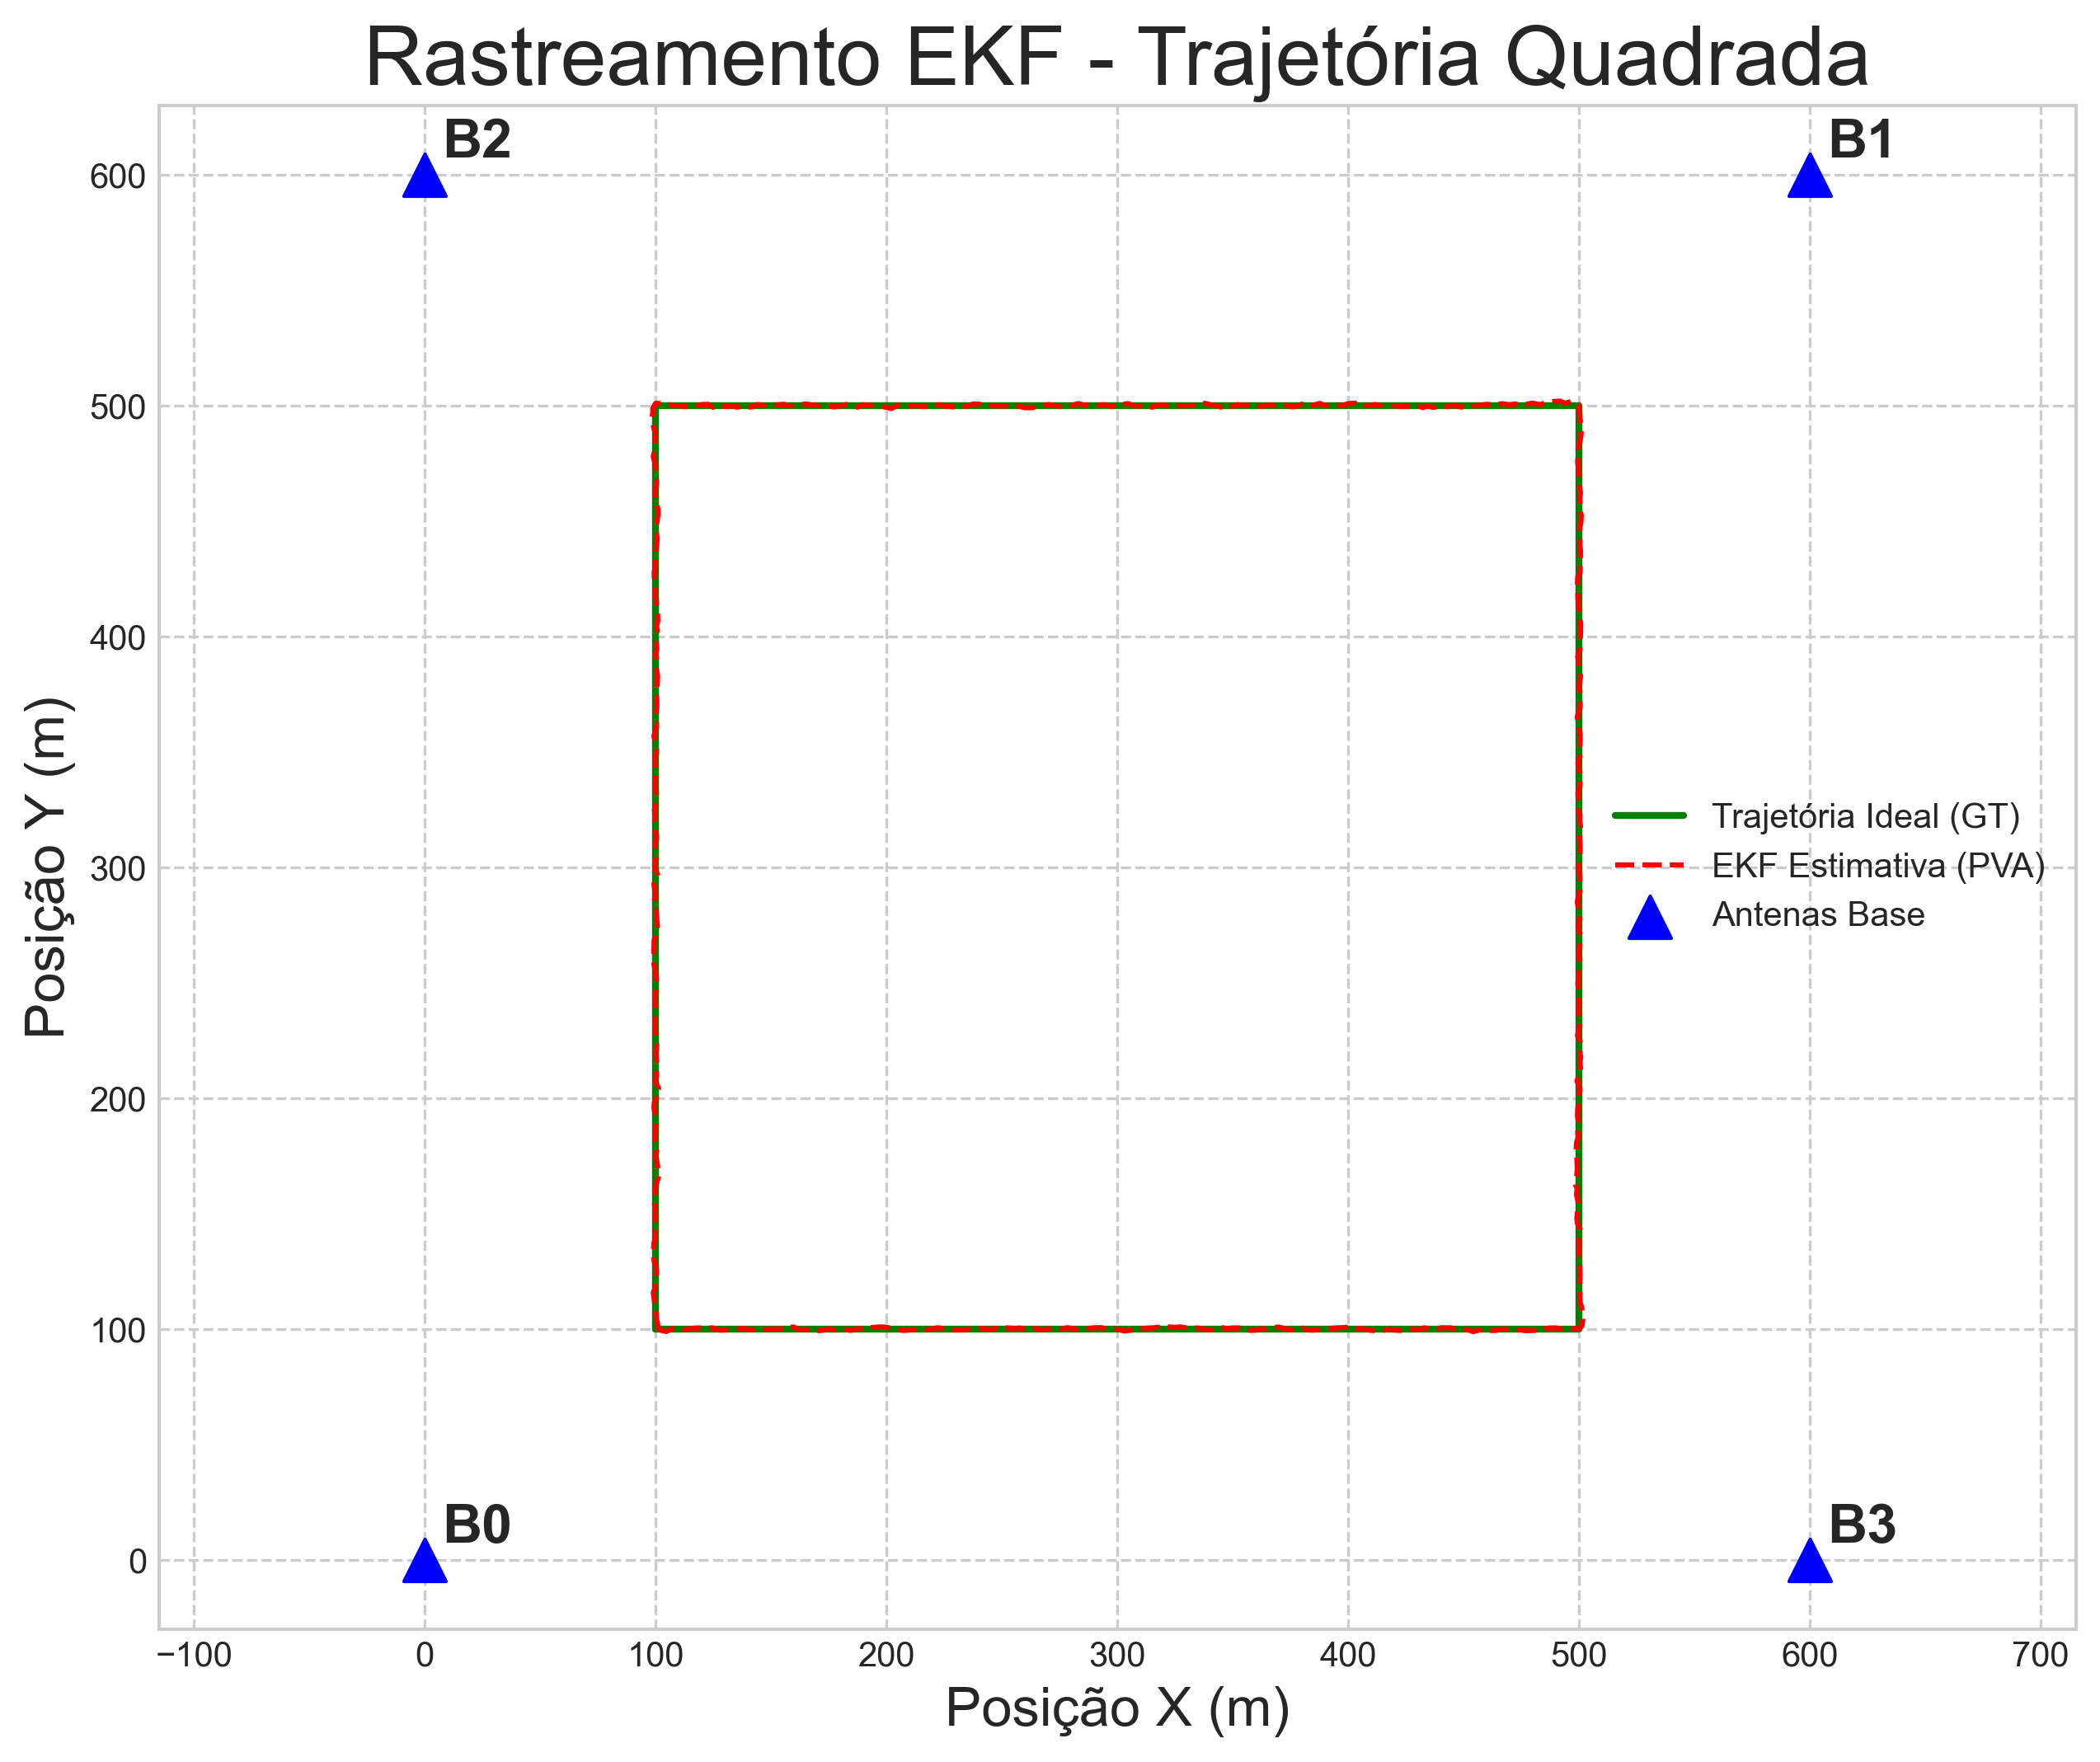
\includegraphics[width=0.85\linewidth]{Figuras/resultados/trajetoria_pva_quadrada/trajetoria_pva_quadrada.png}
        
        \label{fig:EkfQuadrado}
        \vspace{2pt} % Pequeno ajuste de espaço
        \centerline{\footnotesize \textbf{Fonte:} Elaborado pelo autor (2026).}
\end{figure} 

% Gráficos de Erros 
\begin{figure}[H]
        \centering
        \caption{Trajetória - Quadrado - Erros }
        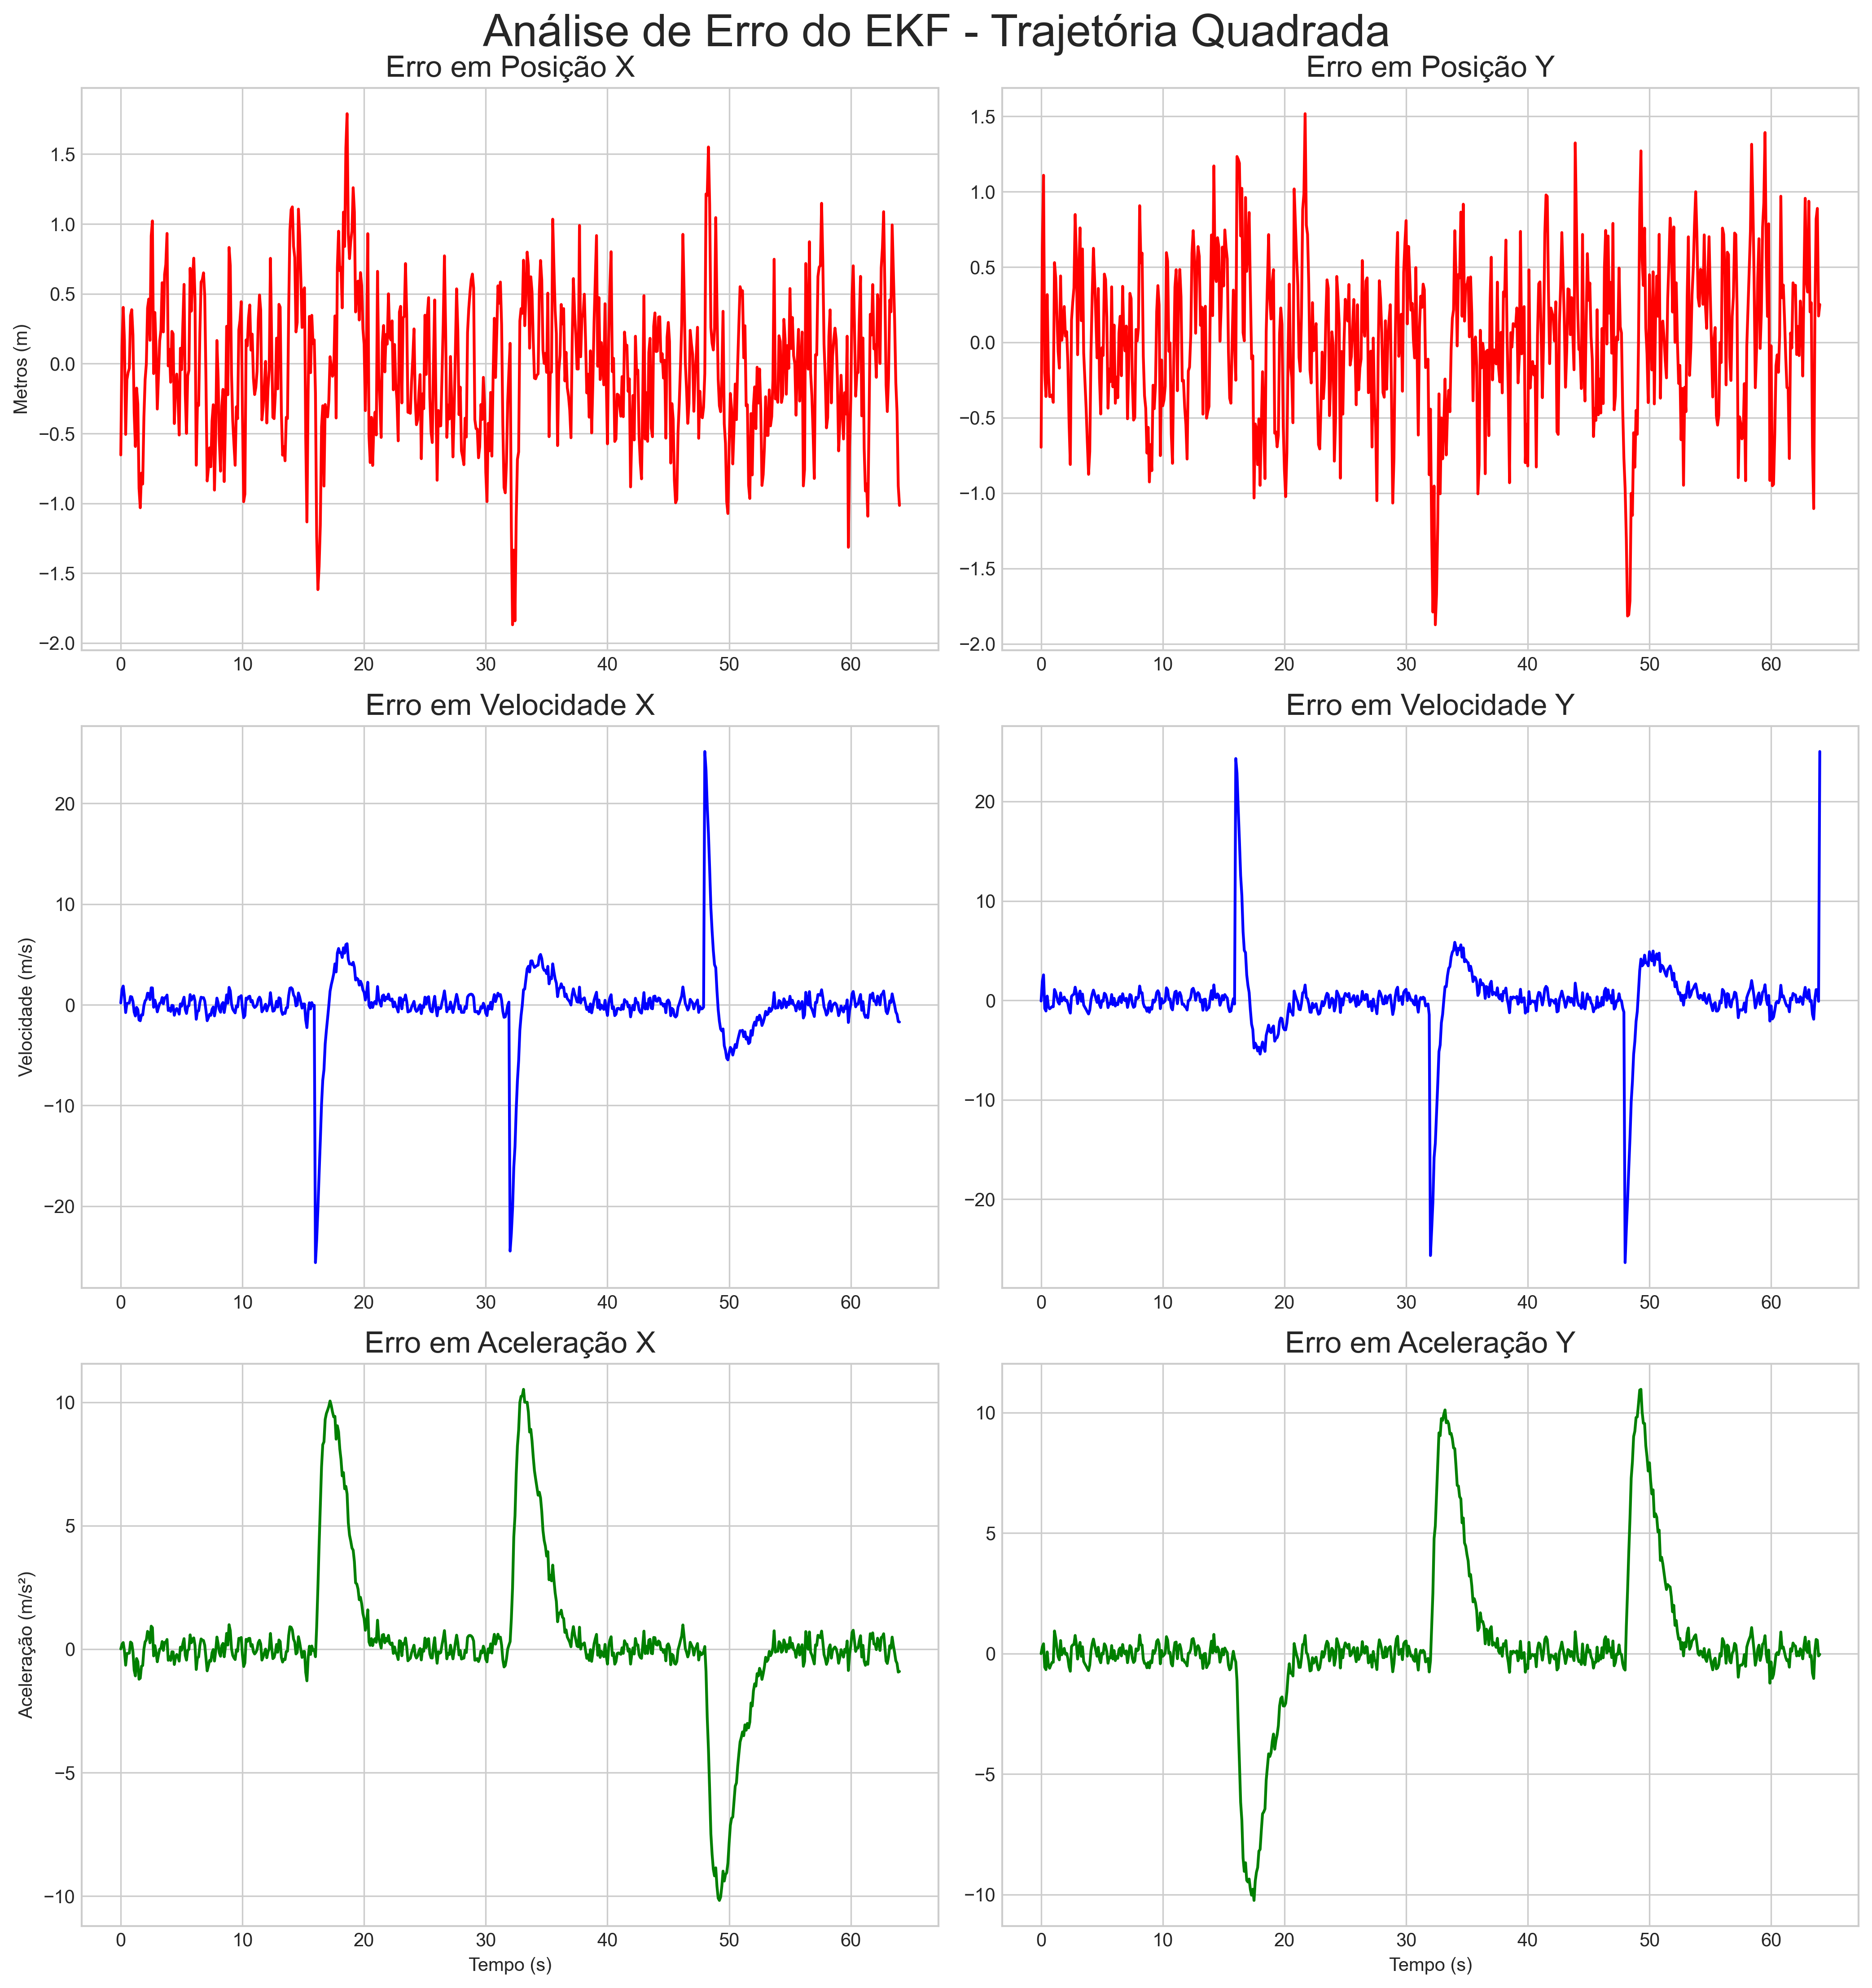
\includegraphics[width=0.85\linewidth]{Figuras/resultados/trajetoria_pva_quadrada/erros_estados_pva_quadrada.png}
        
        \label{fig:ErrosQuadrado}
        \vspace{2pt} % Pequeno ajuste de espaço
        \centerline{\footnotesize \textbf{Fonte:} Elaborado pelo autor (2026).}
\end{figure} 


% Tabelas 
\subsection{Trajetória 2}

O cenário circular impõe uma dinâmica de aceleração centrípeta constante, desafiando a capacidade do estimador em lidar com vetores de estado permanentemente variantes. A Figura \ref{fig:EksCircular} demonstra que a trajetória estimada apresenta uma sobreposição precisa à trajetória real, sugerindo que a parametrização adotada permitiu um ajuste de ganho adequado para este regime dinâmico.

Os gráficos de erro na Figura \ref{fig:ErrosCircular} exibem um comportamento oscilatório amortecido, típico de rastreamento de alvos em curvas de raio constante. A estabilidade dos erros em regime permanente corrobora a eficácia do algoritmo. Para este cenário, os erros de posição oscilaram entre $\pm 1,5$ m e os de velocidade entre $\pm 2,5$ m/s, com uma variância de velocidade calculada em \textbf{5,41 m²/s²} (derivada do DP de 2,3275 m/s da Tabela \ref{tab:resultados_estatisticos2}). Assim como na trajetória anterior, os dados consolidados na Tabela \ref{tab:resultados_estatisticos2} confirmam a precisão do rastreamento sob aceleração constante.


% EKF Gerado
\begin{figure}[H]
\centering
\caption{Trajetória - Circular - EKF}
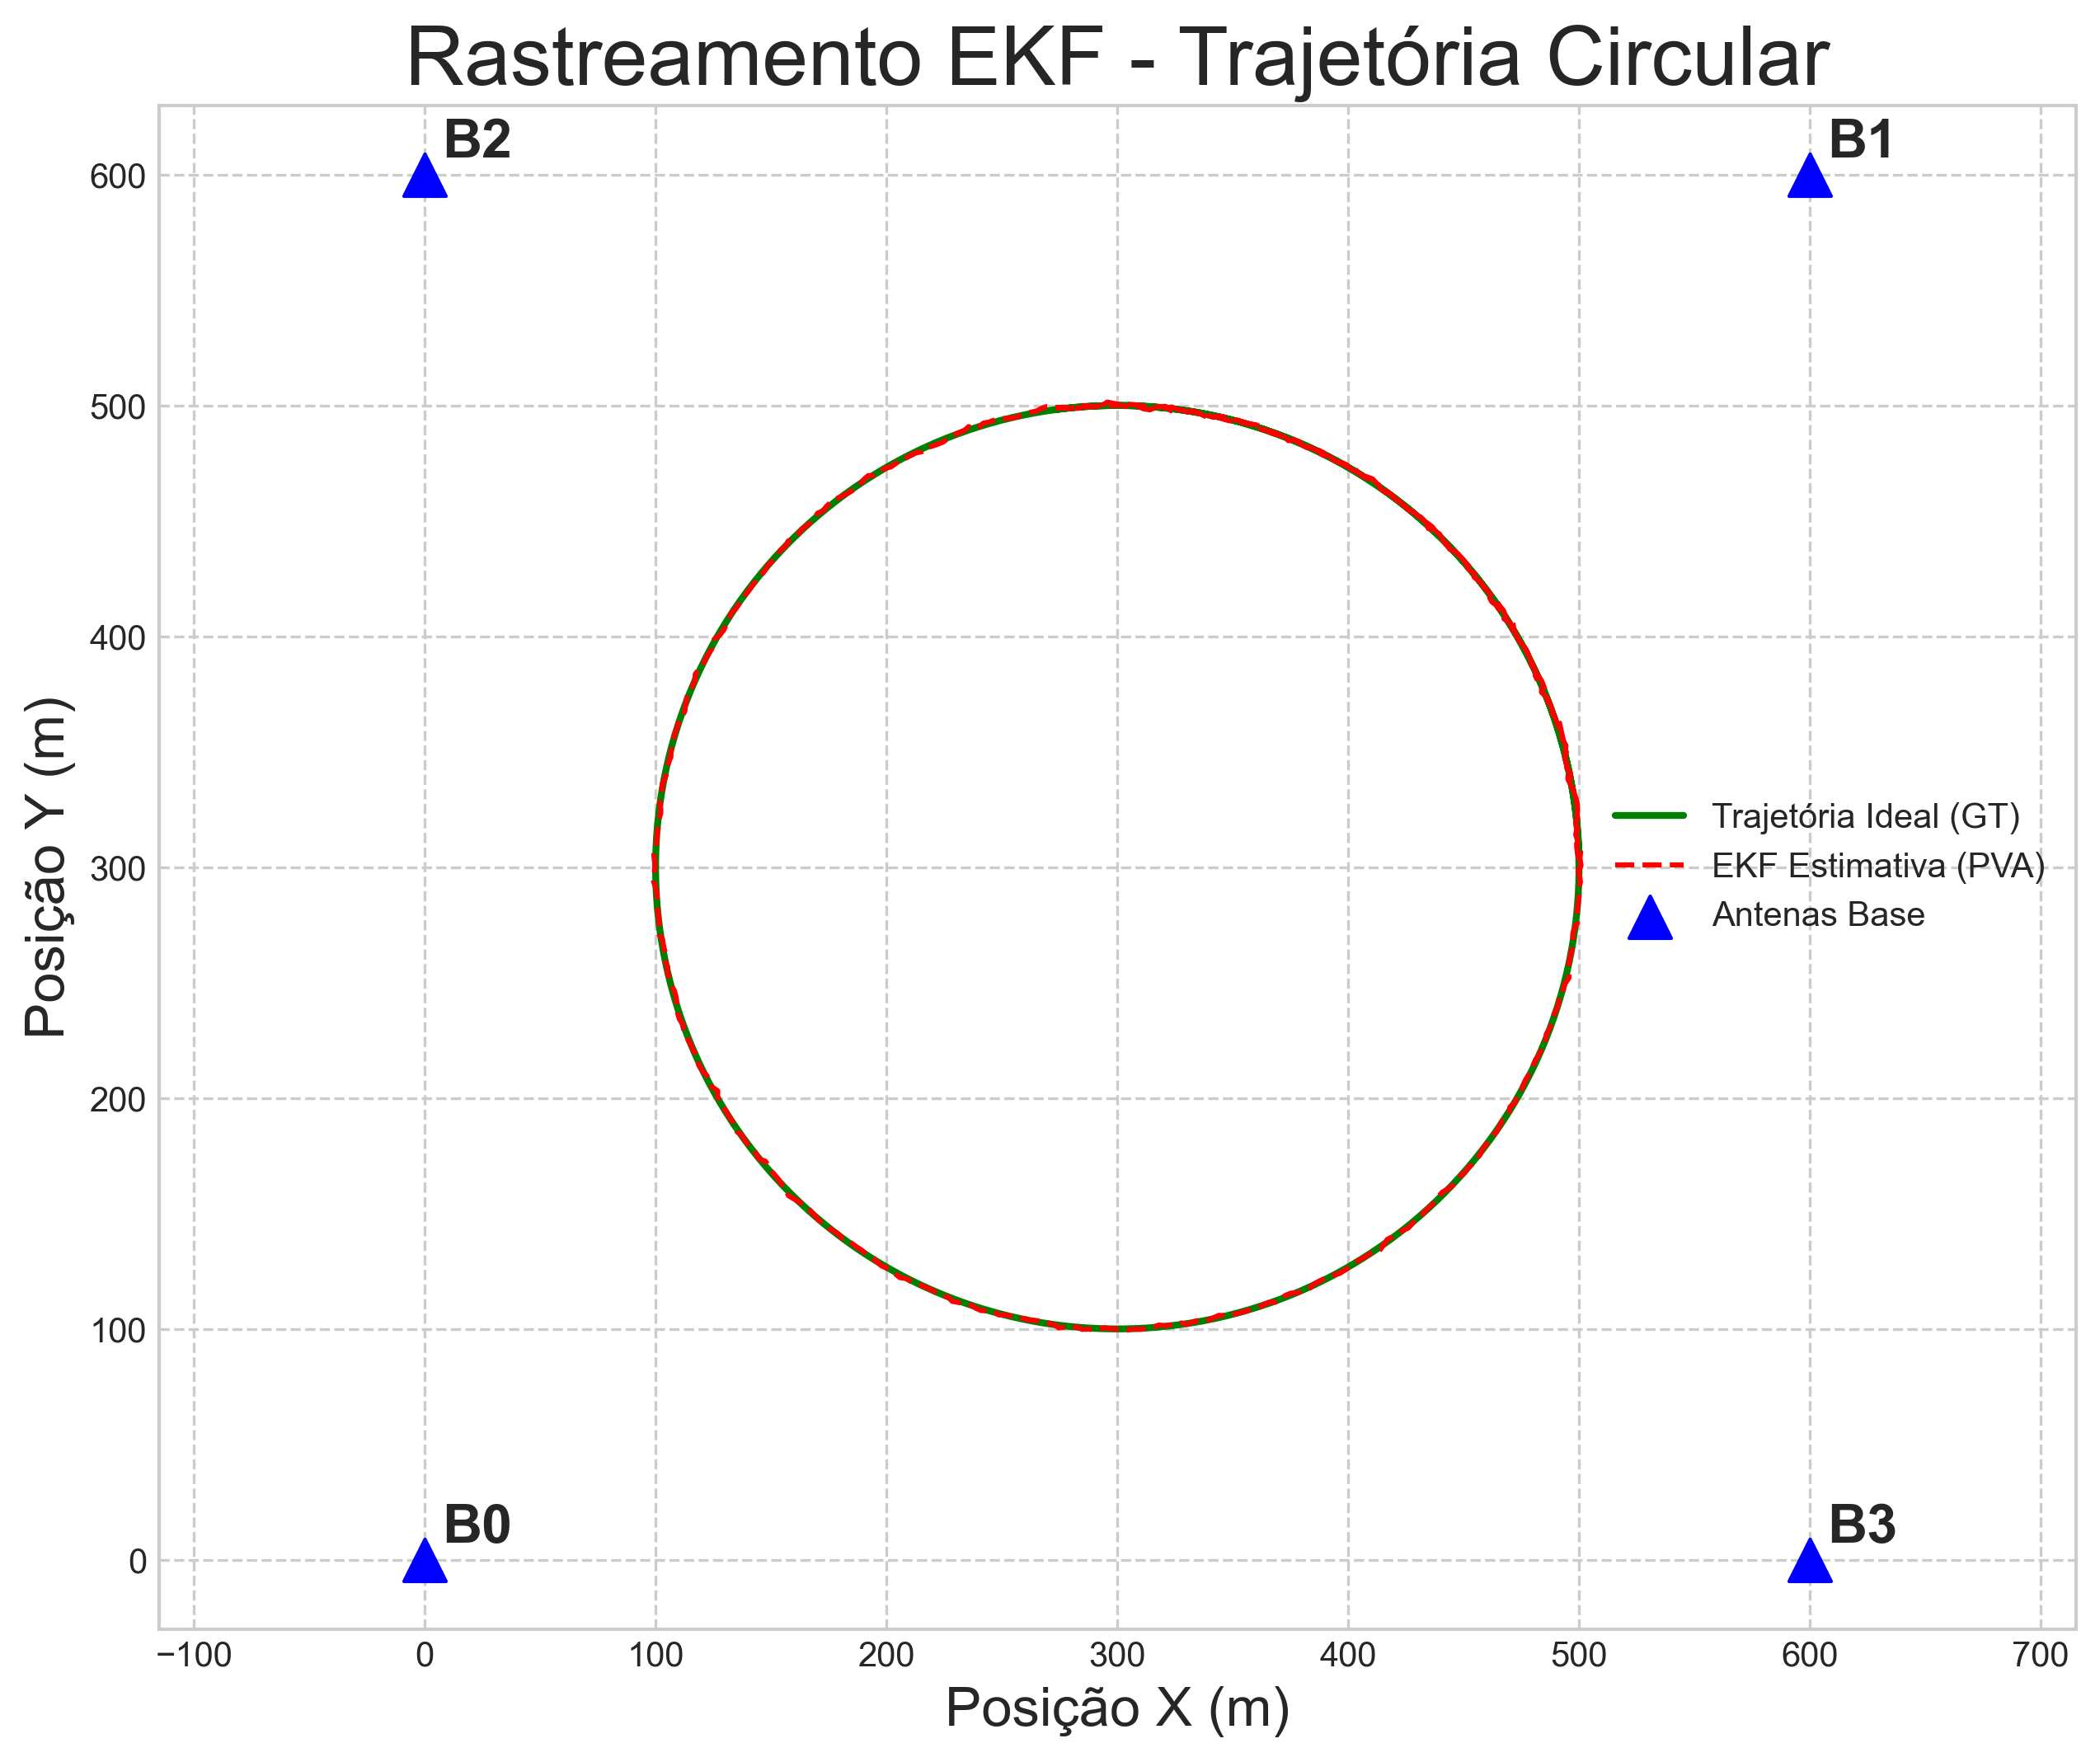
\includegraphics[width=0.85\linewidth]{Figuras/resultados/trajetoria_pva_circular/trajetoria_pva_circular.png}
\label{fig:EksCircular}
\vspace{2pt} % Pequeno ajuste de espaço
        \centerline{\footnotesize \textbf{Fonte:} Elaborado pelo autor (2026).}
\end{figure} 

% Gráficos de Erros 
\begin{figure}[H]
        \centering
        \caption{Trajetória - Circular - Erros }
        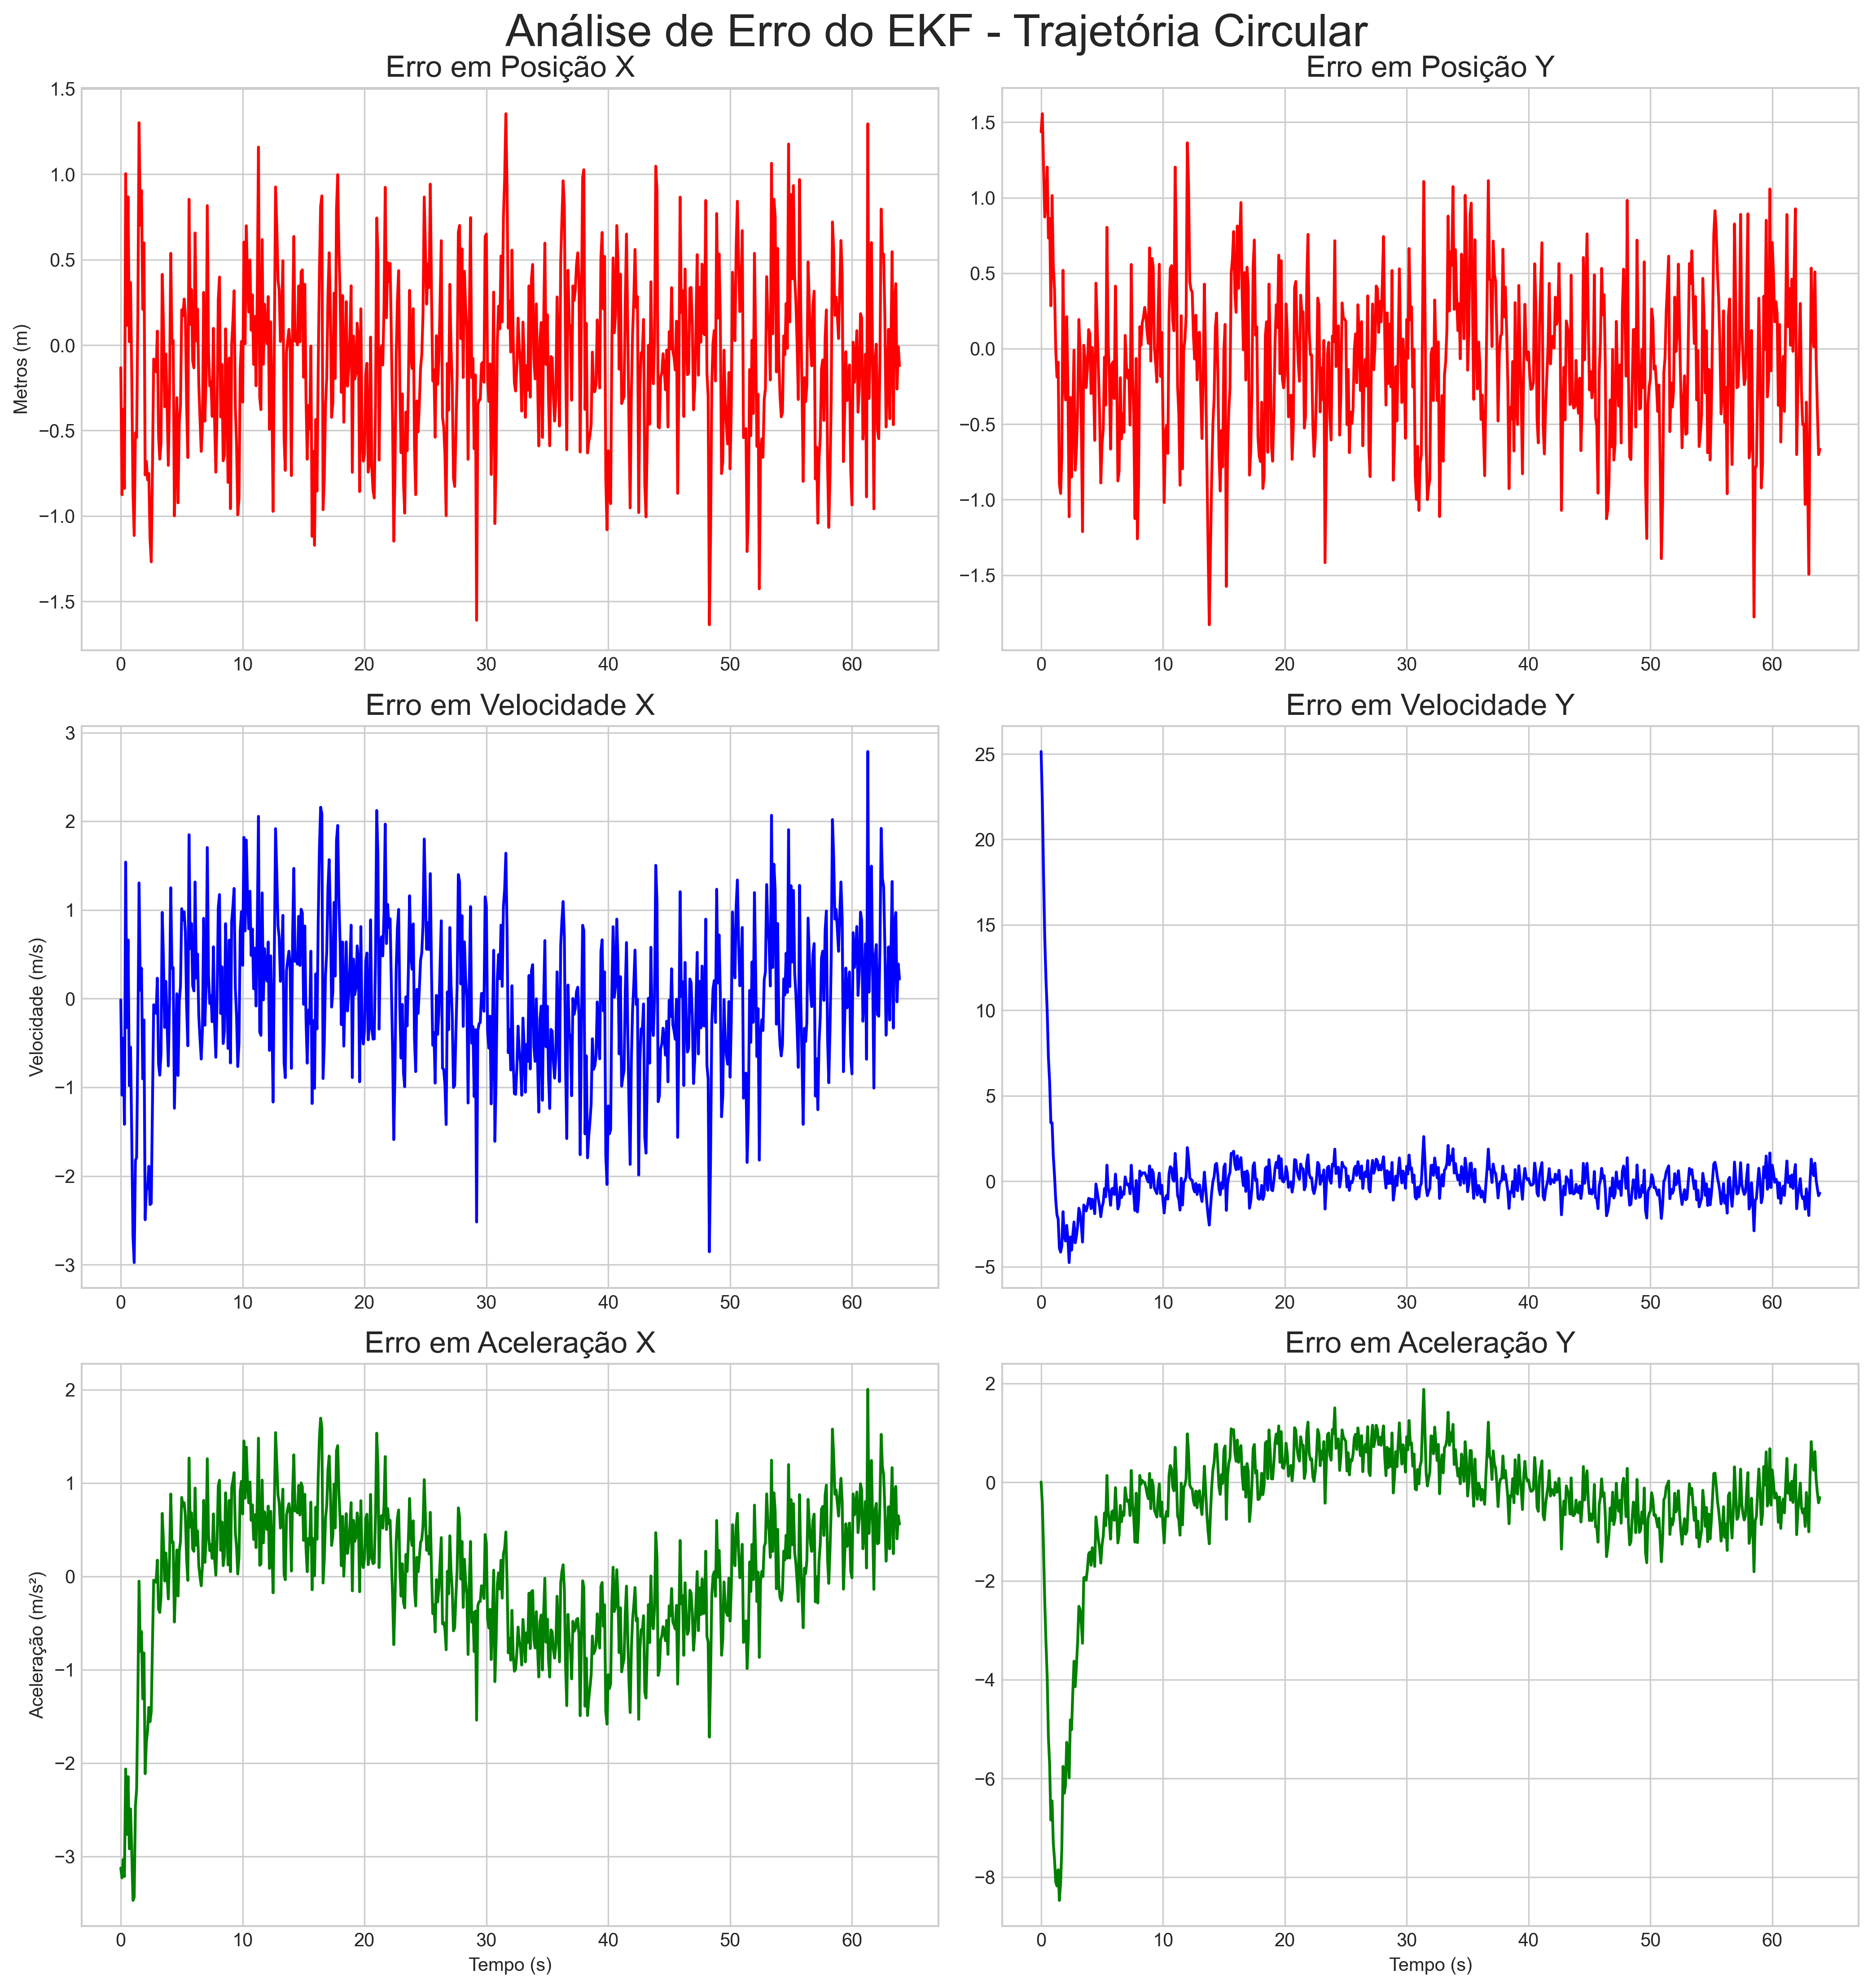
\includegraphics[width=0.85\linewidth]{Figuras/resultados/trajetoria_pva_circular/erros_estados_pva_circular.png}
        \label{fig:ErrosCircular}
        \vspace{2pt} % Pequeno ajuste de espaço
        \centerline{\footnotesize \textbf{Fonte:} Elaborado pelo autor (2026).}
\end{figure} 

% Tabelas 
\subsection{Trajetória 3}

A trajetória baseada na função tangente hiperbólica (Figura \ref{fig:EksCurvaS_Traj}) representa o cenário de maior complexidade dinâmica devido à variação contínua da curvatura. Este perfil exige que o filtro acompanhe transições suaves, porém rápidas, entre trechos retilíneos e curvos de diferentes raios.

A análise dos erros de estado na Figura \ref{fig:ErrosCurvaS} revela que o filtro mantém um desempenho superior aos cenários anteriores, apresentando um RMS de posição de apenas 0,6553 m. Embora ocorra uma elevação marginal no erro durante os pontos de inflexão da curva, o sistema demonstra rápida recuperação. Os erros de velocidade permaneceram contidos no intervalo de $\sigma 1,5$ m/s, evidenciando que, para dinâmicas mais suaves, o modelo PVA integrado aos parâmetros da Tabela \ref{tab:param_ekf_traj} atinge alta eficiência.

% EKF Gerado
\begin{figure}[H]
        \centering
        \caption{Trajetória - Curva S - EKF}
        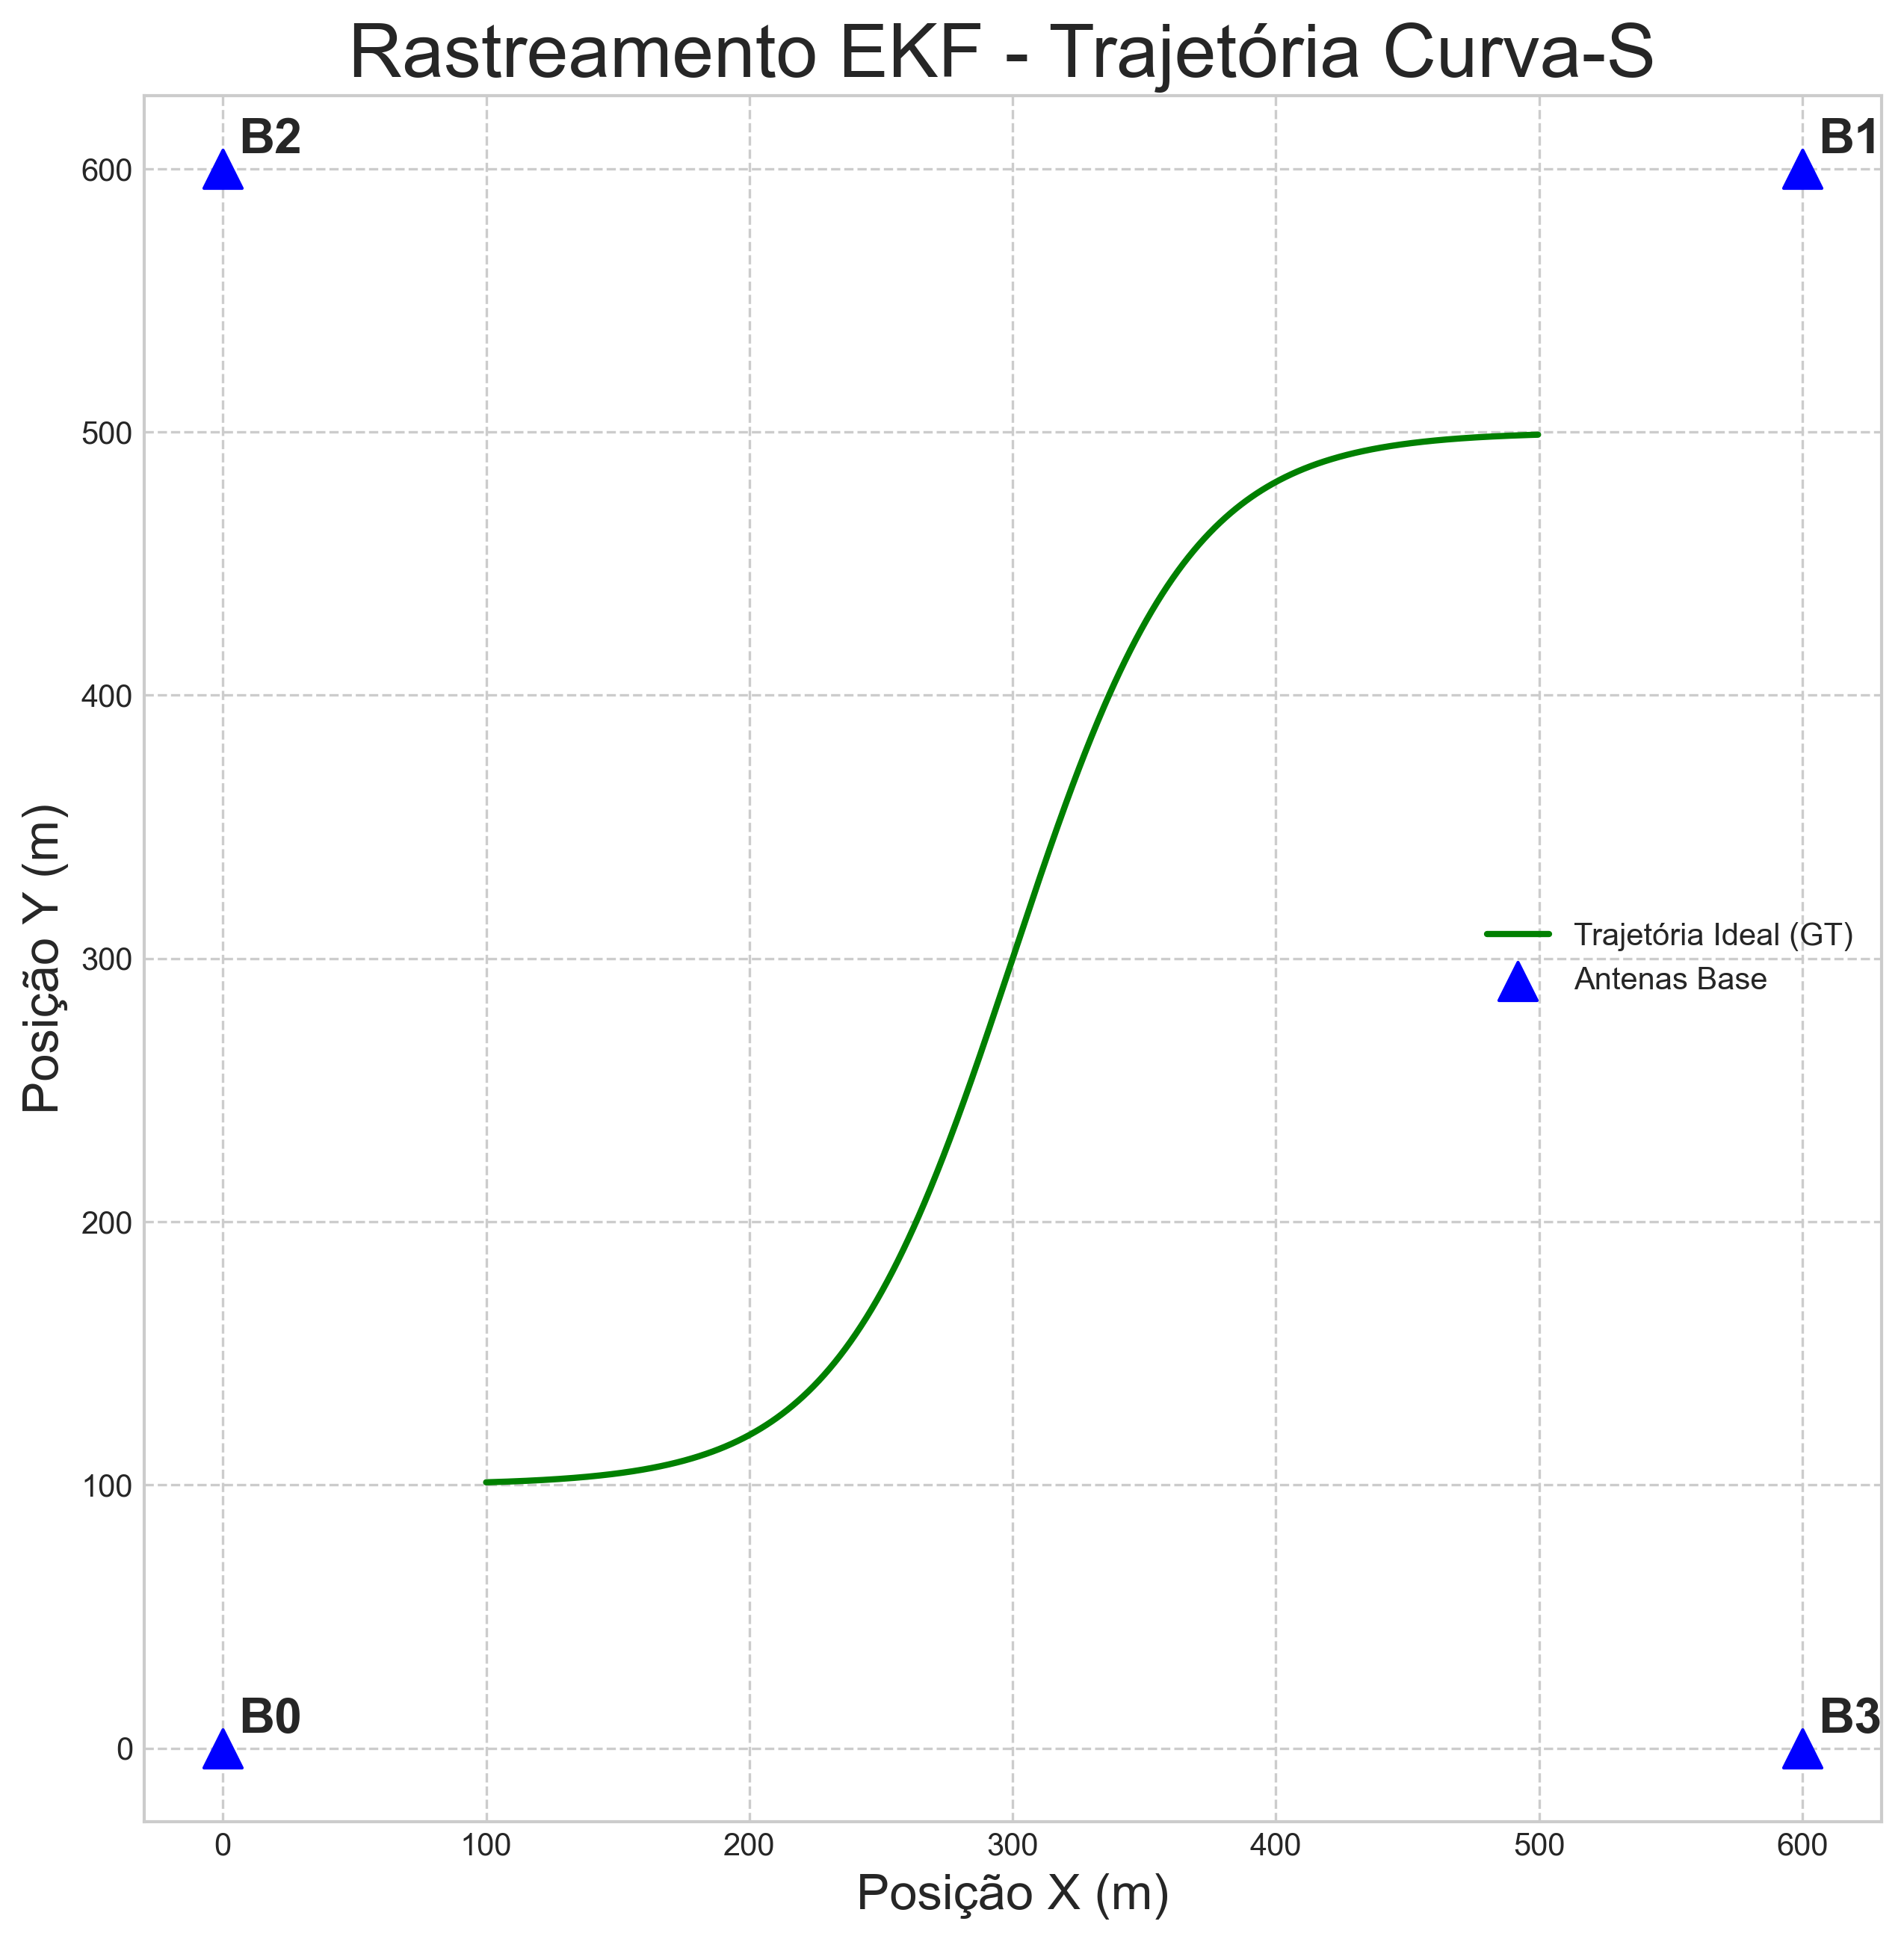
\includegraphics[width=0.85\linewidth]{Figuras/resultados/trajetoria_pva_curva_s/trajetoria_curva_s.png}
        \label{fig:EksCurvaS}
        \vspace{2pt} % Pequeno ajuste de espaço
        \centerline{\footnotesize \textbf{Fonte:} Elaborado pelo autor (2026).}
\end{figure} 

% Gráficos de Erros 
\begin{figure}[H]
        \centering
        \caption{Trajetória - Curva S - Erros }
        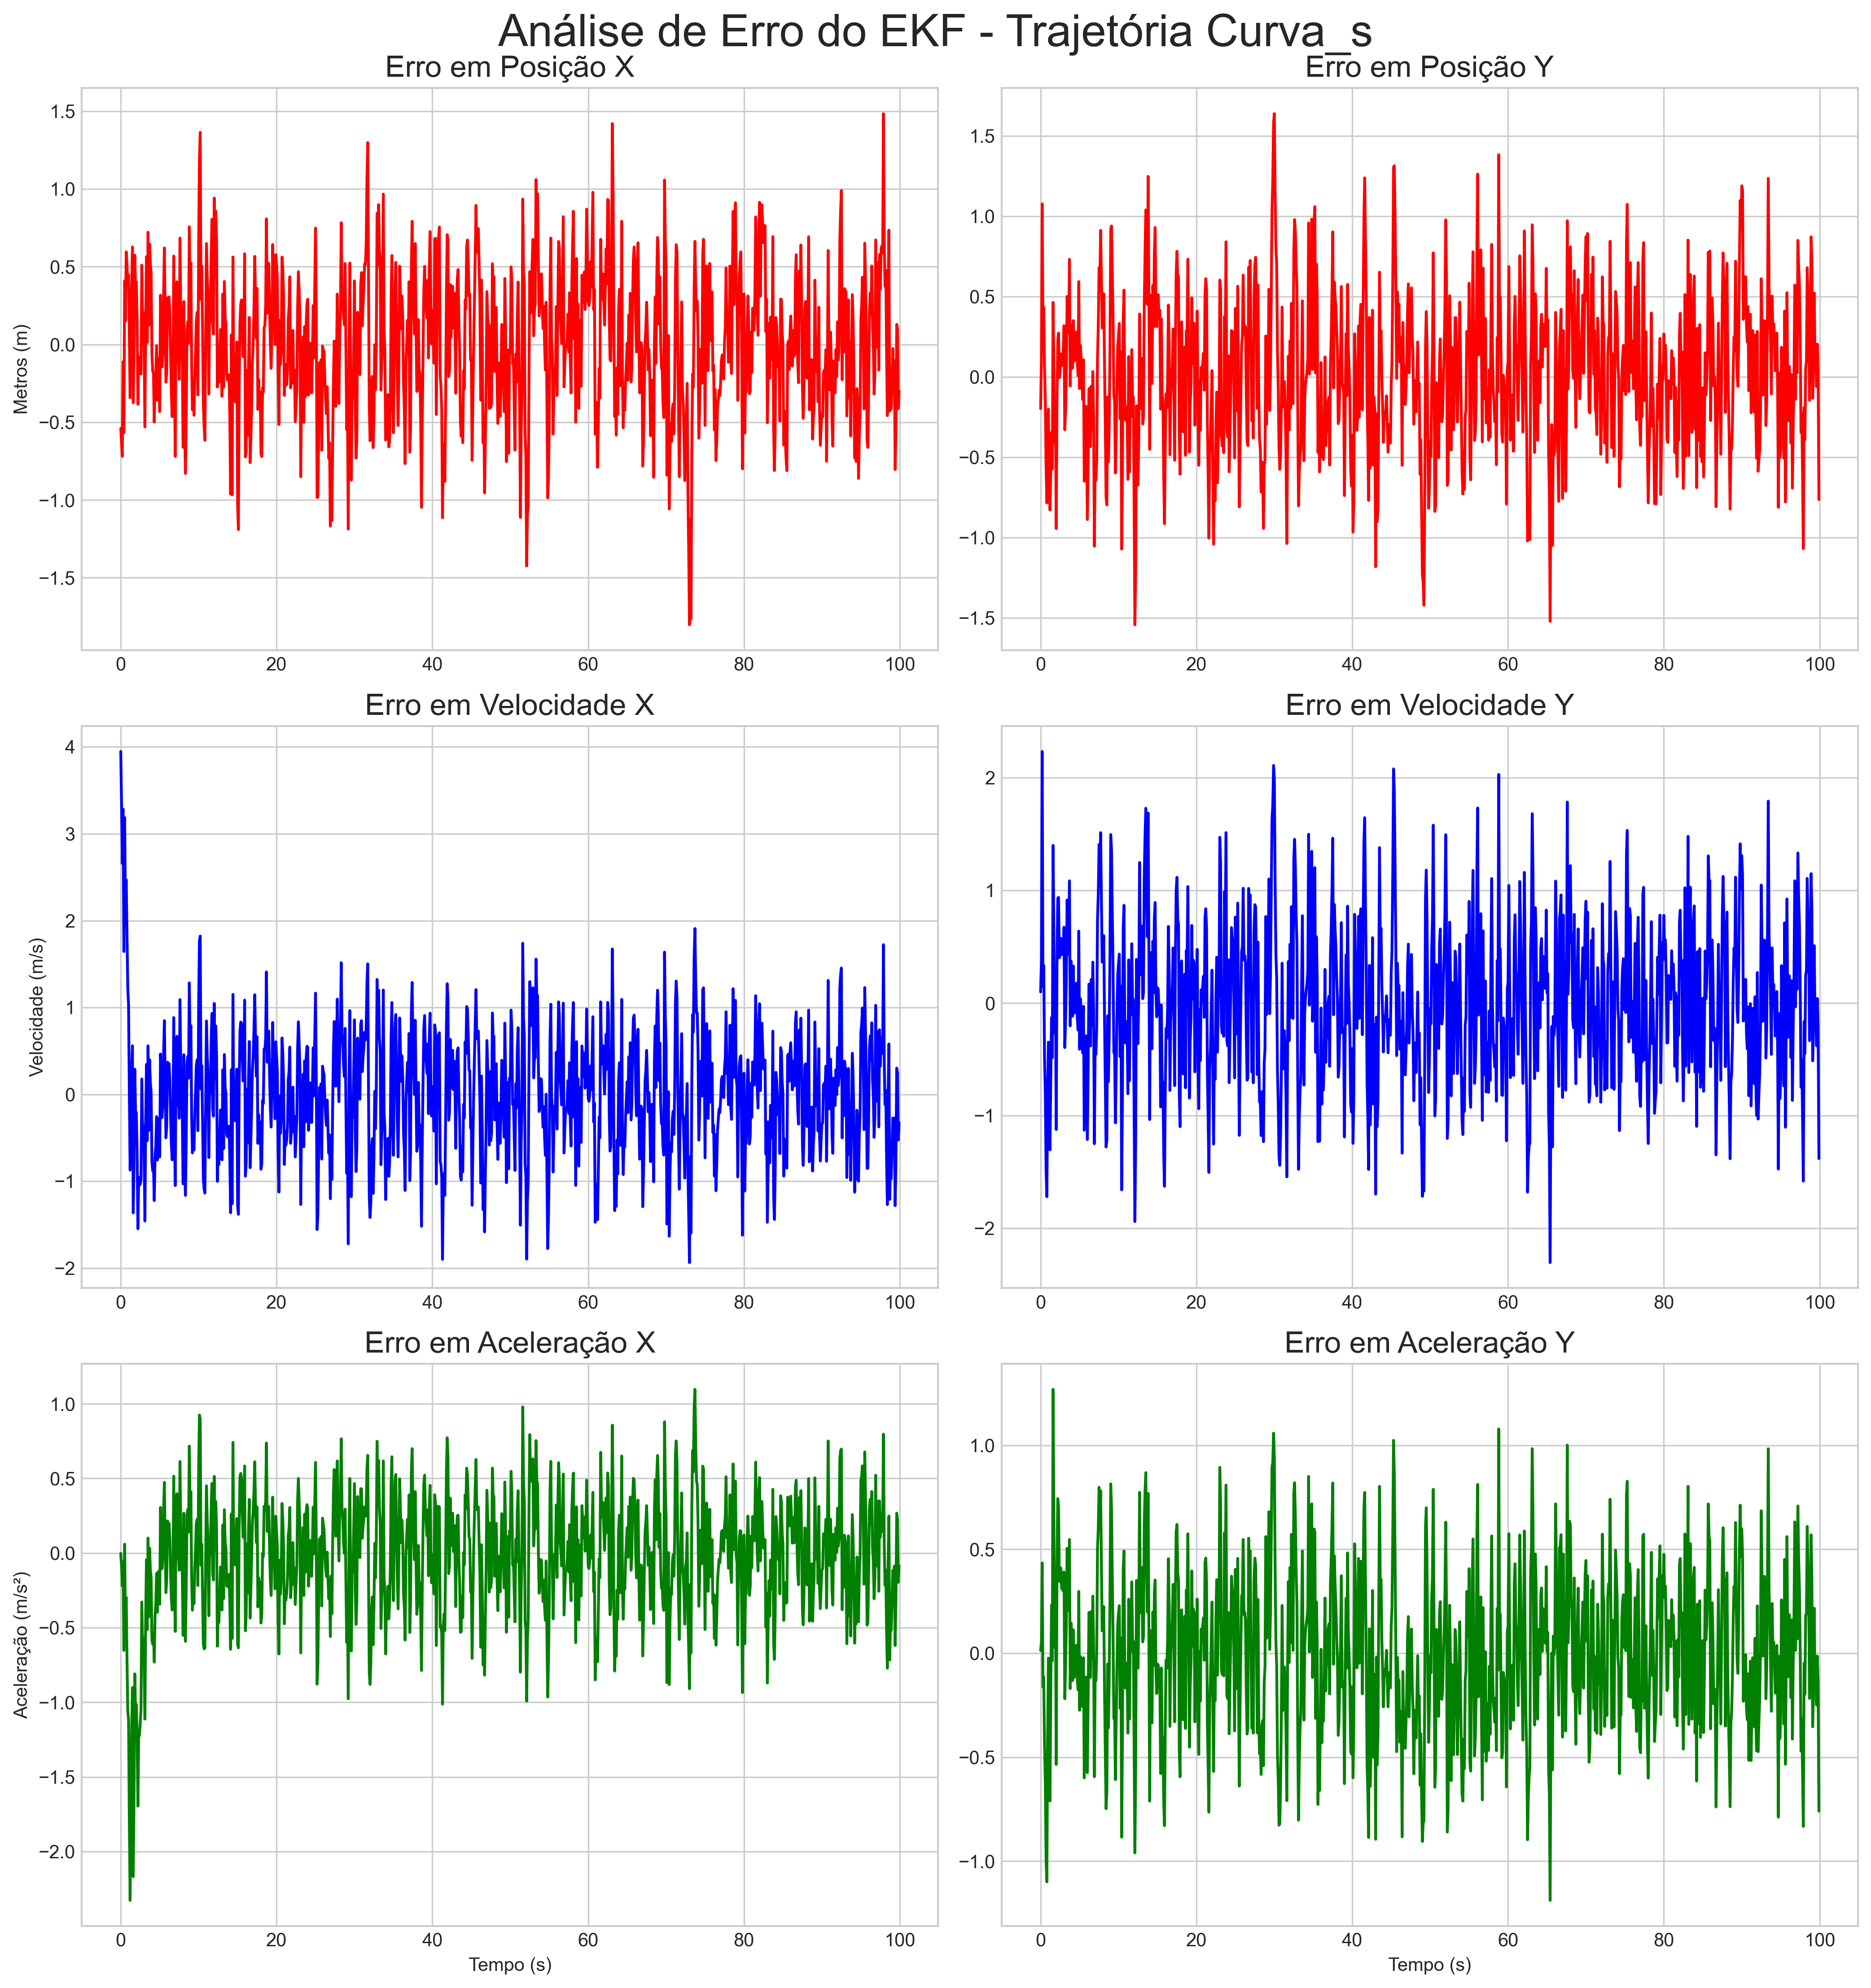
\includegraphics[width=0.85\linewidth]{Figuras/resultados/trajetoria_pva_curva_s/erros_estados_pva_curva_s.png}
        \label{fig:ErrosCurvaS}
        \vspace{2pt} % Pequeno ajuste de espaço
        \centerline{\footnotesize \textbf{Fonte:} Elaborado pelo autor (2026).}
\end{figure} 

Para as trajetórias analisadas, a simulação inicial com o EKF resultou nos dados consolidados apresentados na Tabela \ref{tab:resultados_estatisticos2}.

\begin{table}[t] % IEEE prefere [t] (top) ou [b] (bottom)
\centering
\footnotesize
\caption{Análise Estatística dos Erros de Estimação}
\label{tab:resultados_estatisticos2}
\setlength{\tabcolsep}{4pt} % Ajusta o espaçamento horizontal
\begin{tabular}{llcccc}
\toprule
\textbf{Traj.} & \textbf{Var.} & Bias X (\textbf{$\mu_x$}) & Bias Y (\textbf{$\mu_Y$}) & \textbf{RMS} & \textbf{DP ($\sigma$)} \\ 
\midrule
\multirow{3}{*}{Quadrada} & $P$ (m) & -0,021 & -0,032 & 0,717 & 0,716 \\
 & $V$ (m/s) & 0,006 & 0,037 & 2,328 & 2,328 \\
 & $A$ (m/s$^2$) & 0,012 & -0,373 & 1,692 & 1,650 \\ 
\midrule
\multirow{3}{*}{Circular} & $P$ (m) & -0,021 & -0,032 & 0,717 & 0,716 \\
 & $V$ (m/s) & 0,006 & 0,037 & 2,328 & 2,328 \\
 & $A$ (m/s$^2$) & 0,012 & -0,373 & 1,692 & 1,650 \\ 
\midrule
\multirow{3}{*}{Curva S} & $P$ (m) & -0,001 & 0,018 & 0,655 & 0,655 \\
 & $V$ (m/s) & 0,006 & 0,002 & 1,002 & 1,002 \\
 & $A$ (m/s$^2$) & -0,037 & 0,001 & 0,556 & 0,555 \\ 
\bottomrule
\multicolumn{6}{l}{\textit{Nota:} $P$: Posição; $V$: Velocidade; $A$: Aceleração.}
\end{tabular}
        \vspace{2pt} % Pequeno ajuste de espaço
        \centerline{\footnotesize \textbf{Fonte:} Elaborado pelo autor (2026).}
\end{table}

Analisando os resultados utilizando o algorítmo de identificação adaptativo,

\subsubsection{Análise Geral do desempenho da adaptação do Algorítmo}

A análise estrutural revelou que o sistema de localização não possui observabilidade suficiente para determinar univocamente as matrizes de ruído $\mathbf{Q}$ e $\mathbf{R}$. Conforme a Tabela \ref{tab:identificabilidade}, o posto da matriz de identificabilidade $\mathcal{I}$ manteve-se estritamente inferior ao número de incógnitas, mesmo ao simplificar o problema assumindo uma matriz $\mathbf{Q}$ diagonal.

\begin{table}[h]
\centering
\caption{Resumo da Identificabilidade do Sistema}
\label{tab:identificabilidade}
\begin{tabular}{lccc}
\hline
\textbf{Configuração de Q} & \textbf{Incógnitas} & \textbf{Posto de $\mathcal{I}$} & \textbf{Status} \\ \hline
Simétrica (Completa)       & 31                  & 21               & Não Identificável \\
Diagonal (Simplificada)    & 16                  & 15               & Não Identificável \\ \hline
\end{tabular}
        \vspace{2pt}
        \centerline{\footnotesize \textbf{Fonte:} Elaborado pelo autor (2026).}
\end{table}

Como consequência dessa limitação algébrica, o algoritmo adaptativo não conseguiu convergir para valores corretos em nenhuma das três trajetórias analisadas (quadrada, circular e curva em S). O processo de otimização divergiu, gerando matrizes de erro com magnitudes impróprias para o rastreamento e instabilidade numérica. Essa falha generalizada na convergência é, muito provavelmente, causada por uma combinação de fatores: não apenas as limitações da própria implementação computacional, mas também a imprecisão gerada pela aproximação do valor médio (a utilização da Jacobiana média $\mathbf{F}_{jac} \approx \mathbf{F}$) para contornar a não-linearidade geométrica do problema.
% -------------------------------
% SEÇÃO 6: CONCLUSÃO
% -------------------------------
\section{Conclusão}

\subsection{Síntese}

Os experimentos realizados com trajetórias quadrada, circular e curvilínea confirmaram que o Filtro de Kalman Estendido (EKF) é capaz de rastrear alvos com consistência estatística, validada pelo teste NIS e pela análise dos resíduos. No entanto, a estratégia de adaptação do algoritmo de identificação de covariâncias – que emprega Jacobianos médios ao longo da trajetória – não conduziu à convergência para as matrizes verdadeiras $\mathbf{Q}$ e $\mathbf{R}$.

A causa central dessa falha reside no fato de que a dinâmica média (representada pelos Jacobianos médios $\hat{\mathbf{F}}$ e $\hat{\mathbf{H}}$) não captura a variabilidade temporal inerente a trajetórias não lineares. Como consequência:

\begin{itemize}
    \item A matriz de identificabilidade do sistema é mal condicionada, prejudicando a separação dos efeitos do ruído de processo e de medição;
    \item A função objetivo minimizada ($J(\mathbf{W})$) deixa de representar a covariância real da inovação, desviando o otimizador do mínimo global;
    \item As estimativas finais de $\mathbf{Q}$ e $\mathbf{R}$ afastam-se significativamente dos valores de referência, acumulando erros que comprometem a acurácia do filtro.
\end{itemize}

Portanto, a abordagem de linearização por ponto de operação médio, embora conceitualmente simples, mostra-se inadequada para o caso não linear sem garantias de convergência, conforme já antecipado pelos autores do método original \cite{zhang2020}.

Não obstante o insucesso na convergência do algoritmo, a implementação computacional desenvolvida – incluindo a estrutura modular para simulação de trajetórias, o EKF genérico e o arcabouço do método adaptativo – permanece como um recurso útil para a comunidade. O código, organizado de forma clara e documentada, pode ser reutilizado, modificado e estendido por outros pesquisadores, facilitando a investigação de novas estratégias de identificação de covariâncias ou a adaptação do algoritmo para classes mais amplas de sistemas não lineares.

\subsection{Trabalhos Futuros}

Para superar as limitações observadas, propõe-se investigar extensões do algoritmo que incorporem a variação temporal dos Jacobianos, possivelmente por meio de técnicas de \textit{clustering} da trajetória ou de otimização conjunta sobre múltiplos regimes lineares. Adicionalmente, recomenda-se a implementação de aceleradores em GPU para viabilizar a execução em tempo real, bem como o aprofundamento teórico sobre a identificabilidade de sistemas não lineares variantes no tempo. Tais avanços são essenciais para a aplicação prática em robótica móvel e navegação autônoma, onde a adaptação dinâmica ao ruído ambiental é um requisito crítico de segurança e precisão.
% -------------------------------
% REFERÊNCIAS BIBLIOGRÁFICAS
% -------------------------------
\begin{thebibliography}{1}

\bibitem{kalman60}
R.~E. Kalman, ``A New Approach to Linear Filtering and Prediction Problems,'' \emph{Journal of Basic Engineering}, vol. 82, no. 1, pp. 35--45, 1960.

\bibitem{falek2020}
P.~Fałek and P.~Kaniewski, ``Computer application for testing Kalman filter,'' \emph{Journal of Automation, Mobile Robotics \& Intelligent Systems}, vol. 14, no. 2, pp. 3--10, 2020.

\bibitem{zhang2020}
L.~Zhang, D.~Sidoti, A.~Bienkowski, K.~R. Pattipati, Y.~Bar-Shalom, and D.~L. Kleinman, ``On the Identification of Noise Covariances and Adaptive Kalman Filtering: A New Look at a 50-Year-Old Problem,'' \emph{IEEE Access}, vol. 8, pp. 59362--59388, 2020. DOI: 10.1109/ACCESS.2020.2982407.

\bibitem{thrun05}
S.~Thrun, W.~Burgard, and D.~Fox, \emph{Probabilistic Robotics}. Cambridge, MA: MIT Press, 2005.
\bibitem{Neethling1974}
C. Neethling and J. L. Willems, ``The use of the innovations sequence to determine the state covariance matrix of a linear time-invariant system,'' \textit{Automatica}, vol. 10, no. 3, pp. 337--341, 1974.

\bibitem{Odelson2006}
B. J. Odelson, M. R. Rajamani, and J. B. Rawlings, ``A new pose for adaptive Kalman filtering: The monitoring and estimation of control performance,'' \textit{Control Engineering Practice}, vol. 14, no. 3, pp. 303--314, 2006.

\bibitem{Mehra1970}
R. K. Mehra, ``On the identification of variance and adaptive Kalman filtering,'' \textit{IEEE Transactions on Automatic Control}, vol. 15, no. 2, pp. 175--184, Apr. 1970.

\bibitem{chen2023kalman}
Z.~Chen, H.~Biggie, N.~Ahmed, S.~Julier, and C.~Heckman, ``Kalman Filter Auto-tuning through Enforcing Chi-Squared Normalized Error Distributions with Bayesian Optimization,'' \emph{arXiv preprint arXiv:2306.07225}, 2023.

\bibitem{BarShalom2001}
Y. Bar-Shalom, X. R. Li, e T. Kirubarajan, \textit{Estimation with Applications to Tracking and Navigation}. New York, NY, USA: John Wiley \& Sons, 2001.

\bibitem{carew1973}
B.~Carew and P.~R.~Bélanger, ``Identification of optimum filter steady-state gain for systems with unknown noise covariances,'' \emph{IEEE Transactions on Automatic Control}, vol. 18, no. 6, pp. 582--592, Dec. 1973.

\bibitem{chen2018weak}
Z.~Chen, C.~Heckman, and S.~Julier, ``Weak in the NEES?: Auto-tuning Kalman Filters with Bayesian Optimization,'' in \emph{2018 21st International Conference on Information Fusion (FUSION)}, 2018.

\end{thebibliography}

% -------------------------------
% BIOGRAFIA DO AUTOR
% -------------------------------
\begin{IEEEbiography}[{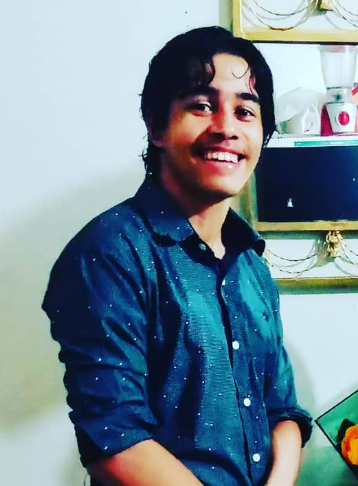
\includegraphics[width=1in,height=1.25in,clip,keepaspectratio]{Figuras/Basicos/autor.png}}]{Saulo José Almeida Silva}
Técnico em Eletrotécnica pelo Instituto Federal de Alagoas (IFAL, 2021). Bacharel em Engenharia Elétrica com ênfase em Eletrotécnica pelo IFAL (2026). Pós-graduação \emph{lato sensu} em Automação Industrial pela Eduno. Atualmente é mestrando em Engenharia Elétrica na Universidade Federal de Campina Grande (UFCG), atuando na área de Robótica, com foco em coordenação de sistemas robóticos heterogêneos.
\end{IEEEbiography}


% -------------------------------
% APÊNDICES
% -------------------------------
\newpage
\begin{appendices}
    


\section{Modelagem e Discretização do Sistema}
\label{app:discretizacao}

A dinâmica de sistemas robóticos móveis é frequentemente descrita por modelos representados em espaço de estados no tempo contínuo. Considere o sistema linear e invariante no tempo (LTI) definido por:
\begin{align}
\dot{\mathbf{x}}(t) &= \mathbf{A} \mathbf{x}(t) + \mathbf{B} \mathbf{u}(t) + \mathbf{\Gamma} \mathbf{w}(t) \label{eq:ss_cont} \\
\mathbf{z}(t) &= \mathbf{C} \mathbf{x}(t) + \mathbf{v}(t)
\end{align}
onde $\mathbf{x}(t) \in \mathbb{R}^n$ é o vetor de estados, $\mathbf{u}(t) \in \mathbb{R}^m$ é o vetor de controle e $\mathbf{z}(t) \in \mathbb{R}^p$ é o vetor de medições. Os ruídos de processo $\mathbf{w}(t)$ e de medição $\mathbf{v}(t)$ são assumidos como processos de Gauss-Markov brancos, independentes, com densidades espectrais de potência $\mathbf{Q}_c$ e $\mathbf{R}_c$, respectivamente, e $\mathbf{\Gamma}$ representa a matriz de acoplamento do ruído do processo.

Utilizando a abordagem descrita em \cite{chen2023kalman}, para a implementação em sistemas digitais com período de amostragem $\Delta t$, o modelo contínuo é transformado em seu equivalente discreto. Sob a premissa de um Segurador de Ordem Zero (ZOH) aplicado às entradas de controle, o sistema é representado nos instantes $t_k = k \Delta t$ por:
\begin{align}
\mathbf{x}_k &= \mathbf{F} \mathbf{x}_{k-1} + \mathbf{G} \mathbf{u}_{k-1} + \mathbf{w}_{k-1} \label{eq:ss_disc} \\
\mathbf{z}_k &= \mathbf{H} \mathbf{x}_k + \mathbf{v}_k
\end{align}
onde as matrizes do sistema discreto são $\mathbf{F}$ (transição de estados), $\mathbf{G}$ (entrada) e $\mathbf{H}$ (observação). As sequências de ruído discretas possuem propriedades estatísticas $\mathbf{w}_{k-1} \sim \mathcal{N}(\mathbf{0}, \mathbf{Q}_k)$ e $\mathbf{v}_k \sim \mathcal{N}(\mathbf{0}, \mathbf{R}_k)$. Cabe ressaltar que o efeito de $\mathbf{\Gamma}$ já se encontra embutido na covariância discreta $\mathbf{Q}_k$.

\section{Matrizes de Transição e Controle}

A matriz de transição de estados $\mathbf{F}$ e a matriz de entrada discreta $\mathbf{G}$ são obtidas através da solução da equação diferencial de estados sobre o intervalo de amostragem $\Delta t$:
\begin{equation}
\mathbf{F} = e^{\mathbf{A} \Delta t}, \quad \mathbf{G} = \left( \int_{0}^{\Delta t} e^{\mathbf{A} \tau} \, d\tau \right) \mathbf{B}
\end{equation}

Computacionalmente, uma abordagem eficiente para o cálculo simultâneo dessas matrizes consiste na exponencial de uma matriz em bloco aumentada, conforme o método de Van Loan:
\begin{equation}
\exp\left( \begin{bmatrix} \mathbf{A} & \mathbf{B} \\ \mathbf{0} & \mathbf{0} \end{bmatrix} \Delta t \right) = \begin{bmatrix} \mathbf{F} & \mathbf{G} \\ \mathbf{0} & \mathbf{I} \end{bmatrix}
\end{equation}

\section{Covariâncias dos Ruídos Discretos}

A matriz de covariância do ruído de processo discreto $\mathbf{Q}_k$ é derivada da integração da dinâmica do ruído contínuo, ponderada pela matriz de transição e considerando explicitamente a matriz de acoplamento de ruído $\mathbf{\Gamma}$:
\begin{equation}
\mathbf{Q}_k = \int_{0}^{\Delta t} e^{\mathbf{A} \tau} \mathbf{\Gamma} \mathbf{Q}_c \mathbf{\Gamma}^T e^{\mathbf{A}^T \tau} \, d\tau
\end{equation}

\section{Repositório do Código Fonte}
\label{app:code}
O código completo da implementação está disponível publicamente em: \\
\url{https://encurtador.com.br/zfrI}.

\section{Matrizes Positivas Semidefinidas}
\label{app:PSD}

Uma matriz quadrada e simétrica $\mathbf{A} \in \mathbb{R}^{n \times n}$ é classificada como positiva semidefinida (condição denotada por $\mathbf{A} \succeq 0$) se a sua forma quadrática for não negativa para qualquer vetor real não nulo $\mathbf{x} \in \mathbb{R}^n$:

\begin{equation}
    \label{eq:psd_def}
    \mathbf{x}^\top \mathbf{A} \mathbf{x} \ge 0
\end{equation}

De forma equivalente, pelo teorema espectral, $\mathbf{A}$ é positiva semidefinida se, e somente se, todos os seus autovalores forem maiores ou iguais a zero. 

\section{Norma de Frobenius}
\label{app:frobenius}

A norma de Frobenius é uma métrica utilizada para quantificar a magnitude de uma matriz. Para uma matriz real $\mathbf{A} \in \mathbb{R}^{m \times n}$, a norma de Frobenius, denotada por $\|\mathbf{A}\|_F$, é definida como a raiz quadrada da soma dos quadrados de todos os seus elementos:

\begin{equation}
    \label{eq:frob_def1}
    \|\mathbf{A}\|_F = \sqrt{\sum_{i=1}^{m} \sum_{j=1}^{n} a_{ij}^2}
\end{equation}

Algebricamente, esta norma também pode ser calculada de forma equivalente e computacionalmente eficiente utilizando o operador traço ($\operatorname{tr}$):

\begin{equation}
    \label{eq:frob_def2}
    \|\mathbf{A}\|_F = \sqrt{\operatorname{tr}(\mathbf{A}^\top \mathbf{A})}
\end{equation}

No contexto do algoritmo proposto, a norma de Frobenius é aplicada nos critérios de convergência para avaliar a distância entre as estimativas de uma mesma matriz (como $\mathbf{W}$, $\mathbf{Q}$ e $\mathbf{R}$) em iterações sucessivas, permitindo mensurar a estabilização do processo iterativo.

\section{Aproximação Numérica da Matriz Jacobiana por Diferenças Finitas}
\label{app:jacobiana_num}

O método de diferenças finitas é uma técnica numérica utilizada para aproximar derivadas de funções onde a obtenção analítica é inviável ou computacionalmente custosa. A abordagem mais precisa é a de \textit{diferenças centrais}, que aproxima a derivada de uma função univariada $f(x)$ através de incrementos simétricos $\delta$:
\begin{equation}
    f'(x) \approx \frac{f(x+\delta) - f(x-\delta)}{2\delta}
\end{equation}

Para funções multivariadas e vetoriais $\mathbf{h}(\mathbf{x})$, que mapeiam um vetor de entrada $\mathbf{x} \in \mathbb{R}^n$ para um vetor de saída em $\mathbb{R}^m$, a generalização do gradiente resulta na Matriz Jacobiana $\mathbf{H} \in \mathbb{R}^{m \times n}$.

Utilizando o método de diferenças centrais, a matriz Jacobiana pode ser construída computacionalmente calculando-se uma coluna de cada vez. Seja $\mathbf{e}_j$ o vetor base canônico de dimensão $n$ (contendo o valor $1$ na $j$-ésima posição e $0$ nas demais), a $j$-ésima coluna da matriz Jacobiana representa a derivada parcial da função em relação à variável $x_j$, aproximada pela Equação \eqref{eq:jacobiana_coluna}.

\begin{equation}
    \label{eq:jacobiana_coluna}
    \mathbf{H}_{:, j} = \frac{\partial \mathbf{h}}{\partial x_j} \approx \frac{\mathbf{h}(\mathbf{x} + \delta \mathbf{e}_j) - \mathbf{h}(\mathbf{x} - \delta \mathbf{e}_j)}{2\delta}
\end{equation}

A matriz completa é montada de forma sistemática aplicando a Equação \eqref{eq:jacobiana_coluna} iterativamente para cada variável $j = 1, 2, \dots, n$, concatenando os vetores colunas resultantes lado a lado, conforme a Equação \eqref{eq:jacobiana_completa}.

\begin{equation}
    \label{eq:jacobiana_completa}
    \mathbf{H} \approx \begin{bmatrix}
        | & | & & | \\
        \mathbf{H}_{:, 1} & \mathbf{H}_{:, 2} & \dots & \mathbf{H}_{:, n} \\
        | & | & & |
    \end{bmatrix}
\end{equation}

\section{Consistência Estatística via Normalized Innovation Squared (NIS)}
\label{app:NIS}

O teste NIS (\textit{Normalized Innovation Squared}) é uma métrica estatística utilizada para avaliar a consistência de um Filtro de Kalman. Ele verifica se as suposições teóricas sobre as covariâncias de ruído do processo ($\mathbf{Q}$) e de medição ($\mathbf{R}$) são condizentes com os resíduos observados na prática.

A inovação, denotada por $\boldsymbol{\nu}_k$, representa o erro residual entre a medição real $\mathbf{z}_k$ e a predição da medição baseada no modelo de estados:
\begin{equation}
    \boldsymbol{\nu}_k = \mathbf{z}_k - \mathbf{H}\hat{\mathbf{x}}_{k|k-1}
\end{equation}

A covariância teórica associada a essa inovação é definida por $\mathbf{S}_k$. O escalar NIS é calculado como a forma quadrática da inovação ponderada pelo inverso de sua covariância:
\begin{equation}
    \label{eq:calculo_nis}
    \epsilon_k = \boldsymbol{\nu}_k^\top \mathbf{S}_k^{-1} \boldsymbol{\nu}_k
\end{equation}

\label{app:ChiChen}

Sob a hipótese de que o filtro está corretamente sintonizado e os ruídos são gaussianos, a variável $\epsilon_k$ segue uma distribuição Qui-quadrado ($\chi^2$) com $n_z$ graus de liberdade, onde $n_z$ é a dimensão do vetor de medição. 

Para uma análise de desempenho global, utiliza-se a média do NIS ao longo de um horizonte de $N$ amostras. O valor esperado da média deve aproximar-se do número de medições:
\begin{equation}
    \label{eq:media_nis}
    E[\bar{\epsilon}] = E \left[ \frac{1}{N} \sum_{k=1}^{N} \epsilon_k \right] = n_z
\end{equation}

A interpretação do NIS permite diagnosticar o estado de sintonia do filtro:
\begin{itemize}
    \item \textbf{Consistente:} Se $\bar{\epsilon} \approx n_z$, o filtro é considerado estatisticamente consistente.
    \item \textbf{Otimista:} Se $\bar{\epsilon} > n_z$, as inovações são maiores do que a incerteza prevista por $\mathbf{S}_k$, indicando que o filtro subestima os erros reais.
    \item \textbf{Conservador:} Se $\bar{\epsilon} < n_z$, as inovações são menores do que o previsto, sugerindo que as matrizes de ruído fornecidas são excessivamente altas.
\end{itemize}

Para maiores detalhes sobre a análise estatística de filtros lineares e testes de hipóteses sobre a inovação, recomenda-se a consulta à obra de referência de \cite{BarShalom2001} e \cite{chen2023kalman}

% Referência para adicionar ao seu BibTeX:
% BAR-SHALOM, Y.; LI, X. R.; KIRUBARAN, T. Estimation with Applications to Tracking and Navigation. New York: John Wiley & Sons, 2001.

\end{appendices}

\end{document}